\documentclass[]{book}
\usepackage{lmodern}
\usepackage{amssymb,amsmath}
\usepackage{ifxetex,ifluatex}
\usepackage{fixltx2e} % provides \textsubscript
\ifnum 0\ifxetex 1\fi\ifluatex 1\fi=0 % if pdftex
  \usepackage[T1]{fontenc}
  \usepackage[utf8]{inputenc}
\else % if luatex or xelatex
  \ifxetex
    \usepackage{mathspec}
  \else
    \usepackage{fontspec}
  \fi
  \defaultfontfeatures{Ligatures=TeX,Scale=MatchLowercase}
    \setmonofont[Mapping=tex-ansi]{Source Code Pro}
\fi
% use upquote if available, for straight quotes in verbatim environments
\IfFileExists{upquote.sty}{\usepackage{upquote}}{}
% use microtype if available
\IfFileExists{microtype.sty}{%
\usepackage[]{microtype}
\UseMicrotypeSet[protrusion]{basicmath} % disable protrusion for tt fonts
}{}
\PassOptionsToPackage{hyphens}{url} % url is loaded by hyperref
\usepackage[unicode=true]{hyperref}
\hypersetup{
            pdftitle={Technical Foundations of Informatics},
            pdfauthor={Michael Freeman and Joel Ross},
            pdfborder={0 0 0},
            breaklinks=true}
\urlstyle{same}  % don't use monospace font for urls
\usepackage{natbib}
\bibliographystyle{plainnat}
\usepackage{color}
\usepackage{fancyvrb}
\newcommand{\VerbBar}{|}
\newcommand{\VERB}{\Verb[commandchars=\\\{\}]}
\DefineVerbatimEnvironment{Highlighting}{Verbatim}{commandchars=\\\{\}}
% Add ',fontsize=\small' for more characters per line
\usepackage{framed}
\definecolor{shadecolor}{RGB}{248,248,248}
\newenvironment{Shaded}{\begin{snugshade}}{\end{snugshade}}
\newcommand{\KeywordTok}[1]{\textcolor[rgb]{0.13,0.29,0.53}{\textbf{#1}}}
\newcommand{\DataTypeTok}[1]{\textcolor[rgb]{0.13,0.29,0.53}{#1}}
\newcommand{\DecValTok}[1]{\textcolor[rgb]{0.00,0.00,0.81}{#1}}
\newcommand{\BaseNTok}[1]{\textcolor[rgb]{0.00,0.00,0.81}{#1}}
\newcommand{\FloatTok}[1]{\textcolor[rgb]{0.00,0.00,0.81}{#1}}
\newcommand{\ConstantTok}[1]{\textcolor[rgb]{0.00,0.00,0.00}{#1}}
\newcommand{\CharTok}[1]{\textcolor[rgb]{0.31,0.60,0.02}{#1}}
\newcommand{\SpecialCharTok}[1]{\textcolor[rgb]{0.00,0.00,0.00}{#1}}
\newcommand{\StringTok}[1]{\textcolor[rgb]{0.31,0.60,0.02}{#1}}
\newcommand{\VerbatimStringTok}[1]{\textcolor[rgb]{0.31,0.60,0.02}{#1}}
\newcommand{\SpecialStringTok}[1]{\textcolor[rgb]{0.31,0.60,0.02}{#1}}
\newcommand{\ImportTok}[1]{#1}
\newcommand{\CommentTok}[1]{\textcolor[rgb]{0.56,0.35,0.01}{\textit{#1}}}
\newcommand{\DocumentationTok}[1]{\textcolor[rgb]{0.56,0.35,0.01}{\textbf{\textit{#1}}}}
\newcommand{\AnnotationTok}[1]{\textcolor[rgb]{0.56,0.35,0.01}{\textbf{\textit{#1}}}}
\newcommand{\CommentVarTok}[1]{\textcolor[rgb]{0.56,0.35,0.01}{\textbf{\textit{#1}}}}
\newcommand{\OtherTok}[1]{\textcolor[rgb]{0.56,0.35,0.01}{#1}}
\newcommand{\FunctionTok}[1]{\textcolor[rgb]{0.00,0.00,0.00}{#1}}
\newcommand{\VariableTok}[1]{\textcolor[rgb]{0.00,0.00,0.00}{#1}}
\newcommand{\ControlFlowTok}[1]{\textcolor[rgb]{0.13,0.29,0.53}{\textbf{#1}}}
\newcommand{\OperatorTok}[1]{\textcolor[rgb]{0.81,0.36,0.00}{\textbf{#1}}}
\newcommand{\BuiltInTok}[1]{#1}
\newcommand{\ExtensionTok}[1]{#1}
\newcommand{\PreprocessorTok}[1]{\textcolor[rgb]{0.56,0.35,0.01}{\textit{#1}}}
\newcommand{\AttributeTok}[1]{\textcolor[rgb]{0.77,0.63,0.00}{#1}}
\newcommand{\RegionMarkerTok}[1]{#1}
\newcommand{\InformationTok}[1]{\textcolor[rgb]{0.56,0.35,0.01}{\textbf{\textit{#1}}}}
\newcommand{\WarningTok}[1]{\textcolor[rgb]{0.56,0.35,0.01}{\textbf{\textit{#1}}}}
\newcommand{\AlertTok}[1]{\textcolor[rgb]{0.94,0.16,0.16}{#1}}
\newcommand{\ErrorTok}[1]{\textcolor[rgb]{0.64,0.00,0.00}{\textbf{#1}}}
\newcommand{\NormalTok}[1]{#1}
\usepackage{longtable,booktabs}
% Fix footnotes in tables (requires footnote package)
\IfFileExists{footnote.sty}{\usepackage{footnote}\makesavenoteenv{long table}}{}
\usepackage{graphicx,grffile}
\makeatletter
\def\maxwidth{\ifdim\Gin@nat@width>\linewidth\linewidth\else\Gin@nat@width\fi}
\def\maxheight{\ifdim\Gin@nat@height>\textheight\textheight\else\Gin@nat@height\fi}
\makeatother
% Scale images if necessary, so that they will not overflow the page
% margins by default, and it is still possible to overwrite the defaults
% using explicit options in \includegraphics[width, height, ...]{}
\setkeys{Gin}{width=\maxwidth,height=\maxheight,keepaspectratio}
\usepackage[normalem]{ulem}
% avoid problems with \sout in headers with hyperref:
\pdfstringdefDisableCommands{\renewcommand{\sout}{}}
\IfFileExists{parskip.sty}{%
\usepackage{parskip}
}{% else
\setlength{\parindent}{0pt}
\setlength{\parskip}{6pt plus 2pt minus 1pt}
}
\setlength{\emergencystretch}{3em}  % prevent overfull lines
\providecommand{\tightlist}{%
  \setlength{\itemsep}{0pt}\setlength{\parskip}{0pt}}
\setcounter{secnumdepth}{5}
% Redefines (sub)paragraphs to behave more like sections
\ifx\paragraph\undefined\else
\let\oldparagraph\paragraph
\renewcommand{\paragraph}[1]{\oldparagraph{#1}\mbox{}}
\fi
\ifx\subparagraph\undefined\else
\let\oldsubparagraph\subparagraph
\renewcommand{\subparagraph}[1]{\oldsubparagraph{#1}\mbox{}}
\fi

% set default figure placement to htbp
\makeatletter
\def\fps@figure{htbp}
\makeatother

\usepackage{booktabs}
\usepackage{amsthm}
\usepackage{float}
\makeatletter
\def\thm@space@setup{%
  \thm@preskip=8pt plus 2pt minus 4pt
  \thm@postskip=\thm@preskip
}
\makeatother

\title{Technical Foundations of Informatics}
\author{\href{http://mfviz.com/\#/}{Michael Freeman} and
\href{http://faculty.washington.edu/joelross/}{Joel Ross}}
\date{August 23, 2017}

\usepackage{amsthm}
\newtheorem{theorem}{Theorem}[chapter]
\newtheorem{lemma}{Lemma}[chapter]
\theoremstyle{definition}
\newtheorem{definition}{Definition}[chapter]
\newtheorem{corollary}{Corollary}[chapter]
\newtheorem{proposition}{Proposition}[chapter]
\theoremstyle{definition}
\newtheorem{example}{Example}[chapter]
\theoremstyle{remark}
\newtheorem*{remark}{Remark}
\begin{document}
\maketitle

{
\setcounter{tocdepth}{2}
\tableofcontents
}
\chapter*{About this Book}\label{about-this-book}


This book covers the foundation skills necessary to start
\textbf{\emph{writing computer programs to work with data}} using modern
and reproducable techniques. It requires no technical background. These
materials were developed for the \textbf{INFO 201: Technical Foundations
of Informatics} course taught at the
\href{https://ischool.uw.edu/}{University of Washington Information
School}; however they have been structured to be an online resource for
anyone hoping to learn to work with information using programmatic
approaches.

This book is currently in \textbf{beta} status. Visit us on
\href{https://github.com/info201/book}{GitHub} to contribute
improvements.

\includegraphics{img/index/by-nc-sa.png} This book is licensed under a
\href{http://creativecommons.org/licenses/by-nc-sa/4.0/}{Creative
Commons Attribution-NonCommercial-ShareAlike 4.0 International License}.

\hypertarget{setup-machine}{\chapter{Setting up your
Machine}\label{setup-machine}}

We'll be using a variety of different software programs to write,
manage, and execute the code that we write. Unfortunately, one of the
most frustrating and confusing barriers to working with code is simply
getting your machine properly set up. This chapter aims to provide
sufficient information for setting up your machine, and troubleshooting
the process.

Note that iSchool lab machines should have all appropriate software
already installed and ready to use.

In short, you'll need to install the following programs: see below for
more information / options.

\begin{itemize}
\item
  \textbf{Git}: A set of tools for tracking changes to computer code
  (especially when collaborating with others). This program is already
  installed on Macs.

  \begin{itemize}
  \tightlist
  \item
    \textbf{GitHub}: A web service for hosting code online. You don't
    actually need to \emph{install} anything GitHub (it uses
    \texttt{git}), but you'll need to sign up for the service.
  \end{itemize}
\item
  \textbf{Bash}: A \emph{command-line interface} for controlling your
  computer. \texttt{git} is a command-line program so you'll need a
  command shell to use it. Macs already have a Bash program called
  \emph{Terminal}. On Windows, installing \texttt{git} will also install
  a Bash shell called \emph{Git Bash}, or you can try the (experimental)
  Linux subsystem for Windows 10.
\item
  \textbf{Atom}: A lightweight text editor that supports programming in
  lots of different languages.

  \begin{itemize}
  \tightlist
  \item
    You are welcome to use another text editor if you wish; some further
    suggestions are included.
  \end{itemize}
\item
  \textbf{R}: a programming language commonly used for working with
  data. This is the primary programming language used throught this
  book. ``Installing R'' actually means installing tools that will let
  your computer understand and run R code.
\item
  \textbf{RStudio}: An graphical editor for writing and running R code.
  This will soon become our primary development application.
\end{itemize}

The following sections have additional information about the purpose of
each component, how to install it, and alternative configurations.

\section{Git}\label{git}

\textbf{\texttt{git}} is a version control system that provides a set of
commands that allow you to manage changes to written code, particularly
when collaborating with other programmers (much more on this in
\protect\hyperlink{git-basics}{chapter 4}). To start, you'll need to
\href{https://git-scm.com/downloads}{download} and install the software.
If you are on a Mac, \texttt{git} should already be installed.

If you are using a Windows machine, this will also install a program
called Git Bash, which provides a text-based interface for executing
commands on your computer. For alternative/additional Windows
command-line tools, see below.

\subsection{GitHub}\label{github}

GitHub is a website that is used to store copies of computer code that
are being managed with \texttt{git} (think ``Imgur for code''). Students
in the INFO 201 course will use GitHub to turn in programming
assignments.

In order to use GitHub, you'll need to
\href{https://github.com/join}{create a free GitHub account}, if you
don't already have one. You should register a username that is
identifiable as you (e.g., based on your name or your UW NetID). This
will make it easier for others to determine out who contributed what
code, rather than needing to figure out who `LeetDesigner2099' is. This
can be the start of a professional account you may use for the rest of
your career!

\section{Command-line Tools (Bash)}\label{command-line-tools-bash}

The command-line provides a text-based interface for giving instructions
to your computer (much more on this in
\protect\hyperlink{command-line}{chapter 2}). With this book, you'll
largely use the command-line for navigating your computer's file
structure, and executing commands that allows you to keep track of
changes to the code you write (i.e., version control with \texttt{git}).

In order to use the command-line, you will need to use a \textbf{command
shell} (a.k.a. a \emph{command prompt}). This is a program that provides
the interface to type commands into. In particular, we'll be working
with the Bash shell, which provides a particular common set of commands
common to Mac and Linux machines.

\subsection{Command-line on a Mac}\label{command-line-on-a-mac}

On a Mac you'll want to use the built-in app called \emph{Terminal}. You
can open it by searching via Spotlight (hit Cmd (\texttt{⌘}) and
Spacebar together, type in ``terminal'', then select the app to open
it), or by finding it in the Applications/Utilities folder.

\subsection{Command-line on Windows}\label{command-line-on-windows}

On Windows, we recommend using
\href{https://git-scm.com/downloads}{\textbf{Git Bash}}, which you
should have installed along with \texttt{git} (above). Open this program
to open the command-shell. This works great, since you'll primarily be
using the command-line for performing version control.

\begin{itemize}
\tightlist
\item
  Note that Windows does come with its own command-prompt, called the
  \emph{DOS Prompt}, but it has a different set of commands and
  features. \emph{Powershell} is a more powerful version of the DOS
  prompt if you really want to get into the Windows Management
  Framework. But Bash is more common in open-source programming like
  we'll be doing, and so we will be focusing on that set of commands.
\end{itemize}

Alternatively, the 64-bit Windows 10 Anniversary update (August 2016)
\emph{does} include a beta version of an integrated Bash shell. You can
access this by
\href{https://msdn.microsoft.com/en-us/commandline/wsl/install_guide}{enabling
the subsystem for Linux} and then running \texttt{bash} in the command
prompt. This is currently (May 2017) ``beta'' technology, but will
suffice for our purposes if you can get it running.

\section{Text Editors}\label{text-editors}

In order to produce computer code, you need somewhere to write it (and
we don't want to write it in MS Word!). There are a variety of available
programs that provide an interface for editing code. A major advantage
of these programs is that they provide automatic formatting/coloring for
easier interpretation of the code, along with cool features like
auto-completion and integration with version control.

RStudio has a great built-in text editor, but you'll sometimes want to
use another text editor which is lighter weight (e.g., runs faster),
more robust, or supports a different programming language. There are
lots of different text editors out there, all of which have slightly
different appearances and features. You only need to download and use
one of the following programs (we recommend \textbf{Atom} as a default),
but feel free to try out different ones to find something you like (and
then evangelize about it to your friends!)

\subsection{Atom}\label{atom}

\href{https://atom.io/}{\textbf{Atom}} is a text editor built by the
folks at GitHub and has been gaining in popularity. As an open source
project, people are continually building (and making available)
interesting/useful extensions. Its built-in spell-check is a great
feature, especially for documents that require lots of written text. It
also has excellent support for Markdown, a markup language you'll be
using regularly in this course.

To Download Atom, visit their \href{https://atom.io/}{\textbf{webpage}}
and click the ``Download'' button to download the installer
\texttt{.exe} file, then double-click on that icon to install the
application.

Once you've installed Atom, you can open the program and create a new
text file. When you save a document that is a particular file-type
(i.e., \texttt{file-name.R}, or \texttt{file-name.md}), Atom (or any
other modern text-editor) will apply a language specific color scheme to
your text, making it easier to read.

The trick to using Atom more efficiently is to get comfortable with the
\href{http://flight-manual.atom.io/getting-started/sections/atom-basics/\#command-palette}{Command
Palette}. If you hit \texttt{Cmd+Shift+P}, Atom will open a small window
where you can search for whatever you want the editor to do. For
example, if you type in \texttt{markdown} you can get list of commands
related to Markdown files (including the ability to open up a preview).

For more information about using Atom, see
\href{http://flight-manual.atom.io/}{the manual}.

\subsection{Visual Studio Code}\label{visual-studio-code}

\href{https://code.visualstudio.com/}{\textbf{Visual Studio Code}} (or
VS Code; not to be confused with Visual Studio) is a free, open-source
editor developed by Microsoft---yes, really. While it focuses on web
programming and JavaScript, it readily supports lots of languages
including Markdown and R and provides a number of extensions for adding
even more features. It has a similar \emph{command palette} to Atom, but
isn't quite as nice for editing Markdown specifically. Although fairly
new, it is updated regularly and has become one of our main editors for
programming.

\subsection{Sublime Text}\label{sublime-text}

\href{https://www.sublimetext.com/3}{\textbf{Sublime Text}} is a very
popular text editor with excellent defaults and a variety of available
extensions (though you'll need to manage and install extensions to
achieve the functionality offered by other editors out of the box).
While the software can be used for free, every 20 or so saves it will
prompt you to purchase the full version.

\section{R Language}\label{r-language}

The primary programming language you will use throughout this book is
called \href{https://www.r-project.org/}{\textbf{R}}. It's a very
powerful statistical programming language that is built to work well
with large and diverse datasets. See the
\emph{\protect\hyperlink{r-intro}{Introduction to R}} chapter for a more
in-depth introduciton to the language.

In order to program with R, you will need to install the \textbf{\emph{R
Interpreter}} on your machine. This is a piece of software that is able
to ``read'' code written in R and use that code to control your
computer, thereby ``programming'' it.

The easiest way to install R is to download it from the Comprehensive R
Archive Network (CRAN) at \textbf{\url{https://cran.rstudio.com/}}.
Click on the appropriate link for your operating system in order to find
a link to the installer.

\begin{itemize}
\tightlist
\item
  On a Mac, you're looking for the \texttt{.pkg} file---get the latest
  version supported by your computer.
\item
  On Windows, following the link to the \texttt{base} subdirectory (or
  following the link to ``\emph{install R for the first time}''), then
  click the link to download the latest version of R for Windows. You
  will need to double-click on the \texttt{.exe} file to install the
  software.
\end{itemize}

\section{RStudio}\label{rstudio}

While you are able to execute R scripts without an interface, the
\textbf{RStudio} application provides a wonderful way to engage with the
R language. RStudio is described in more detail in
\emph{\protect\hyperlink{r-intro}{Introduction to R}}

To install the RStudio program, select the \textbf{installer} for your
operating system from the
\href{https://www.rstudio.com/products/rstudio/download/}{downloads
page}. Make sure to download the \textbf{\emph{free}} version:

\begin{figure}
\centering
\includegraphics{img/setup/rstudio-download.png}
\caption{File to choose for downloading RStudio. Image may not show the
latest version.}
\end{figure}

Once the download completes, double-click on the \texttt{.exe} or
\texttt{.dmg} file to run the installer. Simply follow the steps of the
installer, and you should be prepared to use RStudio.

\hypertarget{resources}{\section*{Resources}\label{resources}}


Links to the recommended software are collected here for easy access:

\begin{itemize}
\tightlist
\item
  \href{https://git-scm.com/downloads}{git (and Git Bash)}

  \begin{itemize}
  \tightlist
  \item
    \href{https://github.com/join}{GitHub} (sign up)
  \item
    optional:
    \href{https://msdn.microsoft.com/en-us/commandline/wsl/install_guide}{Bash
    on Windows}
  \end{itemize}
\item
  \href{https://atom.io/}{Atom}
\item
  \href{https://cran.rstudio.com/}{R}
\item
  \href{https://www.rstudio.com/products/rstudio/download3/}{RStudio}
\end{itemize}

\hypertarget{command-line}{\chapter{The Command
Line}\label{command-line}}

The \textbf{command-line} is an \emph{interface} to a computer---a way
for you (the human) to communicate with the machine. But unlike common
graphical interfaces that use windows, icons, menus, and pointers, the
command-line is \emph{text-based}: you type commands instead of clicking
on icons. The command-line lets you do everything you'd normally do by
clicking with a mouse, but by typing in a manner similar to programming!

\begin{figure}
\centering
\includegraphics{img/command-line/cli-wikipedia.png}
\caption{An example of the command-line in action (from Wikipedia).}
\end{figure}

The command-line is not as friendly or intuitive as a graphical
interface: it's much harder to learn and figure out. However, it has the
advantage of being both more powerful and more efficient in the hands of
expert users. (It's faster to type than to move a mouse, and you can do
\emph{lots} of ``clicks'' with a single command). Thus, all professional
developers interact with the command-line, particularly when working
with large amounts of data or files.

This chapter will give you a brief introduction to basic tasks using the
command-line: enough to get you comfortable navigating the interface and
able to interpret commands.

\section{Accessing the Command-Line}\label{accessing-the-command-line}

In order to use the command-line, you will need to open a
\textbf{command shell} (a.k.a. a \emph{command prompt}). This is a
program that provides the interface to type commands into. You should
have installed a command shell (hereafter ``the terminal'') as part of
\protect\hyperlink{setup-machine}{setting up your machine}.

Once you open up the shell (Terminal or Git Bash), you should see
something like this (red notes are added):

\begin{figure}
\centering
\includegraphics{img/command-line/cli-blank.png}
\caption{A newly opened command-line.}
\end{figure}

This is the textual equivalent of having opened up Finder or File
Explorer and having it show you the user's ``Home'' folder. The text
shown lets you know:

\begin{itemize}
\tightlist
\item
  What \textbf{machine} you're currently interfacing with (you can use
  the command-line to control different computers across a network or
  the Internet).
\item
  What \textbf{directory} (folder) you are currently looking at
  (\texttt{\textasciitilde{}} is a shorthand for the ``home
  directory'').
\item
  What \textbf{user} you are logged in as.
\end{itemize}

After that you'll see the \textbf{prompt} (typically deonated as the
\texttt{\$} symbol), which is where you will type in your commands.

\section{Navigating the Command Line}\label{navigating-the-command-line}

Although the command-prompt gives you the name of the folder we're in,
you might like more detail about where that folder is. Time to send your
first command! At the prompt, type:

\begin{Shaded}
\begin{Highlighting}[]
\BuiltInTok{pwd}
\end{Highlighting}
\end{Shaded}

This stands for \textbf{p}rint \textbf{w}orking \textbf{d}irectory
(shell commands are highly abbreviated to make them faster to type), and
will tell the computer to print the folder you are currently ``in''.

\emph{Fun fact:} technically, this command starts a tiny program (app)
that does exactly one thing: prints the working directory. When you run
a command, you're actually executing a tiny program! And when you run
programs (tiny or large) on the command-line, it looks like you're
typing in commands.

Folders on computers are stored in a hierarchy: each folder has more
folders inside it, which have more folders inside them. This produces a
tree structure:

\begin{figure}
\centering
\includegraphics{img/command-line/dir-tree.png}
\caption{A Directory Tree, from Bradnam and Korf.}
\end{figure}

We describe what folder we are in putting a slash \texttt{/} between
each folder in the tree: thus \texttt{/Users/iguest} means ``the
\texttt{iguest} folder, which is inside the \texttt{Users} folder''.

At the very top (or bottom, depending on your point of view) is the
\textbf{root} \texttt{/} directory‐which has no name, and so is just
indicated with that single slash. So \texttt{/Users/iguest} really means
``the \texttt{iguest} folder, which is inside the \texttt{Users} folder,
which is inside the root folder''.

\subsection{Changing Directories}\label{changing-directories}

What if you want to change folders? In a graphical system like Finder,
you would just double-click on the folder to open it. But there's no
clicking on the command-line.

This includes clicking to move the cursor to an earlier part of the
command you typed. You'll need to use the left and right arrow keys to
move the cursor instead!

\textbf{Protip:} The up and down arrow keys will let you cycle though
your previous commands so you don't need to re-type them!

Since you can't click on a folder, you'll need to use another command:

\begin{Shaded}
\begin{Highlighting}[]
\BuiltInTok{cd}\NormalTok{ folder_name}
\end{Highlighting}
\end{Shaded}

The first word is the \textbf{command}, or what you want the computer to
do. In this case, you're issuing the command that means \textbf{c}hange
\textbf{d}irectory.

The second word is an example of an \textbf{argument}, which is a
programming term that means ``more details about what to do''. In this
case, you're providing a \emph{required} argument of what folder you
want to change to! (You'll of course need to replace
\texttt{folder\_name} with the name of the folder).

\begin{itemize}
\item
  Try changing to the \texttt{Desktop} folder, which should be inside
  the home folder you started in---you could see it in Finder or File
  Explorer!
\item
  After you change folders, try printing your currently location. Can
  you see that it has changed?
\end{itemize}

\subsection{Listing Files}\label{listing-files}

In a graphical system, once you've double-clicked on a folder, Finder
will show you the contents of that folder. The command-line doesn't do
this automatically; instead you need another command:

\begin{Shaded}
\begin{Highlighting}[]
\FunctionTok{ls}\NormalTok{ [folder_name]}
\end{Highlighting}
\end{Shaded}

This command says to \textbf{l}i\textbf{s}t the folder contents. Note
that the \emph{argument} here is in brackets (\texttt{{[}{]}}) to
indicate that it is \emph{optional}. If you just issue the
\textbf{\texttt{ls}} command without an argument, it will list the
contents of the current folder. If you include the optional argument
(leaving off the brackets), you can ``peek'' at the contents of a folder
you are not currently in.

\textbf{Warning}: The command-line can be not great about giving
\textbf{feedback} for your actions. For example, if there are no files
in the folder, then \texttt{ls} will simply show nothing, potentially
looking like it ``didn't work''. Or when typing a \textbf{password}, the
letters you type won't show (not even as \texttt{*}) as a security
measure.

Just because you don't see any results from your command/typing, doesn't
mean it didn't work! Trust in yourself, and use basic commands like
\texttt{ls} and \texttt{pwd} to confirm any changes if you're unsure.
Take it slow, one step at a time.

\subsection{Paths}\label{paths}

Note that both the \textbf{\texttt{cd}} and \textbf{\texttt{ls}}
commands work even for folders that are not ``immediately inside'' the
current directory! You can refer to \emph{any} file or folder on the
computer by specifying its \textbf{path}. A file's path is ``how you get
to that file'': the list of folders you'd need to click through to get
to the file, with each folder separated by a \texttt{/}:

\begin{verbatim}
cd /Users/iguest/Desktop/
\end{verbatim}

This says to start at the root directory (that initial \texttt{/}), then
go to \texttt{Users}, then go to \texttt{iguest}, then to
\texttt{Desktop}.

Because this path starts with a specific directory (the root directory),
it is referred to as an \textbf{absolute path}. No matter what folder
you currently happen to be in, that path will refer to the correct file
because it always starts on its journey from the root.

Contrast that with:

\begin{verbatim}
cd iguest/Desktop/
\end{verbatim}

Because this path doesn't have the leading slash, it just says to ``go
to the \texttt{iguest/Desktop} folder \emph{from the current
location}''. It is known as a \textbf{relative path}: it gives you
directions to a file \emph{relative to the current folder}. As such, the
relative path \texttt{iguest/Desktop/} path will only refer to the
correct location if you happen to be in the \texttt{/Users} folder; if
you start somewhere else, who knows where you'll end up!

You should \textbf{always} use relative paths, particularly when
programming! Because you'll almost always be managing multiples files in
a project, you should refer to the files \emph{relatively} within your
project. That way, you program can easily work across computers. For
example, if your code refers to
\texttt{/Users/your-user-name/project-name/data}, it can only run on
\texttt{your-user-name}. However, if you use a \emph{relative path}
within your code (i.e., \texttt{project-name/data}), the program will
run on multiple computers (crucial for collaborative projects).

You can refer to the ``current folder'' by using a single dot
\textbf{\texttt{.}}. So the command

\begin{Shaded}
\begin{Highlighting}[]
\FunctionTok{ls}\NormalTok{ .}
\end{Highlighting}
\end{Shaded}

means ``list the contents of the current folder'' (the same thing you
get if you leave off the argument).

If you want to go \emph{up} a directory, you use \emph{two} dots:
\textbf{\texttt{..}} to refer to the \textbf{parent} folder (that is,
the one that contains this one). So the command

\begin{Shaded}
\begin{Highlighting}[]
\FunctionTok{ls}\NormalTok{ ..}
\end{Highlighting}
\end{Shaded}

means ``list the contents of the folder that contains the current
folder''.

Note that \textbf{\texttt{.}} and \textbf{\texttt{..}} act just like
folder names, so you can include them anywhere in paths:
\texttt{../../my\_folder} says to go up two directories, and then into
\texttt{my\_folder}.

\textbf{Protip:} Most command shells like Terminal and Git Bash support
\textbf{tab-completion}. If you type out just the first few letters of a
file or folder name and then hit the \texttt{tab} key, it will
automatically fill in the rest of the name! If the name is ambiguous
(e.g., you type \texttt{Do} and there is both a \texttt{Documents} and a
\texttt{Downloads} folder), you can hit \texttt{tab} \emph{twice} to see
the list of matching folders. Then add enough letters to distinguish
them and tab to complete! This will make your life better.

Also remember that you can use a tilde
\textbf{\texttt{\textasciitilde{}}} as shorthand for the home directory
of the current user. Just like \texttt{.} refers to ``current folder'',
\texttt{\textasciitilde{}} refers to the user's home directory (usually
\texttt{/Users/USERNAME}). And of course, you can use the tilde as part
of a path as well.

\section{File Commands}\label{file-commands}

Once you're comfortable navigating folders in the command-line, you can
start to use it to do all the same things you would do with Finder or
File Explorer, simply by using the correct command. Here is an short
list of commands to get you started using the command prompt, though
there are \href{http://www.lagmonster.org/docs/unix/intro-137.html}{many
more}.

\begin{longtable}[]{@{}ll@{}}
\toprule
Command & Behavior\tabularnewline
\midrule
\endhead
\textbf{\texttt{mkdir}} & \textbf{m}a\textbf{k}e a
\textbf{dir}ectory\tabularnewline
\textbf{\texttt{rm}} & \textbf{r}e\textbf{m}ove a file or
folder\tabularnewline
\textbf{\texttt{cp}} & \textbf{c}o\textbf{p}y a file from one location
to another\tabularnewline
\textbf{\texttt{open}} & Mac: opens a file or folder\tabularnewline
\textbf{\texttt{start}} & Windows: opens a file or folder\tabularnewline
\textbf{\texttt{cat}} & con\textbf{cat}enate (combine) file contents and
display the results\tabularnewline
\textbf{\texttt{history}} & show previous commands
executed\tabularnewline
\bottomrule
\end{longtable}

\textbf{Warning}: The command-line makes it \textbf{dangerously easy} to
\emph{permanently delete} multiple files or folders and \emph{will not}
ask you to confirm that you want to delete them. Be very careful when
using the terminal to manage your files, as it is very powerful.

Be aware that many of these commands \textbf{won't print anything} when
you run them. This often means that they worked; they just did so
quietly. If it \emph{doesn't} work, you'll know because you'll see a
message telling you so (and why, if you read the message). So just
because you didn't get any output doesn't mean you did something
wrong---you can use another command (such as \textbf{\texttt{ls}}) to
confirm that the files or folders changed the way you wanted!

\subsection{Learning New Commands}\label{learning-new-commands}

How can you figure out what kind of arguments these commands take? You
can look it up! This information is available online, but many command
shells (but \emph{not} Git Bash, unfortunately) also include their own
manual you can use to look up commands!

\begin{Shaded}
\begin{Highlighting}[]
\FunctionTok{man}\NormalTok{ mkdir}
\end{Highlighting}
\end{Shaded}

Will show the \textbf{man}ual for the \textbf{\texttt{mkdir}}
program/command.

Because manuals are often long, they are opened up in a command-line
viewer called \texttt{less}. You can ``scroll'' up and down by using the
arrow keys. Hit the \texttt{q} key to \textbf{q}uit and return to the
command-prompt.

\begin{figure}
\centering
\includegraphics{img/command-line/mkdir.png}
\caption{The \texttt{mkdir} man page.}
\end{figure}

If you look under ``Synopsis'' you can see a summary of all the
different arguments this command understands. A few notes about reading
this syntax:

\begin{itemize}
\item
  Recall that anything in brackets \texttt{{[}{]}} is optional.
  Arguments that are not in brackets (e.g., \texttt{directory\_name})
  are required.
\item
  \textbf{``Options''} (or ``flags'') for command-line programs are
  often marked with a leading dash \textbf{\texttt{-}} to make them
  distinct from file or folder names. Options may change the way a
  command-line program behaves---like how you might set ``easy'' or
  ``hard'' mode in a game. You can either write out each option
  individually, or combine them: \textbf{\texttt{mkdir\ -p\ -v}} and
  \textbf{\texttt{mkdir\ -pv}} are equivalent.

  \begin{itemize}
  \tightlist
  \item
    Some options may require an additional argument beyond just
    indicating a particular operation style. In this case, you can see
    that the \texttt{-m} option requires you to specify an additional
    \texttt{mode} parameter; see the details below for what this looks
    like.
  \end{itemize}
\item
  Underlined arguments are ones you choose: you don't actually type the
  word \texttt{directory\_name}, but instead your own directory name!
  Contrast this with the options: if you want to use the \texttt{-p}
  option, you need to type \texttt{-p} exactly.
\end{itemize}

Command-line manuals (``man pages'') are often very difficult to read
and understand: start by looking at just the required arguments (which
are usually straightforward), and then search for and use a particular
option if you're looking to change a command's behavior.

For practice, try to read the man page for \texttt{rm} and figure out
how to delete a folder and not just a single file. Note that you'll want
to be careful, as this is a good way to
\href{http://www.pcworld.com/article/3057235/data-center-cloud/that-man-who-deleted-his-entire-company-with-a-line-of-code-it-was-a-hoax.html}{break
things}.

\section{Dealing With Errors}\label{dealing-with-errors}

Note that the syntax of these commands (how you write them out) is very
important. Computers aren't good at figuring out what you meant if you
aren't really specific; forgetting a space may result in an entirely
different action.

Try another command: \textbf{\texttt{echo}} lets you ``echo'' (print
out) some text. Try echoing \texttt{"Hello\ World"} (which is the
traditional first computer program):

\begin{Shaded}
\begin{Highlighting}[]
\BuiltInTok{echo} \StringTok{"Hello world"}
\end{Highlighting}
\end{Shaded}

What happens if you forget the closing quote? You keep hitting ``enter''
but you just get that \texttt{\textgreater{}} over and over again!
What's going on?

\begin{itemize}
\tightlist
\item
  Because you didn't ``close'' the quote, the shell thinks you are still
  typing the message you want to echo! When you hit ``enter'' it adds a
  \emph{line break} instead of ending the command, and the
  \texttt{\textgreater{}} marks that you're still going. If you finally
  close the quote, you'll see your multi-line message printed!
\end{itemize}

\textbf{IMPORTANT TIP} If you ever get stuck in the command-line, hit
\textbf{\texttt{ctrl-c}} (The \texttt{control} and \texttt{c} keys
together). This almost always means ``cancel'', and will ``stop''
whatever program or command is currently running in the shell so that
you can try again. Just remember: ``\textbf{\texttt{ctrl-c}} to flee''.

(If that doesn't work, try hitting the \texttt{esc} key, or typing
\texttt{exit}, \texttt{q}, or \texttt{quit}. Those commands will cover
\emph{most} command-line programs).

Throughout this book, we'll discuss a variety of approaches to handling
errors in computer programs. While it's tempting to disregard dense
error messages, many programs do provide \textbf{error messages} that
explain what went wrong. If you enter an unrecognized command, the
terminal will inform you of your mistake:

\begin{Shaded}
\begin{Highlighting}[]
\ExtensionTok{lx}
\OperatorTok{>} \ExtensionTok{-bash}\NormalTok{: lx: command not found}
\end{Highlighting}
\end{Shaded}

However, forgetting arguments yields different results. In some cases,
there will be a default behavior (see what happens if you enter
\texttt{cd} without any arguments). If more information is
\emph{required} to run a command, your terminal will provide you with a
brief summay of the command's usage:

\begin{Shaded}
\begin{Highlighting}[]
\FunctionTok{mkdir}
\OperatorTok{>} \ExtensionTok{usage}\NormalTok{: mkdir [-pv] [-m mode] directory ...}
\end{Highlighting}
\end{Shaded}

\section*{Resources}\label{resources-1}


\begin{itemize}
\tightlist
\item
  \href{https://www.learnenough.com/command-line-tutorial\#sec-basics}{Learn
  Enough Command Line to be Dangerous}
\item
  \href{https://www.youtube.com/watch?v=sqYUYHn-HKg\&list=PLCAF7D691FFA25555}{Video
  series: Bash commands}
\item
  \href{http://www.lagmonster.org/docs/unix/intro-137.html}{List of
  Common Commands} (also
  \href{http://www.math.utah.edu/lab/unix/unix-commands.html}{here})
\end{itemize}

\hypertarget{markdown}{\chapter{Markdown}\label{markdown}}

Markdown syntax provides a simple way to describe the desired formatting
of text documents. In fact, this book was written using Markdown! With
only a small handful of options, Markdown allows you to format to your
text (like making text \textbf{bold}, or \emph{italics}), as well as
provide structure to a document (such as headers or bullet-points).
There are a number of programs and services that support the
\emph{rendering} of Markdown, including GitHub, Slack, and StackOverflow
(though note the syntax may vary slightly across programs). In this
chapter, you'll learn the basics of Markdown syntax, and how to leverage
it to produce readable code documents.

\section{Writing Markdown}\label{writing-markdown}

Markdown is a lightweight
\href{https://en.wikipedia.org/wiki/Markup_language}{markup language}
that is used to format and structure text. It is a kind of ``code'' that
you write in order to \emph{annotate} plain text: it lets the computer
know that ``this text is bold'', ``this text is a heading'', etc.
Compared to other markup languages, Markdown is easy to write and easy
to read without getting in the way of the text itself. And because it's
so simple to include, it's often used for formatting in web forums and
services (like Wikipedia or StackOverflow). As a programmer, you'll use
Markdown to create documentation and other supplementary materials that
help explain your projects.

\subsection{Text Formatting}\label{text-formatting}

At its most basic, Markdown is used to declare text formatting options.
You do this by adding special symbols (punctuation) \emph{around} the
text you wish to ``mark''. For example, if you want text to be rendered
as \emph{italiccs}, you would surround that text with underscores
(\textbf{\texttt{\_}}): you would type \texttt{\_italics\_}, and a
program would know to render that text as \emph{italics}. You can see
how this looks in the below example (code on the left, rendered version
on the right):

\begin{figure}
\centering
\includegraphics{img/markdown/markdown-text.png}
\caption{Markdown text formatting.}
\end{figure}

There are a few different ways you can format text:

\begin{longtable}[]{@{}ll@{}}
\toprule
Syntax & Formatting\tabularnewline
\midrule
\endhead
\texttt{\_text\_} & \emph{italicized} using underscores
(\texttt{\_})\tabularnewline
\texttt{**text**} & \textbf{bolded} using two asterisks
(\texttt{*})\tabularnewline
\texttt{\textasciigrave{}text\textasciigrave{}} & inline \texttt{code}
with backticks (\texttt{\textasciigrave{}})\tabularnewline
\texttt{\textasciitilde{}\textasciitilde{}text\textasciitilde{}\textasciitilde{}}
& \sout{strike-through} using tildes
(\texttt{\textasciitilde{}})\tabularnewline
\bottomrule
\end{longtable}

\subsection{Text Blocks}\label{text-blocks}

But Markdown isn't just about adding \textbf{bold} and \emph{italics} in
the middle of text---it also enables you to create distinct blocks of
formatted content (such as a header or a chunk of code). You do this by
adding a single symbol in front of the text. Consider the below example:

\begin{figure}
\centering
\includegraphics{img/markdown/markdown-blocks.png}
\caption{Markdown block formatting.}
\end{figure}

As you can see, the document (right) is produced using the following
Markdown shorthand:

\begin{longtable}[]{@{}ll@{}}
\toprule
Syntax & Formatting\tabularnewline
\midrule
\endhead
\texttt{\#} & Header (use \texttt{\#\#} for 2nd-level, \texttt{\#\#\#}
for 3rd, etc.)\tabularnewline
\texttt{\textasciigrave{}\textasciigrave{}\textasciigrave{}} & Code
section (3 back ticks) that encapsulate the code\tabularnewline
\texttt{-} & Bulleted/unordered lists (hyphens)\tabularnewline
\texttt{\textgreater{}} & Block quote\tabularnewline
\bottomrule
\end{longtable}

And as you might have guessed from this document, Markdown can even make
\href{https://help.github.com/articles/organizing-information-with-tables/}{tables},
create
\href{https://daringfireball.net/projects/markdown/syntax\#link}{hyperlinks},
and include
\href{https://daringfireball.net/projects/markdown/syntax\#img}{images}!

For more thorough lists of Markdown options, see the
\protect\hyperlink{resources}{resources} linked below.

Note that Slack will allow you to use Markdown as well, though it has
slightly different syntax. Luckily, the client gives you hints about
what it supports:

\begin{figure}
\centering
\includegraphics{img/markdown/markdown-slack.png}
\caption{Markdown in Slack.}
\end{figure}

\section{Rendering Markdown}\label{rendering-markdown}

In order to view the \emph{rendered} version of your Markdown-formatted
syntax, you need to use a program that converts from Markdown into a
formatted document. Luckily, GitHub will automatically render your
Markdown files (which end with the \textbf{\texttt{.md}} extension), and
Slack or StackOverflow will automatically format your messages.

However, it can be helpful to preview your rendered Markdown before
posting code. The best way to do this is to write your marked code in a
text-editor that supports preview rendering, such as \textbf{Atom}.

\begin{itemize}
\item
  To preview what your rendered content will look like, simply open a
  Markdown file (\texttt{.md}) in Atom. Then use the
  \href{http://flight-manual.atom.io/getting-started/sections/atom-basics/\#command-palette}{command
  palette} (or the shortcut \texttt{ctrl-shift-m}) to toggle the
  \textbf{Markdown Preview}. And once this preview is open, it will
  automatically update to reflect any changes to the text!
\item
  Note that you can also use the command palette to \textbf{Toggle
  Github Style} for the Markdown preview; this will make the rendered
  preview look the same as it will when uploaded to GitHub!
\end{itemize}

Other options for rendering Markdown include:

\begin{itemize}
\item
  Many editors (such as \href{https://code.visualstudio.com/}{Visual
  Studio Code}) include automatic Markdown rendering, or have extensions
  to provide that functionality.
\item
  Stand-alone programs such as
  \href{http://macdown.uranusjr.com/}{Macdown} (Mac only) will also do
  the same work, often providing nicer looking editor windows.
\item
  There are a variety of online Markdown editors that you can use for
  practice or quick tests. \href{http://dillinger.io/}{Dillinger} is one
  of the nicer ones, but there are plenty of others if you're looking
  for something more specific.
\item
  There are also a number of Google Chrome Extensions that will render
  Markdown files for you. For example,
  \href{https://chrome.google.com/webstore/detail/markdown-reader/gpoigdifkoadgajcincpilkjmejcaanc?hl=en}{Markdown
  Reader}, provides a simple rendering of a Markdown file (note it may
  differ slightly from the way GitHub would render the document). Once
  you've installed the Extension, you can drag-and-drop a \texttt{.md}
  file into a blank Chrome tab to view the formatted document.
  Double-click to view the raw code.
\end{itemize}

\section*{Resources}\label{resources-2}


\begin{itemize}
\tightlist
\item
  \href{https://daringfireball.net/projects/markdown/}{Original Markdown
  Source}
\item
  \href{https://help.github.com/articles/basic-writing-and-formatting-syntax/}{GitHub
  Markdown Basics}
\item
  \href{https://get.slack.help/hc/en-us/articles/202288908-Formatting-your-messages}{Slack
  Markdown}
\item
  \href{http://stackoverflow.com/editing-help}{StackOverflow Markdown}
\end{itemize}

\hypertarget{git-basics}{\chapter{Git and GitHub}\label{git-basics}}

A frightening number of people still email their code to each other,
have dozens of versions of the same file, and lack any structured way of
backing up their work for inevitable computer failures. This is both
time consuming and error prone.

And that is why they should be using \textbf{git}.

This chapter will introduce you to \texttt{git} command-line program and
the GitHub cloud storage service, two wonderful tools that track changes
to your code (\texttt{git}) and facilitate collaboration (GitHub). Git
and GitHub are the industry standards for the family of tasks known as
\textbf{version control}. Being able to manage changes to your code and
share it with others is one of the most important technical skills a
programmer can learn, and is the focus of this (lengthy) chapter.

\section{\texorpdfstring{What is this \emph{git} thing
anyway?}{What is this git thing anyway?}}\label{what-is-this-git-thing-anyway}

\href{https://xkcd.com/1597/}{\includegraphics{img/git-basics/xkcd1597.png}}

Git is an example of a \textbf{version control system}.
\href{https://en.wikipedia.org/wiki/Eric_S._Raymond}{Eric Raymond}
defines version control as

\begin{quote}
A version control system (VCS) is a tool for managing a collection of
program code that provides you with three important capabilities:
\textbf{reversibility}, \textbf{concurrency}, and \textbf{annotation}.
\end{quote}

Version control systems work a lot like Dropbox or Google Docs: they
allow multiple people to work on the same files at the same time, to
view and ``roll back'' to previous versions. However, systems like git
different from Dropbox in a couple of key ways:

\begin{enumerate}
\def\labelenumi{\arabic{enumi}.}
\item
  New versions of your files must be explicitly ``committed'' when they
  are ready. Git doesn't save a new version every time you save a file
  to disk. That approach works fine for word-processing documents, but
  not for programming files. You typically need to write some code, save
  it, test it, debug, make some fixes, and test again before you're
  ready to save a new version.
\item
  For text files (which most all programming files are), git tracks
  changes \emph{line-by-line}. This means it can easily and
  automatically combine changes from multiple people, and gives you very
  precise information what what lines of code changes.
\end{enumerate}

Like Dropbox and Google Docs, git can show you all previous versions of
a file and can quickly rollback to one of those previous versions. This
is often helpful in programming, especially if you embark on making a
massive set of changes, only to discover part way through that those
changes were a bad idea (we speak from experience here 😱 ).

But where git really comes in handy is in team development. Almost all
professional development work is done in teams, which involves multiple
people working on the same set of files at the same time. Git helps the
team coordinate all these changes, and provides a record so that anyone
can see how a given file ended up the way it did.

There are a number of different version control systems in the world,
but \href{http://git-scm.com/}{git} is the de facto
standard---particularly when used in combination with the cloud-based
service \href{https://github.com/}{GitHub}.

\subsection{Git Core Concepts}\label{git-core-concepts}

To understand how git works, you need to understand its core concepts.
Read this section carefully, and come back to it if you forget what
these terms mean.

\begin{itemize}
\item
  \textbf{repository (repo):} A database containing all the committed
  versions of all your files, along with some additional metadata,
  stored in a hidden subdirectory named \texttt{.git} within your
  project directory. If you want to sound cool and in-the-know, call a
  project folder a ``repo.''
\item
  \textbf{commit:} A set of file versions that have been added to the
  repository (saved in the database), along with the name of the person
  who did the commit, a message describing the commit, and a timestamp.
  This extra tracking information allows you to see when, why, and by
  whom changes were made to a given file. Committing a set of changes
  creates a ``snapshot'' of what that work looks like at the time---it's
  like saving the files, but more so.
\item
  \textbf{remote:} A link to a copy of this same repository on a
  different machine. Typically this will be a central version of the
  repository that all local copies on your various development machines
  point to. You can push (upload) commits to, and pull (download)
  commits from, a remote repository to keep everything in sync.
\item
  \textbf{merging:} Git supports having multiple different versions of
  your work that all live side by side (in what are called
  \textbf{branches}), whether those versions are created by one person
  or many collaborators. Git allows the commits saved in different
  versions of the code to be easily \emph{merged} (combined) back
  together without you needing to manually copy and paste different
  pieces of the code. This makes it easy to separate and then recombine
  work from different developers.
\end{itemize}

\subsection{Wait, but what is GitHub
then?}\label{wait-but-what-is-github-then}

Git was made to support completely decentralized development, where
developers pull commits (sets of changes) from each other's machines
directly. But most professional teams take the approach of creating one
central repository on a server that all developers push to and pull
from. This repository contains the authoritative version the source
code, and all deployments to the ``rest of the world'' are done by
downloading from this centralized repository.

Teams can setup their own servers to host these centralized
repositories, but many choose to use a server maintained by someone
else. The most popular of these in the open-source world is
\href{https://github.com/}{GitHub}. In addition to hosting centralized
repositories, GitHub also offers other team development features, such
as issue tracking, wiki pages, and notifications. Public repositories on
GitHub are free, but you have to pay for private ones.

In short: GitHub is a site that provides as a central authority (or
clearing-house) for multiple people collaborating with git. Git is what
you use to do version control; Github is one possible place where
repositories of code can be stored.

\section{Installation \& Setup}\label{installation-setup}

This chapter will walk you through all the commands you'll need to do
version control with git. It is written as a ``tutorial'' to help you
practice what you're reading!

If you haven't yet, the first thing you'll need to do is
\href{http://git-scm.com/downloads}{install git}. You should already
have done this as part of \protect\hyperlink{setup-machine}{setting up
your machine}.

The first time you use \texttt{git} on your machine, you'll need
\href{https://help.github.com/articles/set-up-git/}{configure} the
installation, telling git who you are so you can commit changes to a
repository. You can do this by using the \texttt{git} command with the
\texttt{config} option (e.g., running the \texttt{git\ config} command):

\begin{Shaded}
\begin{Highlighting}[]
\CommentTok{# enter your full name (without the dashes)}
\FunctionTok{git}\NormalTok{ config --global user.name }\StringTok{"your-full-name"}

\CommentTok{# enter your email address (the one associated with your GitHub account)}
\FunctionTok{git}\NormalTok{ config --global user.email }\StringTok{"your-email-address"}
\end{Highlighting}
\end{Shaded}

Setting up an
\href{https://help.github.com/articles/generating-a-new-ssh-key-and-adding-it-to-the-ssh-agent}{SSH
key} for GitHub on your own machine is also a huge time saver. If you
don't set up the key, you'll need to enter your GitHub password each
time you want to push changes up to GitHub (which may be multiple times
a day). Simply follow the instructions on
\href{https://help.github.com/articles/generating-a-new-ssh-key-and-adding-it-to-the-ssh-agent}{this
page} to set up a key, and make sure to only do this on \emph{your
machine}.

\subsection{Creating a Repo}\label{creating-a-repo}

The first thing you'll need in order to work with git is to create a
\textbf{repository}. A repository acts as a ``database'' of changes that
you make to files in a directory.

In order to have a repository, you'll need to have a directory of files.
Create a new folder \texttt{git\_practice} on your computer's Desktop.
Since you'll be using the command-line for this course, you might as
well practice creating a new directory programmatically:

\begin{figure}
\centering
\includegraphics{img/git-basics/git-mkdir.png}
\caption{Making a folder with the command-line.}
\end{figure}

You can turn this directory \emph{into} a repository by telling the
\texttt{git} program to run the \texttt{init} action:

\begin{Shaded}
\begin{Highlighting}[]
\CommentTok{# run IN the directory of project}
\CommentTok{# you can easily check this with the "pwd" command}
\FunctionTok{git}\NormalTok{ init}
\end{Highlighting}
\end{Shaded}

This creates a new \emph{hidden} folder called \texttt{.git} inside of
the current directory (it's hidden so you won't see it in Finder, but if
you use \texttt{ls\ -a} (list with the \textbf{a}ll option) you can see
it there). This folder is the ``database'' of changes that you will
make---git will store all changes you commit in this folder. The
presence of the \texttt{.git} folder causes that directory to become a
repository; we refer to the whole directory as the ``repo'' (an example
of \href{https://en.wikipedia.org/wiki/Synecdoche}{synechdoche}).

\begin{itemize}
\tightlist
\item
  Note that because a repo is a single folder, you can have lots of
  different repos on your machine. Just make sure that they are in
  separate folders; folders that are \emph{inside} a repo are considered
  part of that repo, and trying to treat them as a separate repository
  causes unpleasantness. \textbf{Do not put one repo inside of another!}
\end{itemize}

\subsection{Checking Status}\label{checking-status}

Now that you have a repo, the next thing you should do is check its
\textbf{status}:

\begin{Shaded}
\begin{Highlighting}[]
\FunctionTok{git}\NormalTok{ status}
\end{Highlighting}
\end{Shaded}

The \texttt{git\ status} command will give you information about the
current ``state'' of the repo. For example, running this command tells
us a few things:

\begin{itemize}
\tightlist
\item
  That you're actually in a repo (otherwise you'll get an error)
\item
  That you're on the \texttt{master} branch (think: line of development)
\item
  That you're at the initial commit (you haven't committed anything yet)
\item
  That currently there are no changes to files that you need to commit
  (save) to the database
\item
  \emph{What to do next!}
\end{itemize}

That last point is important. Git status messages are verbose and
somewhat awkward to read (this is the command-line after all), but if
you look at them carefully they will almost always tell you what command
to use next.

\textbf{If you are ever stuck, use \texttt{git\ status} to figure out
what to do next!}

This makes \texttt{git\ status} the most useful command in the entire
process. Learn it, use it, love it.

\section{Making Changes}\label{making-changes}

Since \texttt{git\ status} told you to create a file, go ahead and do
that. Using your \href{https://atom.io/}{favorite editor}, create a new
file \texttt{books.md} inside the repo directory. This
\protect\hyperlink{markdown}{Markdown} file should contain a \emph{list}
of 3 of your favorite books. Make sure you save the changes to your file
to disk (to your computer's harddrive)!

\subsection{Adding Files}\label{adding-files}

Run \texttt{git\ status} again. You should see that git now gives a list
of changed and ``untracked'' files, as well as instructions about what
to do next in order to save those changes to the repo's database.

The first thing you need to do is to save those changes to the
\textbf{staging area}. This is like a shopping cart in an online store:
you put changes in temporary storage before you commit to recording them
in the database (e.g., before hitting ``purchase'').

We add files to the staging area using the \texttt{git\ add} command:

\begin{Shaded}
\begin{Highlighting}[]
\FunctionTok{git}\NormalTok{ add filename}
\end{Highlighting}
\end{Shaded}

(Replacing \texttt{filename} with the name/path of the file/folder you
want to add). This will add a single file \emph{in its current saved
state} to the staging area. If you change the file later, you will need
to re-add the updated version.

You can also add all the contents of the directory (tracked or
untracked) to the staging area with:

\begin{Shaded}
\begin{Highlighting}[]
\FunctionTok{git}\NormalTok{ add .}
\end{Highlighting}
\end{Shaded}

(This is what I tend to use, unless I explicitly don't want to save
changes to some files.)

Add the \texttt{books.md} file to the staging area. And of course, now
that you've changed the repo (you put something in the staging area),
you should run \texttt{git\ status} to see what it says to do. Notice
that it tells you what files are in the staging area, as well as the
command to \emph{unstage} those files (remove them from the ``cart'').

\subsection{Committing}\label{committing}

When you're happy with the contents of your staging area (e.g., you're
ready to purchase), it's time to \textbf{commit} those changes, saving
that snapshot of the files in the repository database. We do this with
the \texttt{git\ commit} command:

\begin{Shaded}
\begin{Highlighting}[]
\FunctionTok{git}\NormalTok{ commit -m }\StringTok{"your message here"}
\end{Highlighting}
\end{Shaded}

The \texttt{"your\ message\ here"} should be replaced with a short
message saying what changes that commit makes to the repo (see below for
details).

\textbf{WARNING}: If you forget the \texttt{-m} option, git will put you
into a command-line \emph{text editor} so that you can compose a message
(then save and exit to finish the commit). If you haven't done any other
configuration, you might be dropped into the \textbf{\emph{vim}} editor.
Type \textbf{\texttt{:q}} (\textbf{colon} then \textbf{q}) and hit enter
to flee from this horrid place and try again, remembering the
\texttt{-m} option! Don't panic: getting stuck in \emph{vim}
\href{https://stackoverflow.blog/2017/05/23/stack-overflow-helping-one-million-developers-exit-vim/}{happens
to everyone}.

\subsubsection{Commit Message Etiquette}\label{commit-message-etiquette}

Your commit messages should \href{https://xkcd.com/1296/}{be
informative} about what changes the commit is making to the repo.
\texttt{"stuff"} is not a good commit message.
\texttt{"Fix\ critical\ authorization\ error"} is a good commit message.

Commit messages should use the \textbf{imperative mood}
(\texttt{"Add\ feature"} not \texttt{"added\ feature"}). They should
complete the sentence:

\begin{quote}
If applied, this commit will \textbf{\{your message\}}
\end{quote}

Other advice suggests that you limit your message to 50 characters (like
an email subject line), at least for the first line---this helps for
going back and looking at previous commits. If you want to include more
detail, do so after a blank line.

A specific commit message format may also be required by your company or
project team. See \href{http://chris.beams.io/posts/git-commit/}{this
post} for further consideration of good commit messages.

Finally, be sure to be professional in your commit messages. They will
be read by your professors, bosses, coworkers, and other developers on
the internet. Don't join \href{https://twitter.com/gitlost}{this group}.

After you've committed your changes, be sure and check
\texttt{git\ status}, which should now say that there is nothing to
commit!

\subsection{Commit History}\label{commit-history}

You can also view the history of commits you've made:

\begin{Shaded}
\begin{Highlighting}[]
\FunctionTok{git}\NormalTok{ log [--oneline]}
\end{Highlighting}
\end{Shaded}

This will give you a list of the \emph{sequence} of commits you've made:
you can see who made what changes and when. (The term \textbf{HEAD}
refers to the most recent commit). The optional \texttt{-\/-oneline}
option gives you a nice compact version. Note that each commit is listed
with its \href{https://en.wikipedia.org/wiki/SHA-1}{SHA-1} hash (the
random numbers and letters), which you can use to identify each commit.

\subsection{Reviewing the Process}\label{reviewing-the-process}

This cycle of ``edit files'', ``add files'', ``commit changes'' is the
standard ``development loop'' when working with git.

In general, you'll make lots of changes to your code (editing lots of
files, running and testing your code, etc). Then once you're at a good
``break point''---you've got a feature working, you're stuck and need
some coffee, you're about to embark on some radical changes---you will
add and commit your changes to make sure you don't lose any work and you
can always get back to that point.

\subsubsection{Practice}\label{practice}

For further practice using git, perform the following steps:

\begin{enumerate}
\def\labelenumi{\arabic{enumi}.}
\tightlist
\item
  \textbf{Edit} your list of books to include two more books (top 5
  list!)
\item
  \textbf{Add} the changes to the staging area
\item
  \textbf{Commit} the changes to the repository
\end{enumerate}

Be sure and check the status at each step to make sure everything works!

\subsection{\texorpdfstring{The \texttt{.gitignore}
File}{The .gitignore File}}\label{the-.gitignore-file}

Sometimes you want git to always ignore particular directories or files
in your project. For example, if you use a Mac and you tend to organize
your files in the Finder, the operating system will create a hidden file
in that folder named \texttt{.DS\_Store} (the leading dot makes it
``hidden'') to track the positions of icons, which folders have been
``expanded'', etc. This file will likely be different from machine to
machine. If it is added to your repository and you work from multiple
machines (or as part of a team), it could lead to a lot of merge
conflicts (not to mention cluttering up the folders for Windows users).

You can tell git to ignore files like these by creating a special
\emph{hidden} file in your project directory called \texttt{.gitignore}
(note the leading dot). This file contains a \emph{list} of files or
folders that git should ``ignore'' and pretend don't exist. The file
uses a very simple format: each line contains the path to a directory or
file to ignore; multiple files are placed on multiple lines. For
example:

\begin{Shaded}
\begin{Highlighting}[]
\CommentTok{# This is an example .gitignore file}

\CommentTok{# Mac system file; the leading # marks a comment}
\ExtensionTok{.DS_Store}

\CommentTok{# example: don't check in passwords or ssl keys!}
\ExtensionTok{secret/my_password.txt}

\CommentTok{# example: don't include large files or libraries}
\ExtensionTok{movies/my_four_hour_epic.mov}
\end{Highlighting}
\end{Shaded}

Note that the easiest way to create the \texttt{.gitignore} file is to
use your preferred text editor (e.g., Atom); select
\texttt{File\ \textgreater{}\ New} from the menu and choose to make the
\texttt{.gitignore} file \emph{directly inside} your repo.

\section{GitHub and Remotes}\label{github-and-remotes}

Now that you've gotten the hang of git, let's talk about GitHub.
\href{https://github.com/}{GitHub} is an online service that stores
copies of repositories in the cloud. These repositories can be
\emph{linked} to your \textbf{local} repositories (the one on your
machine, like you've been working with so far) so that you can
synchronize changes between them.

\begin{itemize}
\tightlist
\item
  The relationship between git and GitHub is the same as that between
  your camera and Imgur: \textbf{git} is the program we use to create
  and manage repositories; GitHub is simply a website that stores these
  repositories. So we use git, but upload to/download from GitHub.
\end{itemize}

Repositories stored on GitHub are examples of \textbf{remotes}: other
repos that are linked to your local one. Each repo can have multiple
remotes, and you can synchronize commits between them.

Each remote has a URL associated with it (where on the internet the
remote copy of the repo can be found), but they are given ``alias''
names (like browser bookmarks). By convention, the remote repo stored on
GitHub's servers is named \textbf{\texttt{origin}}, since it tends to be
the ``origin'' of any code you've started working on.

Remotes don't need to be stored on GitHub's computers, but it's one of
the most popular places to put repos.

\subsection{Forking and Cloning}\label{forking-and-cloning}

In order to use GitHub, you'll need to
\href{https://github.com/join}{\textbf{create a free GitHub account}},
which you should have done as part of setting up your machine.

Next, you'll need to download a copy of a repo from GitHub onto your own
machine. \textbf{Never make changes or commit directly to GitHub}: all
development work is done locally, and changes you make are then uploaded
and \emph{merged} into the remote.

Start by visiting **\url{https://github.com/info201/github_practice**}.
This is the web portal for an existing repository. You can see that it
contains one file (\texttt{README.md}, a Markdown file with a
description of the repo) and a folder containing a second file. You can
click on the files and folder to view their source online, but again you
won't change them there!

Just like with Imgur or Flickr or other image-hosting sites, each GitHub
user has their own account under which repos are stored. The repo linked
above is under the course book account (\texttt{info201}). And because
it's under our user account, you won't be able to modify it---just like
you can't change someone else's picture on Imgur. So the first thing
you'll need to do is copy the repo over to \emph{your \textbf{own}
account on GitHub's servers}. This process is called \textbf{forking}
the repo (you're creating a ``fork'' in the development, splitting off
to your own version).

\begin{itemize}
\item
  To fork a repo, click the \textbf{``Fork''} button in the upper-right
  of the screen:

  \begin{figure}
  \centering
  \includegraphics{img/git-basics/fork-button.png}
  \caption{The fork button on GitHub's web portal.}
  \end{figure}

  This will copy the repo over to your own account, so that you can
  upload and download changes to it!

  Students in the INFO 201 course will be forking repos for class and
  lab execises, but \emph{not} for homework assignments (see below)
\end{itemize}

Now that you have a copy of the repo under your own account, you need to
download it to your machine. We do this by using the \texttt{clone}
command:

\begin{Shaded}
\begin{Highlighting}[]
\FunctionTok{git}\NormalTok{ clone [url]}
\end{Highlighting}
\end{Shaded}

This command will create a new repo (directory) \emph{in the current
folder}, and download a copy of the code and all the commits from the
URL you specify.

\begin{itemize}
\item
  You can get the URL from the address bar of your browser, or you can
  click the green ``Clone or Download'' button to get a popup with the
  URL. The little icon will copy the URL to your clipboard. \textbf{Do
  not} click ``Open in Desktop'' or ``Download Zip''.
\item
  Make sure you clone from the \emph{forked} version (the one under your
  account!)

  \textbf{Warning} also be sure to \texttt{cd} out of the
  \texttt{git\_practice} directory; you don't want to \texttt{clone}
  into a folder that is already a repo; you're effectively creating a
  \emph{new} repository on your machine here!
\end{itemize}

Note that you'll only need to \texttt{clone} once per machine;
\texttt{clone} is like \texttt{init} for repos that are on GitHub---in
fact, the \texttt{clone} command \emph{includes} the \texttt{init}
command (so you do not need to init a cloned repo).

\subsection{Pushing and Pulling}\label{pushing-and-pulling}

Now that you have a copy of the repo code, make some changes to it! Edit
the \texttt{README.md} file to include your name, then \texttt{add} the
change to the staging area and \texttt{commit} the changes to the repo
(don't forget the \texttt{-m} message!).

Although you've made the changes locally, you have not uploaded them to
GitHub yet---if you refresh the web portal page (make sure you're
looking at the one under your account), you shouldn't see your changes
yet.

In order to get the changes to GitHub, you'll need to \texttt{push}
(upload) them to GitHub's computers. You can do this with the following
command:

\begin{Shaded}
\begin{Highlighting}[]
\FunctionTok{git}\NormalTok{ push origin master}
\end{Highlighting}
\end{Shaded}

This will push the current code to the \texttt{origin} remote
(specifically to its \texttt{master} branch of development).

\begin{itemize}
\tightlist
\item
  When you cloned the repo, it came with an \texttt{origin} ``bookmark''
  to the original repo's location on GitHub!
\end{itemize}

Once you've \textbf{pushed} your code, you should be able to refresh the
GitHub webpage and see your changes to the README!

If you want to download the changes (commits) that someone else made,
you can do that using the \texttt{pull} command, which will download the
changes from GitHub and \emph{merge} them into the code on your local
machine:

\begin{Shaded}
\begin{Highlighting}[]
\FunctionTok{git}\NormalTok{ pull}
\end{Highlighting}
\end{Shaded}

Because you're merging as part of a \texttt{pull}, you'll need to keep
an eye out for \textbf{merge conflicts}! These will be discussed in more
detail in \protect\hyperlink{git-branches}{chapter 14}.

\textbf{Pro Tip}: always \texttt{pull} before you \texttt{push}.
Technically using \texttt{git\ push} causes a merge to occur on GitHub's
servers, but GitHub won't let you push if that merge might potentially
cause a conflict. If you \texttt{pull} first, you can make sure your
local version is up to date so that no conflicts will occur when you
upload.

\subsection{Reviewing The Process}\label{reviewing-the-process-1}

Overall, the process of using git and GitHub together looks as follows:

\section{Course Assignments on
GitHub}\label{course-assignments-on-github}

For students in INFO 201: While class and lab work will use the ``fork
and clone'' workflow described above, homework assignments will work
slightly differently. Assignments in this course are configured using
GitHub Classroom, which provides each student \emph{private} repo (under
the class account) for the assignment.

Each assignment description in Canvas contains a link to create an
assignment repo: click the link and then \textbf{accept the assignment}
in order to create your own code repo. Once the repository is created,
you should \textbf{\texttt{clone}} it to your local machine to work.
\textbf{Do not fork your asssignment repo}.

\textbf{DO NOT FORK YOUR ASSIGNMENT REPO.}

After \texttt{cloning} the assignment repo, you can begin working
following the workflow described above:

\begin{enumerate}
\def\labelenumi{\arabic{enumi}.}
\tightlist
\item
  Make changes to your files
\item
  \textbf{Add} files with changes to the staging area
  (\texttt{git\ add\ .})
\item
  \textbf{Commit} these changes to take a repo
  (\texttt{git\ commit\ -m\ "commit\ message"})
\item
  \textbf{Push} changes back to GitHub
  (\texttt{git\ push\ origin\ master}) to turn in your work.
\end{enumerate}

Repeat these steps each time you reach a ``checkpoint'' in your work to
save it both locally and in the cloud (in case of computer problems).

\section{Command Summary}\label{command-summary}

Whew! You made it through! This chapter has a lot to take in, but really
you just need to understand and use the following half-dozen commands:

\begin{itemize}
\tightlist
\item
  \texttt{git\ status} Check the status of a repo
\item
  \texttt{git\ add} Add file to the staging area
\item
  \texttt{git\ commit\ -m\ "message"} Commit changes
\item
  \texttt{git\ clone} Copy repo to local machine
\item
  \texttt{git\ push\ origin\ master} Upload commits to GitHub
\item
  \texttt{git\ pull} Download commits from GitHub
\end{itemize}

Using git and GitHub can be challenging, and you'll inevitably run into
issues. While it's tempting to ignore version control systems,
\textbf{they will save you time} in the long-run. For now, do your best
to follow these processes, and read any error messages carefully. If you
run into trouble, try to understand the issue (Google/StackOverflow),
and don't hesitate to ask for help.

\section*{Resources}\label{resources-3}


\begin{itemize}
\tightlist
\item
  \href{https://red-badger.com/blog/2016/11/29/gitgithub-in-plain-english}{Git
  and GitHub in Plain English}
\item
  \href{https://www.atlassian.com/git/tutorials/what-is-version-control}{Atlassian
  Git Tutorial}
\item
  \href{https://try.github.io/levels/1/challenges/1}{Try Git}
  (interactive tutorial)
\item
  \href{https://help.github.com/articles/set-up-git/}{GitHub Setup and
  Instructions}
\item
  \href{https://git-scm.com/doc}{Official Git Documentation}
\item
  \href{https://education.github.com/git-cheat-sheet-education.pdf}{Git
  Cheat Sheet}
\end{itemize}

\hypertarget{r-intro}{\chapter{Introduction to R}\label{r-intro}}

R is an extraordinarily powerful open-source software program built for
working with data. It is one of the most popular data science tools
because of its ability to efficiently perform statistical analysis,
implement machine learning algorithms, and create data visualizations. R
is the primary programming language used throughout this book, and
understanding its foundational operations is key to being able to
perform more complex tasks.

\section{Programming with R}\label{programming-with-r}

R is a \textbf{statistical programming language} that allows you to
write code to work with data. It is an \textbf{open-source} programming
language, which means that it is free and continually improved upon by
the R community. The R language has a number of functionalities that
allow you to read, analyze, and visualize datasets.

\begin{itemize}
\tightlist
\item
  \emph{Fun Fact:} R is called ``R'' because it was inspired by and
  comes after the language ``S'', a language for \textbf{S}tatistics
  developed by AT\&T.
\end{itemize}

So far you've leveraged formal language to give instructions to your
computers, such as by writing syntactically-precise instructions at the
command-line. Programming in R will work in a similar manner: you will
write instructions using R's special language and syntax, which the
computer will \textbf{interpret} as instructions for how to work with
data.

However, as projects grow in complexity, it will become useful if you
can write down all the instructions in a single place, and then order
the computer to \emph{execute} all of those instructions at once. This
list of instructions is called a \textbf{script}. Executing or
``running'' a script will cause each instruction (line of code) to be
run \emph{in order, one after the other}, just as if you had typed them
in one by one. Writing scripts allows you to save, share, and re-use
your work. By saving instructions in a file (or set of files), you can
easily check, change, and re-execute the list of instructions as you
figure out how to use data to answer questions. And, because R is an
\emph{interpreted} language rather than a \emph{compiled} language like
Java, R programming environments will also give you the ability to
execute each individual line of code in your script if you desire
(though this will become cumbersome as projects become large).

As you begin working with data in R, you will be writing multiple
instructions (lines of code) and saving them in files with the
\textbf{\texttt{.R}} extension, representing R scripts. You can write
this R code in any text editor (such as Atom), but we recommend you
usually use a program called \textbf{RStudio} which is specialized for
writing and running R scripts.

\section{Running R Scripts}\label{running-r-scripts}

R scripts (programs) are just a sequence of instructions, and there are
a couple of different ways in which we can tell the computer to execute
these instructions.

\subsection{Command-Line}\label{rscript-cmd}

It is possible to issue R instructions (run lines of code) one-by-one at
the command-line by starting an \textbf{interactive R session} within
your terminal. This will allow you to type R code directly into the
terminal, and your computer will interpret and execute each line of code
(if you just typed R syntax directly into the terminal, your computer
wouldn't understand it).

With R installed, you can start an interactive R session on a Mac by
typing \texttt{R} into the terminal (to run the \texttt{R} program), or
on Windows by running the ``R'' desktop app program. This will start the
session and provide you with lots of information about the R language:

\begin{figure}
\centering
\includegraphics{img/r-intro/r-interactive-session.png}
\caption{An interactive R session running in the terminal.}
\end{figure}

Notice that this description also include \emph{instructions on what to
do next}---most importantly
\texttt{"Type\ \textquotesingle{}q()\textquotesingle{}\ to\ quit\ R."}.

Always read the output when working on the command-line!

Once you've started running an interactive R session, you can begin
entering one line of code at a time at the prompt
(\texttt{\textgreater{}}). This is a nice way to experiment with the R
language or to quickly run some code. For example, try doing some math
at the command prompt (i.e., enter \texttt{1\ +\ 1} and see the output).

\begin{itemize}
\tightlist
\item
  Note that RStudio also provides an interactive console that provides
  the exact same functionality.
\end{itemize}

It is also possible to run entire scripts from the command-line by using
the \texttt{RScript} program, specifying the \texttt{.R} file you wish
to execute:

\begin{figure}
\centering
\includegraphics{img/r-intro/rscript-terminal.png}
\caption{Using RScript from the terminal}
\end{figure}

Entering this command in the terminal would execute each line of R code
written in the \texttt{analysis.R} file, performing all of the
instructions that you had save there. This is helpful if your data has
changed, and you want to reproduce the results of your analysis using
the same instructions.

\subsubsection{Windows Command-Line}\label{windows-command-line}

On Windows, you need to tell the computer where to find the
\texttt{R.exe} and \texttt{RScript.exe} programs to execute---that is,
what is the \textbf{path} to these programs. You can do this by
specifying the \emph{absolute path} to the R program when you execute
it, for example:

\begin{figure}
\centering
\includegraphics{img/r-intro/rscript-terminal-windows.png}
\caption{Using RScript from a Windows shell}
\end{figure}

If you plan to run R from the command-line regularly (\emph{not} a
requirement for this course), a better solution is to add the folder
containing these programs to your computer's
\href{https://en.wikipedia.org/wiki/PATH_(variable)}{\textbf{\texttt{PATH}
variable}}. This is a \emph{system-level} variable that contains a list
of folders that the computer searches when finding programs to execute
execute. The reason the computer knows where to find the
\texttt{git.exe} program when you type \texttt{git} in the command-line
is because that program is ``on the \texttt{PATH}''.

In Windows, You can add the \texttt{R.exe} and \texttt{RScript.exe}
programs to your computer's \texttt{PATH} by editing your machine's
\textbf{Environment Variables} through the \emph{Control Panel}:

\begin{itemize}
\item
  Open up the ``Advanced'' tab of the ``System Properties''. In Windows
  10, you can find this by searching for ``environment''. Click on the
  ``Environment Variables\ldots{}'' button to open the settings for the
  Environment Variables.
\item
  In the window that pops up, select the ``PATH'' variable (either per
  user or for the whole system) and click the ``Edit'' button below it.
\item
  In the next window that pops up, click the ``Browse'' button to select
  the \emph{folder that contains} the \texttt{R.exe} and
  \texttt{RScript.exe} files. See the above screenshot for one possible
  path.
\item
  You will need to close and re-open your command-line (Git Bash) for
  the \texttt{PATH} changes to take effect.
\end{itemize}

Overall, using R from the command-line can be tricky; we recommend you
just use RStudio instead.

\subsection{RStudio}\label{rstudio-1}

RStudio is an open-source \textbf{integrated development environment
(IDE)} that provides an informative user interface for interacting with
the R interpreter. IDEs provide a platform for writing \emph{and}
executing code, including viewing the results of the code you have run.
If you haven't already, make sure to download and install
\href{https://www.rstudio.com/products/rstudio/download3/\#download}{the
free version of RStudio}.

When you open the RStudio program (either by searching for it, or
double-clicking on a desktop icon), you'll see the following interface:

\begin{figure}
\centering
\includegraphics{img/r-intro/rstudio-interface.png}
\caption{RStudio's user interface. Annotations are in red.}
\end{figure}

An RStudio session usually involves 4 sections (``panes''), though you
can customize this layout if you wish:

\begin{itemize}
\item
  \textbf{Script}: The top-left pane is a simple text editor for writing
  your R code. While it is not as robust as a text editing program like
  Atom, it will colorize code, ``auto-complete'' text, and allows you to
  easily execute your code. Note that this pane is hidden if there are
  no open scripts; select
  \texttt{File\ \textgreater{}\ New\ File\ \textgreater{}\ R\ Script}
  from the menu to create a new script file.

  In order to execute (run) the code you write, you have two options:

  \begin{enumerate}
  \def\labelenumi{\arabic{enumi}.}
  \item
    You can execute a section of your script by selecting (highlighting)
    the desired code and pressing the ``Run'' button (keyboard shortcut:
    \texttt{ctrl} and \texttt{enter}). If no lines are selected, this
    will run the line currently containing the cursor. This is the most
    common way to execute code in R.

    \begin{itemize}
    \tightlist
    \item
      \emph{Protip:} use \texttt{cmd\ +\ a} to select the entire script!
    \end{itemize}
  \item
    You can execute an entire script by using the \texttt{Source}
    command to treat the current file as the ``source'' of code. Press
    the ``Source'' button (hover the mouse over it for keyboard
    shortcuts) to do so. If you check the ``Source on save'' option,
    your entire script will be executed every time you save the file
    (this may or may not be appropriate, depending on the complexity of
    your script and its output).
  \end{enumerate}
\item
  \textbf{Console}: The bottom-left pane is a console for entering R
  commands. This is identical to an inetractive session you'd run on the
  command-line, in which you can type and execute one line of code at a
  time. The console will also show the printed results from executing
  the code you execute from the Script pane.

  \begin{itemize}
  \tightlist
  \item
    \emph{Protip:} just like with the command-line, you can \textbf{use
    the up arrow} to easily access previously executed lines of code.
  \end{itemize}
\item
  \textbf{Environment}: The top-right pane displays information about
  the current R environment---specifically, information that you have
  stored inside of \emph{variables} (see below). In the above example,
  the value \texttt{201} is stored in a variable called \texttt{x}.
  You'll often create dozens of variables within a script, and the
  Environment pane helps you keep track of which values you have stored
  in what variables. \emph{This is incredibly useful for debugging!}
\item
  \textbf{Plots, packages, help, etc.}: The bottom right pane contains
  multiple tabs for accessing various information about your program.
  When you create visualizations, those plots will render in this
  quadrant. You can also see what packages you've loaded or look up
  information about files. \emph{Most importantly}, this is also where
  you can access the official documentation for the R language. If you
  ever have a question about how something in R works, this is a good
  place to start!
\end{itemize}

Note, you can use the small spaces between the quadrants to adjust the
size of each area to your liking. You can also use menu options to
reorganize the panes if you wish.

\section{Comments}\label{comments}

Before discussing how to program with R, we need to talk about a piece
of syntax that lets you comment your code. In programming,
\textbf{comments} are bits of text that are \emph{not interpreted as
computer instructions}---they aren't code, they're just notes about the
code! Since computer code can be opaque and difficult to understand, we
use comments to help write down the meaning and \emph{purpose} of our
code. While a computer is able to understand the code, comments are
there to help \emph{people} understand it. This is particularly imporant
when someone else will be looking at your work---whether that person is
a collaborator, or is simply a future version of you (e.g., when you
need to come back and fix something and so need to remember what you
were even thinking).

Comments should be clear, concise, and helpful---they should provide
information that is not otherwise present or ``obvious'' in the code
itself.

In R, we mark text as a comment by putting it after the pound/hashtag
symbol (\textbf{\texttt{\#}}). Everything from the \texttt{\#} until the
end of the line is a comment. We put descriptive comments
\emph{immediately above} the code it describes, but you can also put
very short notes at the end of the line of code (preferably following
two spaces):

\begin{Shaded}
\begin{Highlighting}[]
\CommentTok{# Set how many bottles of beer are on the wall}
\NormalTok{bottles <-}\StringTok{ }\DecValTok{99} \OperatorTok{-}\StringTok{ }\DecValTok{1}  \CommentTok{# 98 bottles}
\end{Highlighting}
\end{Shaded}

(You may recognize this \texttt{\#} syntax and commenting behavior from
the commmand-line and git chapters. That's because the same syntax is
used in a Bash shell!)

\section{Variables}\label{variables}

Since computer programs involve working with lots of \emph{information},
we need a way to store and refer to this information. We do this with
\textbf{variables}. Variables are labels for information; in R, you can
think of them as ``boxes'' or ``nametags'' for data. After putting data
in a variable box, you can then refer to that data by the name on the
box.

Variable names can contain any combination of letters, numbers, periods
(\texttt{.}), or underscores (\texttt{\_}). Variables names must begin
with a letter. Note that like everything in programming, variable names
are case sensitive. It is best practice to make variable names
descriptive and information about what data they contain. \texttt{a} is
not a good variable name. \texttt{cups.of.coffee} is a good variable
name. To comply with
\href{https://google.github.io/styleguide/Rguide.xml\#identifiers}{Google's
Style Guidelines} variables should be \textbf{all lower-case letters,
separated by periods (\texttt{.})}.

We call putting information in a variable \textbf{assigning} that value
to the variable. We do this using the \emph{assignment operator}
\textbf{\texttt{\textless{}-}}. For example:

\begin{Shaded}
\begin{Highlighting}[]
\CommentTok{# Stores the number 7 into a variable called shoe.size}
\NormalTok{shoe.size <-}\StringTok{ }\DecValTok{7}
\end{Highlighting}
\end{Shaded}

\begin{itemize}
\tightlist
\item
  \emph{Notice:} variable name goes on the left, value goes on the
  right!
\end{itemize}

You can see what value (data) is inside a variable by either typing that
variable name as a line of code, or by using R's built-in
\texttt{print()} function (more on functions later):

\begin{Shaded}
\begin{Highlighting}[]
\KeywordTok{print}\NormalTok{(shoe.size)}
\CommentTok{# [1] 7}
\end{Highlighting}
\end{Shaded}

\begin{itemize}
\tightlist
\item
  We'll talk about the \texttt{{[}1{]}} in that output later.
\end{itemize}

You can also use \textbf{mathematical operators} (e.g., \texttt{+},
\texttt{-}, \texttt{/}, \texttt{*}) when assigning values to variables.
For example, you could create a variable that is the sum of two numbers
as follows:

\begin{Shaded}
\begin{Highlighting}[]
\NormalTok{x <-}\StringTok{ }\DecValTok{3} \OperatorTok{+}\StringTok{ }\DecValTok{4}
\end{Highlighting}
\end{Shaded}

Once a value (like a number) is \emph{in} a variable, you can use that
variable in place of any other value. So all of the following are valid:

\begin{Shaded}
\begin{Highlighting}[]
\NormalTok{x <-}\StringTok{ }\DecValTok{2}  \CommentTok{# store 2 in x}
\NormalTok{y <-}\StringTok{ }\DecValTok{9}  \CommentTok{# store 9 in y}
\NormalTok{z <-}\StringTok{ }\NormalTok{x }\OperatorTok{+}\StringTok{ }\NormalTok{y  }\CommentTok{# store sum of x and y in z}
\KeywordTok{print}\NormalTok{(z)  }\CommentTok{# 11}
\NormalTok{z <-}\StringTok{ }\NormalTok{z }\OperatorTok{+}\StringTok{ }\DecValTok{1}  \CommentTok{# take z, add 1, and store result back in z}
\KeywordTok{print}\NormalTok{(z)  }\CommentTok{# 12}
\end{Highlighting}
\end{Shaded}

\subsection{Basic Data Types}\label{basic-data-types}

In the example above, we stored \textbf{numeric} values in variables. R
is a \textbf{dynamically typed language}, which means that we \emph{do
not} need to explicitly state what type of information will be stored in
each variable we create. R is intelligent enough to understand that if
we have code \texttt{x\ \textless{}-\ 7}, then \texttt{x} will contain a
numeric value (and so we can do math upon it!)

There are a few ``basic types'' (or \emph{modes}) for data in R:

\begin{itemize}
\item
  \textbf{Numeric}: The default computational data type in R is numeric
  data, which consists of the set of real numbers (including decimals).
  We use use \textbf{mathematical operators} on numeric data (such as
  \texttt{+}, \texttt{-}, \texttt{*}, \texttt{-}, etc.). There are also
  numerous functions that work on numeric data (such as calculating sums
  or averages).
\item
  \textbf{Character}: Character data stores \emph{strings} of characters
  (things you type with a keyboard) in a variable. You specify that some
  information is character data by surrounding it in either single
  quotes (\textbf{\texttt{\textquotesingle{}}}) or double quotes
  (\textbf{\texttt{"}}).

\begin{Shaded}
\begin{Highlighting}[]
\CommentTok{# Create character variable `famous.poet` with the value "Bill Shakespeare"}
\NormalTok{famous.poet <-}\StringTok{ "Bill Shakespeare"}
\end{Highlighting}
\end{Shaded}

  Note that character data \emph{is still data}, so it can be assigned
  to a variable just like numeric data!

  There are no special operators for character data, though there are a
  many built-in functions for working with strings.
\item
  \textbf{Logical}: Logical (a.k.a Boolean) data types store
  ``yes-or-no'' data. A logical value can be one of two values:
  \texttt{TRUE} or \texttt{FALSE}. Importantly, these \textbf{are not}
  the strings \texttt{"TRUE"} or \texttt{"FALSE"}; logical values are a
  different type! If you prefer, you can use the shorthand \texttt{T} or
  \texttt{F} in lieu of \texttt{TRUE} and \texttt{FALSE} in variable
  assignment.

  \begin{itemize}
  \tightlist
  \item
    \emph{Fun fact:} logical values are called ``booleans'' after
    mathematician and logician
    \href{https://en.wikipedia.org/wiki/George_Boole}{George Boole}.
  \end{itemize}

  Logical values are most commonly the result of applying a
  \textbf{relational operator} (also called a \textbf{comparison
  operator}) to some other data. Comparison operators are used to
  compare values and include: \texttt{\textless{}} (less than),
  \texttt{\textgreater{}} (greater than), \texttt{\textless{}=}
  (less-than-or-equal), \texttt{\textgreater{}=}
  (greater-than-or-equal), \texttt{==} (equal), and \texttt{!=}
  (not-equal).

\begin{Shaded}
\begin{Highlighting}[]
\CommentTok{# Store values in variables}
\NormalTok{x <-}\StringTok{ }\DecValTok{3}
\NormalTok{y <-}\StringTok{ }\FloatTok{3.15}

\CommentTok{# Compare values in x and y}
\NormalTok{x }\OperatorTok{>}\StringTok{ }\NormalTok{y  }\CommentTok{# returns logical value FALSE (x IS NOT bigger than y)}
\NormalTok{y }\OperatorTok{!=}\StringTok{ }\NormalTok{x  }\CommentTok{# returns logical value TRUE (y IS not-equal to x)}

\CommentTok{# compare x to pi (built-in variable)}
\NormalTok{y }\OperatorTok{==}\StringTok{ }\NormalTok{pi  }\CommentTok{# returns logical value FALSE}

\CommentTok{# compare strings (based on alphabetical ordering)}
\StringTok{"cat"} \OperatorTok{>}\StringTok{ "dog"}  \CommentTok{# returns FALSE}
\end{Highlighting}
\end{Shaded}

  Logical values have their own operators as well (called
  \textbf{logical operators} or \textbf{boolean operators}). These
  \emph{apply to} logical values and \emph{produce} logical values,
  allowing you to make more complex logical expressions. These include
  \texttt{\&} (and), \texttt{\textbar{}} (or), and \texttt{!} (not).

\begin{Shaded}
\begin{Highlighting}[]
\CommentTok{# Store values in variables}
\NormalTok{x <-}\StringTok{ }\FloatTok{3.1}
\NormalTok{y <-}\StringTok{ }\FloatTok{3.2}
\NormalTok{pet <-}\StringTok{ "dog"}
\NormalTok{weather <-}\StringTok{ "rain"}

\CommentTok{# Check if x is less than pi AND y is greater than pi}
\NormalTok{x }\OperatorTok{<}\StringTok{ }\NormalTok{pi }\OperatorTok{&}\StringTok{ }\NormalTok{y }\OperatorTok{>}\StringTok{ }\NormalTok{pi  }\CommentTok{# TRUE}

\CommentTok{# Check if pet is "cat" OR "dog"}
\NormalTok{pet }\OperatorTok{==}\StringTok{ "cat"} \OperatorTok{|}\StringTok{ }\NormalTok{pet }\OperatorTok{==}\StringTok{ "dog"}  \CommentTok{# TRUE}

\CommentTok{# Check if pet is "dog" AND NOT weather is "rain"}
\NormalTok{pet }\OperatorTok{==}\StringTok{ "dog"} \OperatorTok{&}\StringTok{ }\OperatorTok{!}\NormalTok{(weather }\OperatorTok{==}\StringTok{ "rain"}\NormalTok{)  }\CommentTok{# FALSE}
\end{Highlighting}
\end{Shaded}

  Note that it's easy to write complex expressions with logical
  operators. If you find yourself getting lost, I recommend rethinking
  your question to see if there is a simpler way to express it!
\item
  \textbf{Complex}: Complex (imaginary) numbers have their own data
  storage type in R, are are created using the \texttt{i} syntax:
  \texttt{complex.variable\ \textless{}-\ 2i}. We will not be using
  complex numbers in this course.
\item
  \textbf{Integer}: Integer values are technically a different data type
  than numeric values because of how they are stored and manipulated by
  the R interpreter. This is something that you will rarely encounter,
  but it's good to know that you can specify a number is of integer type
  rather than general numeric type by placing a capital \texttt{L} (for
  ``long integer'') after an value in variable assignment
  (\texttt{my.integer\ \textless{}-\ 10L}).
\end{itemize}

\section{Getting Help}\label{gettinghelp}

As with any programming language, when working in R you will inevitably
run into problems, confusing situations, or just general questions. Here
are a few ways to start getting help.

\begin{enumerate}
\def\labelenumi{\arabic{enumi}.}
\item
  \textbf{Read the error messages}: If there is an issue with the way
  you have written or executed your code, R will often print out a red
  error message in your console. Do you best to decipher the message
  (read it carefully, and think about what is meant by each word in the
  message), or you can put it directly into Google to get more
  information. You'll soon get the hang of interpreting these messages
  if you put the time into trying to understand them.
\item
  \textbf{Google}: When you're trying to figure out how to do something,
  it should be no surprise that Google is often the best resource. Try
  searching for queries like
  \texttt{"how\ to\ \textless{}DO\ THING\textgreater{}\ in\ R"}. More
  frequently than not, your question will lead you to a Q/A forum called
  StackOverflow (see below), which is a great place to find potential
  answers.
\item
  \textbf{StackOverflow}: StackOverflow is an amazing Q/A forum for
  asking/answering programming questions. Indeed, most basic questions
  have already been asked/answered here. However, don't hesitate to post
  your own questions to StackOverflow. Be sure to hone in on the
  specific question you're trying to answer, and provide error messages
  and sample code. I often find that, by the time I can articulate the
  question clearly enough to post it, I've figured out my problem
  anyway.

  \begin{itemize}
  \tightlist
  \item
    There is a classical method of debugging called
    \href{https://en.wikipedia.org/wiki/Rubber_duck_debugging}{rubber
    duck debugging}, which involves simply trying to explain your
    code/problem to an inanimate object (talking to pets works too).
    You'll usually be able to fix the problem if you just step back and
    think about how you would explain it to someone else!
  \end{itemize}
\item
  \textbf{Documentation}: R's documentation is actually quite good.
  Functions and behaviors are all described in the same format, and
  often contain helpful examples. To search the documentation within R
  (or in RStudio), simply type \texttt{?} followed by the function name
  you're using (more on functions coming soon). You can also search the
  documentation by typing two questions marks (\texttt{??SEARCH}).

  \begin{itemize}
  \item
    You can also look up help by using the \texttt{help()} function
    (e.g., \texttt{help(print)} will look up information on the
    \texttt{print()} function, just like \texttt{?print} does). There is
    also an \texttt{example()} function you can call to see examples of
    a function in action (e.g., \texttt{example(print)}). This will be
    more important in the next module!
  \item
    \href{https://www.rdocumentation.org/}{rdocumentation.org} has a
    lovely searchable and readable interface to the R documentation.
  \end{itemize}
\end{enumerate}

\section*{Resources}\label{resources-4}


\begin{itemize}
\tightlist
\item
  \href{https://google.github.io/styleguide/Rguide.xml}{Google's R Style
  Guide}
\item
  \href{https://www.datacamp.com/home}{DataCamp} (awesome resource for
  interactive tutorials in R)
\item
  \href{http://www.r-tutor.com/r-introduction}{R Tutorial: Introduction}
\item
  \href{http://www.r-tutor.com/r-introduction/basic-data-types}{R
  Tutorial: Basic Data Types}
\item
  \href{https://www.tutorialspoint.com/r/r_operators.htm}{R Tutorial:
  Operators}
\item
  \href{https://support.rstudio.com/hc/en-us/articles/200711853-Keyboard-Shortcuts}{RStudio
  Keyboard Shortcuts}
\item
  \href{https://www.rdocumentation.org/}{R Documentation} searchable
  online documentation
\item
  \href{http://r4ds.had.co.nz/}{R for Data Science} online textbook
\item
  \href{http://arrgh.tim-smith.us/}{aRrgh: a newcomer's (angry) guide to
  R} opinionated but clear introduction
\item
  \href{https://www.nostarch.com/artofr.htm}{The Art of R Programming}
  print textbook
\end{itemize}

\hypertarget{functions}{\chapter{Functions}\label{functions}}

This chapter will explore how to use \textbf{functions} in R to perform
advanced capabilities and actually ask questions about data. After
considering a function in an abstract sense, it will discuss using
built-in R functions, accessing additional functions by loading R
packages, and writing your own functions.

\section{What are Functions?}\label{what-are-functions}

In a broad sense, a \textbf{function} is a named sequence of
instructions (lines of code) that you may want to perform one or more
times throughout a program. They provide a way of \emph{encapsulating}
multiple instructions into a single ``unit'' that can be used in a
variety of different contexts. So rather than needing to repeatedly
write down all the individual instructions for ``make a sandwich'' every
time you're hungry, you can define a \texttt{MakeSandwich()} function
once and then just \textbf{call} (execute) that function when you want
to perform those steps.

In addition to grouping instructions, functions in programming languages
like R also tend to follow the mathematical definition of functions,
which is a set of operations (instructions!) that are performed on some
\textbf{inputs} and lead to some \textbf{outputs}. Function inputs are
called \textbf{arguments} or \textbf{parameters}, and we say that these
arguments are \textbf{passed} to a function (like a football). We say
that a function then \textbf{returns} an ouput to use.

\subsection{R Function Syntax}\label{r-function-syntax}

R functions are referred to by name (technically, they are values like
any other variable). As in many programming languages, we \textbf{call}
a function by writing the name of the function followed immediately (no
space) by parentheses \texttt{()}. Inside the parentheses, we put the
\textbf{arguments} (inputs) to the function separated by commas
(\textbf{\texttt{,}}). Thus computer functions look just like
multi-variable mathematical functions, but with names longer than
\texttt{f()}.

\begin{Shaded}
\begin{Highlighting}[]
\CommentTok{# call the print() function, pass it "Hello world" value as an argument}
\KeywordTok{print}\NormalTok{(}\StringTok{"Hello world"}\NormalTok{)  }\CommentTok{# "Hello world"}

\CommentTok{# call the sqrt() function, passing it 25 as an argument}
\KeywordTok{sqrt}\NormalTok{(}\DecValTok{25}\NormalTok{)  }\CommentTok{# 5, square root of 25}

\CommentTok{# call the min() function, pass it 1, 6/8, AND 4/3 as arguments}
\CommentTok{# this is an example of a function that takes multiple args}
\KeywordTok{min}\NormalTok{(}\DecValTok{1}\NormalTok{, }\DecValTok{6}\OperatorTok{/}\DecValTok{8}\NormalTok{, }\DecValTok{4}\OperatorTok{/}\DecValTok{3}\NormalTok{)  }\CommentTok{# 0.75, (6/8 is the smallest value)}
\end{Highlighting}
\end{Shaded}

\begin{itemize}
\tightlist
\item
  \emph{Note:} To keep functions and variables distinct, we try to
  always include empty parentheses \texttt{()} when referring to a
  function by name. This does not mean that the function takes no
  arguments, it is just a useful shorthand for indicating that something
  is a function.
\end{itemize}

If you call any of these functions interactively, R will display the
\textbf{returned value} (the output) in the console. However, the
computer is not able to ``read'' what is written in the console---that's
for humans to view! If you want the computer to be able to \emph{use} a
returned value, you will need to give that value a name so that the
computer can refer to it. That is, you need to store the returned value
in a variable:

\begin{Shaded}
\begin{Highlighting}[]
\CommentTok{# store min value in smallest.number variable}
\NormalTok{smallest.number <-}\StringTok{ }\KeywordTok{min}\NormalTok{(}\DecValTok{1}\NormalTok{, }\DecValTok{6}\OperatorTok{/}\DecValTok{8}\NormalTok{, }\DecValTok{4}\OperatorTok{/}\DecValTok{3}\NormalTok{)}

\CommentTok{# we can then use the variable as normal, such as for a comparison}
\NormalTok{min.is.big <-}\StringTok{ }\NormalTok{smallest.number }\OperatorTok{>}\StringTok{ }\DecValTok{1}  \CommentTok{# FALSE}

\CommentTok{# we can also use functions directly when storing to variables}
\NormalTok{phi <-}\StringTok{ }\NormalTok{.}\DecValTok{5} \OperatorTok{+}\StringTok{ }\KeywordTok{sqrt}\NormalTok{(}\DecValTok{5}\NormalTok{)}\OperatorTok{/}\DecValTok{2}  \CommentTok{# 1.618...}

\CommentTok{# we can even pass the result of a function as an argument to another!}
\CommentTok{# watch out for where the parentheses close!}
\KeywordTok{print}\NormalTok{(}\KeywordTok{min}\NormalTok{(}\FloatTok{1.5}\NormalTok{, }\KeywordTok{sqrt}\NormalTok{(}\DecValTok{3}\NormalTok{)))  }\CommentTok{# prints 1.5}
\end{Highlighting}
\end{Shaded}

\begin{itemize}
\tightlist
\item
  In the last example, the resulting \emph{value} of the ``inner''
  function (e.g., \texttt{sqrt()}) is immediately used as an argument.
  Because that value is used immediately, we don't have to assign it a
  separate variable name. It is thus known as an \textbf{anonymous
  variable}.
\end{itemize}

\section{Built-in R Functions}\label{built-in-r-functions}

As you may have noticed, R comes with a large number of functions that
are built into the language. In the above example, we used the
\texttt{print()} function to print a value to the console, the
\texttt{min()} function to find the smallest number among the arguments,
and the \texttt{sqrt()} function to take the square root of a number.
Here is a \emph{very} limited list of functions you can experiment with
(or see a few more
\href{http://www.statmethods.net/management/functions.html}{here}).

\begin{longtable}[]{@{}lll@{}}
\toprule
\begin{minipage}[b]{0.19\columnwidth}\raggedright\strut
Function Name\strut
\end{minipage} & \begin{minipage}[b]{0.30\columnwidth}\raggedright\strut
Description\strut
\end{minipage} & \begin{minipage}[b]{0.42\columnwidth}\raggedright\strut
Example\strut
\end{minipage}\tabularnewline
\midrule
\endhead
\begin{minipage}[t]{0.19\columnwidth}\raggedright\strut
\texttt{sum(a,b,...)}\strut
\end{minipage} & \begin{minipage}[t]{0.30\columnwidth}\raggedright\strut
Calculates the sum of all input values\strut
\end{minipage} & \begin{minipage}[t]{0.42\columnwidth}\raggedright\strut
\texttt{sum(1,\ 5)} returns \texttt{6}\strut
\end{minipage}\tabularnewline
\begin{minipage}[t]{0.19\columnwidth}\raggedright\strut
\texttt{round(x,digits)}\strut
\end{minipage} & \begin{minipage}[t]{0.30\columnwidth}\raggedright\strut
Rounds the first argument to the given number of digits\strut
\end{minipage} & \begin{minipage}[t]{0.42\columnwidth}\raggedright\strut
\texttt{round(3.1415,\ 3)} returns \texttt{3.142}\strut
\end{minipage}\tabularnewline
\begin{minipage}[t]{0.19\columnwidth}\raggedright\strut
\texttt{toupper(str)}\strut
\end{minipage} & \begin{minipage}[t]{0.30\columnwidth}\raggedright\strut
Returns the characters in uppercase\strut
\end{minipage} & \begin{minipage}[t]{0.42\columnwidth}\raggedright\strut
\texttt{toupper("hi\ there")} returns \texttt{"HI\ THERE"}\strut
\end{minipage}\tabularnewline
\begin{minipage}[t]{0.19\columnwidth}\raggedright\strut
\texttt{paste(a,b,...)}\strut
\end{minipage} & \begin{minipage}[t]{0.30\columnwidth}\raggedright\strut
\emph{Concatenate} (combine) characters into one value\strut
\end{minipage} & \begin{minipage}[t]{0.42\columnwidth}\raggedright\strut
\texttt{paste("hi",\ "there")} returns \texttt{"hi\ there"}\strut
\end{minipage}\tabularnewline
\begin{minipage}[t]{0.19\columnwidth}\raggedright\strut
\texttt{nchar(str)}\strut
\end{minipage} & \begin{minipage}[t]{0.30\columnwidth}\raggedright\strut
Counts the number of characters in a string\strut
\end{minipage} & \begin{minipage}[t]{0.42\columnwidth}\raggedright\strut
\texttt{nchar("hi\ there")} returns \texttt{8} (space is a
character!)\strut
\end{minipage}\tabularnewline
\begin{minipage}[t]{0.19\columnwidth}\raggedright\strut
\texttt{c(a,b,...)}\strut
\end{minipage} & \begin{minipage}[t]{0.30\columnwidth}\raggedright\strut
\emph{Concatenate} (combine) multiple items into a \emph{vector} (see
\protect\hyperlink{vectors}{chapter 7})\strut
\end{minipage} & \begin{minipage}[t]{0.42\columnwidth}\raggedright\strut
\texttt{c(1,\ 2)} returns \texttt{1,\ 2}\strut
\end{minipage}\tabularnewline
\begin{minipage}[t]{0.19\columnwidth}\raggedright\strut
\texttt{seq(a,b)}\strut
\end{minipage} & \begin{minipage}[t]{0.30\columnwidth}\raggedright\strut
Return a sequence of numbers from a to b\strut
\end{minipage} & \begin{minipage}[t]{0.42\columnwidth}\raggedright\strut
\texttt{seq(1,\ 5)} returns \texttt{1,\ 2,\ 3,\ 4,\ 5}\strut
\end{minipage}\tabularnewline
\bottomrule
\end{longtable}

To learn more about any individual function, look them up in the R
documentation by using \texttt{?FunctionName} account as described in
the previous chapter.

``Knowing'' how to program in a language is to some extent simply
``knowing'' what provided functions are available in that language. Thus
you should look around and become familiar with these functions\ldots{}
but \textbf{do not} feel that you need to memorize them! It's enough to
simply be aware ``oh yeah, there was a function that sums up numbers'',
and then be able to look up the name and argument for that function.

\section{Loading Functions}\label{loading-functions}

Although R comes with lots of built-in functions, you can always use
more functions! \textbf{Packages} (or \textbf{libraries}) are additional
sets of R functions that are written and published by the R community.
Because many R users encounter the same data management/analysis
challenges, programmers are able to use these libraries and thus benefit
from the work of others (this is the amazing thing about the open-source
community---people solve problems and then make those solutions
available to others). R packages \textbf{do not} ship with the R
software by default, and need to be downloaded (once) and then loaded
into your interpreter's environment (each time you wish to use them).
While this may seem cumbersome, the R software would be huge and slow if
you had to install and load \emph{all} available packages to use it.

Luckily, it is quite simple to install and load R packages from within
R. To do so, you'll need to use the \emph{built-in} R functions
\texttt{install.packages} and \texttt{library}. Below is an example of
installing and loading the \texttt{stringr} package (which contains more
handy functions for working with character strings):

\begin{Shaded}
\begin{Highlighting}[]
\CommentTok{# Install the `stringr` package. Only needs to be done once on your machine}
\KeywordTok{install.packages}\NormalTok{(}\StringTok{"stringr"}\NormalTok{)}

\CommentTok{# Load the package (tell R functions are available for use)}
\KeywordTok{library}\NormalTok{(}\StringTok{"stringr"}\NormalTok{) }\CommentTok{# quotes optional here}
\end{Highlighting}
\end{Shaded}

\begin{itemize}
\tightlist
\item
  Note that when you load a package, you may receive a warning message
  about the package being built under a previous version of R. In all
  likelihood this shouldn't cause a problem, but you should pay
  attention to the details of the messages and keep them in mind
  (especially if you start getting unexpected errors).
\end{itemize}

After loading the package with the \texttt{library} function, you have
access to functions that were written as part of that package (see
\href{https://cran.r-project.org/web/packages/stringr/stringr.pdf}{the
documentation} for a list of functions included with the
\texttt{stringr} library).

\section{Writing Functions}\label{writing-functions}

Even more exciting than loading other peoples' functions is writing your
own. Any time that you have a task that you may repeat throughout a
script---or you simply want to organize your thinking---it's good
practice to write a function to perform that task. This will limit
repetition and reduce the likelihood of errors\ldots{} as well as make
things easier to read and understand (and thus identify flaws in your
analysis).

Functions are named like any other variable, so we use the
\emph{assignment operator} (\textbf{\texttt{\textless{}-}}) to store a
new \texttt{function} in a variable. It is
\href{https://google.github.io/styleguide/Rguide.xml\#functiondefinition}{best
practice} to assign functions names in \emph{CamelCase} without any
periods (\texttt{.}) in the name. This helps distinguish functions from
other variables.

The best way to understand the syntax for defining a function is to look
at an example:

\begin{Shaded}
\begin{Highlighting}[]
\CommentTok{# A function named `MakeFullName` that takes two arguments}
\CommentTok{# and returns the "full name" made from them}
\NormalTok{MakeFullName <-}\StringTok{ }\ControlFlowTok{function}\NormalTok{(first.name, last.name) \{}
  \CommentTok{# Function body: perform tasks in here}
\NormalTok{  full.name <-}\StringTok{ }\KeywordTok{paste}\NormalTok{(first.name, last.name)}

  \CommentTok{# Return: what you want the function to output}
  \KeywordTok{return}\NormalTok{(full.name)}
\NormalTok{\}}

\CommentTok{# Call the MakeFullName function with the values "Alice" and "Kim"}
\NormalTok{my.name <-}\StringTok{ }\KeywordTok{MakeFullName}\NormalTok{(}\StringTok{"Alice"}\NormalTok{, }\StringTok{"Kim"}\NormalTok{)  }\CommentTok{# "Alice Kim"}
\end{Highlighting}
\end{Shaded}

Functions have a couple of pieces to them:

\begin{itemize}
\item
  \textbf{Arguments}: the data assigned to the function variable uses
  the syntax \texttt{function(...)} to indicate that you are creating a
  function (as opposed to a number or character string). The values put
  betweeen the parentheses are variables that \emph{will contain} the
  values passed in as \textbf{arguments}. For example, when we call
  \texttt{MakeFullName("Alice",\ "Kim")}, the value of the first
  argument (\texttt{"Alice"}) will be assigned to the first variable
  (\texttt{first.name}), and the value of the second argument
  (\texttt{"Kim"}) will be assigned to the second variable
  (\texttt{last.name}).

  Importantly, we could have made the argument names anything we wanted
  (\texttt{name.first}, \texttt{given.name}, etc.), just as long as we
  then use \emph{that variable name} to refer to the argument while
  inside the function. Moreover, these argument variable names
  \emph{only apply} while inside the function. You can think of them
  like ``nicknames'' for the values. The variables \texttt{first.name},
  \texttt{last.name}, and \texttt{full.name} only exist within this
  particular function.
\item
  \textbf{Body}: The body of the function is a \textbf{block} of code
  that falls between curly braces \textbf{\texttt{\{\}}} (a ``block'' is
  represented by curly braces surrounding code statements). Note that
  cleanest style is to put the opening \texttt{\{} immediately after the
  arguments list, and the closing \texttt{\}} on its own line.

  The function body specifies all the instructions (lines of code) that
  your function will perform. A function can contain as many lines of
  code as you want---you'll usually want more than 1 to make it worth
  while, but if you have more than 20 you might want to break it up into
  separate functions. You can use the argument variables in here, create
  new variables, call other functions\ldots{} basically any code that
  you would write outside of a function can be written inside of one as
  well!
\item
  \textbf{Return value}: You can specify what output a function produces
  by calling the \texttt{return()} function and passing that the value
  that you wish \emph{your function} to return (output). The
  \texttt{return()} function will execute instructions that end the
  current function and \emph{return} the flow of code execution to
  whereever this function was called from. Note that even though we
  returned a variable called \texttt{full.name}, that variable was
  \emph{local} to the function and so doesn't exist outside of it; thus
  we have to take the returned value and assign it to a new variable (as
  with \texttt{name\ \textless{}-\ MakeFullName("Alice",\ "Kim")}).

  Because the \texttt{return()} call exits the function, it is usually
  the last line of code in the function.
\end{itemize}

We can call (execute) a function we defined the same way we called
built-in functions. When we do so, R will take the \textbf{arguments} we
passed in (e.g., \texttt{"Alice"} and \texttt{"Kim"}) and assign them to
the \emph{argument variables}. Then it executes each line of code in the
\textbf{function body} one at a time. When it gets to the
\texttt{return()} call, it will end the function and return the given
value, which can then be assigned to a different variable outside of the
functions.

\section{Conditional Statements}\label{conditional-statements}

Functions are a way to organize and control the flow of execution (e.g.,
what lines of code get run in what order). In R, as in other languages,
we have one other way of controlling program flow, and that is by
specifying different instructions that can be run based on a different
set of conditions. \textbf{Conditional statements} allow us to specify
different chunks of code to run when given different contexts, which is
often valuable within functions.

In an abstract sense, an conditional statement is saying:

\begin{verbatim}
IF something is true
  do some lines of code
OTHERWISE
  do some other lines of code
\end{verbatim}

In R, we write these conditional statements using the keywords
\textbf{\texttt{if}} and \textbf{\texttt{else}} and the following
syntax:

\begin{Shaded}
\begin{Highlighting}[]
\ControlFlowTok{if}\NormalTok{(condition)\{}
  \CommentTok{# lines of code to run if condition is TRUE}
\NormalTok{\} }\ControlFlowTok{else}\NormalTok{ \{}
  \CommentTok{# lines of code to run if condition is FALSE}
\NormalTok{\}}
\end{Highlighting}
\end{Shaded}

(Note that the the \texttt{else} needs to be on the same line as the
closing \texttt{\}} of the \texttt{if} block. It is also possible to
omit the \texttt{else} and its block).

The \texttt{condition} can be any variable or expression that resolves
to a logical value (\texttt{TRUE} or \texttt{FALSE}). Thus both of the
below conditional statements are valid:

\begin{Shaded}
\begin{Highlighting}[]
\NormalTok{porridge.temp <-}\StringTok{ }\DecValTok{115}  \CommentTok{# in degrees F}
\ControlFlowTok{if}\NormalTok{(porridge.temp }\OperatorTok{>}\StringTok{ }\DecValTok{120}\NormalTok{) \{}
  \KeywordTok{print}\NormalTok{(}\StringTok{"This porridge is too hot!"}\NormalTok{)}
\NormalTok{\}}

\NormalTok{too.cold <-}\StringTok{ }\NormalTok{porridge.temp }\OperatorTok{<}\StringTok{ }\DecValTok{70}
\ControlFlowTok{if}\NormalTok{(too.cold) \{  }\CommentTok{# a logical value}
  \KeywordTok{print}\NormalTok{(}\StringTok{"This porridge is too cold!"}\NormalTok{)}
\NormalTok{\}}
\end{Highlighting}
\end{Shaded}

\section*{Resources}\label{resources-5}


\begin{itemize}
\tightlist
\item
  \href{https://cran.r-project.org/doc/contrib/Short-refcard.pdf}{R
  Function Cheatsheet}
\item
  \href{http://www.statmethods.net/management/userfunctions.html}{User
  Defined R Functions}
\end{itemize}

\hypertarget{vectors}{\chapter{Vectors}\label{vectors}}

This chapter covers the foundational concepts for working with vectors
in R. Vectors are \emph{the} fundamental data type in R: in order to use
R, you need to become comfortable with vectors. This chapter will
discuss how R stores information in vectors, the way in which operations
are executed in \emph{vectorized} form, and how to extract subsets of
vectors. These concepts are key to effectively programming in R.

\section{What is a Vector?}\label{what-is-a-vector}

\textbf{Vectors} are \emph{one-dimensional collections of values} that
are all stored in a single variable. For example, you can make a vector
\texttt{names} that contains the character strings ``Sarah'', ``Amit'',
and ``Zhang'', or a vector \texttt{one.to.hundred} that stores the
numbers from 1 to 100. Each value in a vector is refered to as an
\textbf{element} of that vector; thus the \texttt{names} vector would
have 3 elements: \texttt{"Sarah"}, \texttt{"Amit"}, and
\texttt{"Zhang"}.

\begin{itemize}
\tightlist
\item
  Importantly, all the elements in a vector need to have the same
  \emph{type} (numeric, character, logical, etc.). You can't have a
  vector whose elements include both numbers and character strings.
\end{itemize}

\subsection{Creating Vectors}\label{creating-vectors}

The easiest and most common syntax for creating vectors is to use the
built in \texttt{c()} function, which is used to
\textbf{\emph{c}}\emph{ombine} values into a vector. The \texttt{c()}
function takes in any number of \textbf{arguments} of the same type
(separated by commas as usual), and \textbf{returns} a vector of that
contains those elements:

\begin{Shaded}
\begin{Highlighting}[]
\CommentTok{# Use the combine (`c`) function to create a vector.}
\NormalTok{names <-}\StringTok{ }\KeywordTok{c}\NormalTok{(}\StringTok{"Sarah"}\NormalTok{, }\StringTok{"Amit"}\NormalTok{, }\StringTok{"Zhang"}\NormalTok{)}
\KeywordTok{print}\NormalTok{(names)  }\CommentTok{# [1] "Sarah" "Amit"  "Zhang"}

\NormalTok{numbers <-}\StringTok{ }\KeywordTok{c}\NormalTok{(}\DecValTok{1}\NormalTok{,}\DecValTok{2}\NormalTok{,}\DecValTok{3}\NormalTok{,}\DecValTok{4}\NormalTok{,}\DecValTok{5}\NormalTok{)}
\KeywordTok{print}\NormalTok{(numbers)  }\CommentTok{# [1] 1 2 3 4 5}
\end{Highlighting}
\end{Shaded}

You can use the \texttt{length()} function to determine how many
\textbf{elements} are in a vector:

\begin{Shaded}
\begin{Highlighting}[]
\NormalTok{names <-}\StringTok{ }\KeywordTok{c}\NormalTok{(}\StringTok{"Sarah"}\NormalTok{, }\StringTok{"Amit"}\NormalTok{, }\StringTok{"Zhang"}\NormalTok{)}
\NormalTok{names.length <-}\StringTok{ }\KeywordTok{length}\NormalTok{(names)}
\KeywordTok{print}\NormalTok{(names.length)  }\CommentTok{# [1] 3}

\NormalTok{numbers <-}\StringTok{ }\KeywordTok{c}\NormalTok{(}\DecValTok{1}\NormalTok{,}\DecValTok{2}\NormalTok{,}\DecValTok{3}\NormalTok{,}\DecValTok{4}\NormalTok{,}\DecValTok{5}\NormalTok{)}
\KeywordTok{print}\NormalTok{( }\KeywordTok{length}\NormalTok{(numbers) )  }\CommentTok{# [1] 5}
\end{Highlighting}
\end{Shaded}

Other functions can also help with creating vectors. For example, the
\texttt{seq()} function mentioned in
\protect\hyperlink{functions}{chapter 6} takes 2 arguments and produces
a vector of the integers between them. An \emph{optional} third argument
specifies how many numbers to skip:

\begin{Shaded}
\begin{Highlighting}[]
\CommentTok{# Make vector of numbers 1 to 100}
\NormalTok{one.to.hundred <-}\StringTok{ }\KeywordTok{seq}\NormalTok{(}\DecValTok{1}\NormalTok{,}\DecValTok{100}\NormalTok{)}
\KeywordTok{print}\NormalTok{(one.to.hundred)}

\CommentTok{# Make vector of numbers 1 to 10, counting by 2}
\NormalTok{odds <-}\StringTok{ }\KeywordTok{seq}\NormalTok{(}\DecValTok{1}\NormalTok{, }\DecValTok{10}\NormalTok{, }\DecValTok{2}\NormalTok{)}
\KeywordTok{print}\NormalTok{(odds)  }\CommentTok{# [1] 1 3 5 7 9}
\end{Highlighting}
\end{Shaded}

\begin{itemize}
\tightlist
\item
  When you print out \texttt{one.to.hundred}, you'll notice that in
  addition to the leading \texttt{{[}1{]}} that you've seen in all
  printed results, there are additional bracketed numbers at the start
  of each line. These bracketed numbers tells you from which element
  number (\textbf{index}, see below) that line is showing the elements
  of. Thus the \texttt{{[}1{]}} means that the printed line shows
  elements started at element number \texttt{1}, a \texttt{{[}20{]}}
  means that the printed line shows elements starting at element number
  \texttt{20}, and so on. This is to help make the output more readable,
  so you know where in the vector you are when looking at in a printed
  line of elements!
\end{itemize}

As a shorthand, you can produce a sequence with the \textbf{colon
operator} (\textbf{\texttt{a:b}}), which returns a vector \texttt{a} to
\texttt{b} with the element values incrementing by \texttt{1}:

\begin{Shaded}
\begin{Highlighting}[]
\NormalTok{one.to.hundred <-}\StringTok{ }\DecValTok{1}\OperatorTok{:}\DecValTok{100}
\end{Highlighting}
\end{Shaded}

Once created, you are unable to change the number of elements in a
vector. However, you can create a \emph{new vector} by
\textbf{c}ombining a new element with an existing vector:

\begin{Shaded}
\begin{Highlighting}[]
\CommentTok{# Use the combine (`c()`) function to create a vector.}
\NormalTok{names <-}\StringTok{ }\KeywordTok{c}\NormalTok{(}\StringTok{"Sarah"}\NormalTok{, }\StringTok{"Amit"}\NormalTok{, }\StringTok{"Zhang"}\NormalTok{)}

\CommentTok{# Use the `c()` function to combine the `people` vector and the name 'Josh'.}
\NormalTok{more.names <-}\StringTok{ }\KeywordTok{c}\NormalTok{(names, }\StringTok{'Josh'}\NormalTok{)}
\KeywordTok{print}\NormalTok{(more.names)  }\CommentTok{# [1] "Sarah" "Amit"  "Zhang" "Josh"}
\end{Highlighting}
\end{Shaded}

\section{Vectorized Operations}\label{vectorized-operations}

When performing operations (such as mathematical operations \texttt{+},
\texttt{-}, etc.) on vectors, the operation is applied to vector
elements \textbf{member-wise}. This means that each element from the
first vector operand is modified by the element in the \textbf{same
corresponding position} in the second vector operand, in order to
determine the value of at \emph{the corresponding position} of the
resulting vector. E.g., if you want to add (\texttt{+}) two vectors,
then the value of the first element in the result will be the sum
(\texttt{+}) of the first elements in each vector, the second element in
the result will be the sum of the second elements in each vector, and so
on.

\begin{Shaded}
\begin{Highlighting}[]
\CommentTok{# Create two vectors to combine}
\NormalTok{v1 <-}\StringTok{ }\KeywordTok{c}\NormalTok{(}\DecValTok{1}\NormalTok{, }\DecValTok{1}\NormalTok{, }\DecValTok{1}\NormalTok{, }\DecValTok{1}\NormalTok{, }\DecValTok{1}\NormalTok{)}
\NormalTok{v2 <-}\StringTok{ }\KeywordTok{c}\NormalTok{(}\DecValTok{1}\NormalTok{, }\DecValTok{2}\NormalTok{, }\DecValTok{3}\NormalTok{, }\DecValTok{4}\NormalTok{, }\DecValTok{5}\NormalTok{)}

\CommentTok{# Create arithmetic combinations of the vectors}
\NormalTok{v1 }\OperatorTok{+}\StringTok{ }\NormalTok{v2  }\CommentTok{# returns 2, 3, 4, 5, 6}
\NormalTok{v1 }\OperatorTok{-}\StringTok{ }\NormalTok{v2  }\CommentTok{# returns 0, -1, -2, -3, -4}
\NormalTok{v1 }\OperatorTok{*}\StringTok{ }\NormalTok{v2  }\CommentTok{# returns 1, 2, 3, 4, 5}
\NormalTok{v1 }\OperatorTok{/}\StringTok{ }\NormalTok{v2  }\CommentTok{# returns 1, .5, .33, .25, .2}

\CommentTok{# Add a vector to itself (why not?)}
\NormalTok{v3 <-}\StringTok{ }\NormalTok{v2 }\OperatorTok{+}\StringTok{ }\NormalTok{v2  }\CommentTok{# returns 2, 4, 6, 8, 10}

\CommentTok{# Perform more advanced arithmetic!}
\NormalTok{v4 <-}\StringTok{ }\NormalTok{(v1 }\OperatorTok{+}\StringTok{ }\NormalTok{v2) }\OperatorTok{/}\StringTok{ }\NormalTok{(v1 }\OperatorTok{+}\StringTok{ }\NormalTok{v1)  }\CommentTok{# returns 1, 1.5, 2, 2.5, 3}
\end{Highlighting}
\end{Shaded}

While we can't apply mathematical operators (namely, \texttt{+}) to
combine vectors of character strings, we can use functions like
\texttt{paste()} to concatenate the elements of two vectors.

\begin{Shaded}
\begin{Highlighting}[]
\NormalTok{colors <-}\StringTok{ }\KeywordTok{c}\NormalTok{(}\StringTok{'Green'}\NormalTok{, }\StringTok{'Blue'}\NormalTok{)}
\NormalTok{spaces <-}\StringTok{ }\KeywordTok{c}\NormalTok{(}\StringTok{'sky'}\NormalTok{, }\StringTok{'grass'}\NormalTok{)}

\CommentTok{# Note: look up the `paste0()` function if it's not familiar!}
\NormalTok{bands <-}\StringTok{ }\KeywordTok{paste0}\NormalTok{(colors, spaces)  }\CommentTok{# returns "Greensky", "Bluegrass"}
\CommentTok{# http://greenskybluegrass.com/}
\end{Highlighting}
\end{Shaded}

Notice the same \emph{member-wise} combination is occuring: the
\texttt{paste0()} function is applied to the first elements, then to the
second elements, and so on.

\subsection{Recycling}\label{recycling}

\textbf{Recycling} refers to what R does in cases when there are an
unequal number of elements in two operand vectors. If R is tasked with
performing a vectorized operation with two vectors of unequal length, it
will reuse (\emph{recycle}) elements from the shorter vector. For
example:

\begin{Shaded}
\begin{Highlighting}[]
\CommentTok{# Create vectors to combine}
\NormalTok{v1 <-}\StringTok{ }\KeywordTok{c}\NormalTok{(}\DecValTok{1}\NormalTok{, }\DecValTok{3}\NormalTok{, }\DecValTok{5}\NormalTok{)}
\NormalTok{v2 <-}\StringTok{ }\KeywordTok{c}\NormalTok{(}\DecValTok{1}\NormalTok{, }\DecValTok{2}\NormalTok{)}

\CommentTok{# Add vectors}
\NormalTok{v3 <-}\StringTok{ }\NormalTok{v1 }\OperatorTok{+}\StringTok{ }\NormalTok{v2  }\CommentTok{# returns (2, 5, 6)}
\end{Highlighting}
\end{Shaded}

In this example, R first combined the elements in the first position of
each vector (\texttt{1+1=2}). Then, it combined elements from the second
position (\texttt{3+2=5}). When it got to the third element (which only
was present in \texttt{v1}), it went back to the \textbf{beginning} of
\texttt{v2} to select a value, yielding \texttt{5+1=6}.

\begin{itemize}
\item
  Recycling will occur no matter if the longer vector is the first or
  second operand.
\item
  R may provide a warning message, notifying you that the vectors are of
  different length. This warning doesn't necessarily mean you did
  something wrong, but you should pay attention to it because it may be
  indicative of an error (i.e., you thought the vectors were of the same
  length, but made a mistake somewhere).
\end{itemize}

\subsection{Everything is a Vector!}\label{everything-is-a-vector}

What happens if you try to add a vector and a ``regular'' single value
(a \textbf{scalar})?

\begin{Shaded}
\begin{Highlighting}[]
\CommentTok{# create vector of numbers 1 to 5}
\NormalTok{v1 <-}\StringTok{ }\DecValTok{1}\OperatorTok{:}\DecValTok{5}
\NormalTok{result <-}\StringTok{ }\NormalTok{v1 }\OperatorTok{+}\StringTok{ }\DecValTok{4}  \CommentTok{#add scalar to vector}
\KeywordTok{print}\NormalTok{(result)  }\CommentTok{# [1] 5 6 7 8 9}
\end{Highlighting}
\end{Shaded}

As you can see (and probably expected), the operation added \texttt{4}
to every element in the vector.

The reason this sensible behavior occurs is because, in truth,
\textbf{everything in R is a vector}. Even when you thought you were
creating a single value (a scalar), you were actually just creating a
vector with a single element (length 1). When you create a variable
storing the number \texttt{7} (with \texttt{x\ \textless{}-\ 7}), R
creates a vector of length 1 with the number \texttt{7} as that single
element.

\begin{itemize}
\item
  This is why R prints the \texttt{{[}1{]}} in front of all results:
  it's telling you that it's showing a vector (which happens to have 1
  element) starting at element number 1.
\item
  This is also why you can't use the \texttt{length()} function to get
  the length of a character string; it just returns the length of the
  array containing that string (\texttt{1}). Instead, use the
  \texttt{nchar()} function to get the number of characters in a
  character string.
\end{itemize}

\begin{Shaded}
\begin{Highlighting}[]
\CommentTok{# Create a vector of length 1 in a variable x}
\NormalTok{x <-}\StringTok{ }\DecValTok{7}  \CommentTok{# equivalent to `x <- c(7)`}

\CommentTok{# Print out x: R states the vector index (1) in the console}
\KeywordTok{print}\NormalTok{(x)  }\CommentTok{# [1] 7}
\end{Highlighting}
\end{Shaded}

Thus when you add a ``scalar'' such as \texttt{4} to a vector, what
you're really doing is adding a vector with a single element \texttt{4}.
As such the same \emph{recycling} principle applies, and that single
element is ``recycled'' and applied to each element of the first
operand.

\subsection{Vectorized Functions}\label{vectorized-functions}

\begin{quote}
\emph{Vectors In, Vector Out}
\end{quote}

Because \emph{everything is a vector}, it means that pretty much every
function you've used so far has actually applied to vectors, not just to
single values. These are referred to as \textbf{vectorized functions},
and will run significantly faster than non-vector approaches. You'll
find that functions work the same way for vectors as they do for single
values, because single values are just instances of vectors!

\begin{itemize}
\item
  \emph{Fun fact:} The mathematical operators (e.g., \texttt{+}) are
  actually functions in R that take 2 arguments (the operands). The
  mathematical notation we're used to using is just a shortcut.

\begin{Shaded}
\begin{Highlighting}[]
\CommentTok{# these two lines of code are the same:}
\NormalTok{x <-}\StringTok{ }\DecValTok{2} \OperatorTok{+}\StringTok{ }\DecValTok{3}  \CommentTok{# add 2 and 3}
\NormalTok{x <-}\StringTok{ '+'}\NormalTok{(}\DecValTok{2}\NormalTok{, }\DecValTok{3}\NormalTok{)  }\CommentTok{# add 2 and 3}
\end{Highlighting}
\end{Shaded}
\end{itemize}

This means that you can use any function on a vector, and it will act in
the same \textbf{vectorized}, \emph{member-wise} manner: the function
will result in a new vector where the function's transformation has been
applied to each individual element in order.

For example consider the \texttt{round()} function described in the
previous chapter. This function rounds the given argument to the nearest
whole number (or number of decimal places if specified).

\begin{Shaded}
\begin{Highlighting}[]
\CommentTok{# round number to 1 decimal place}
\KeywordTok{round}\NormalTok{(}\FloatTok{1.67}\NormalTok{, }\DecValTok{1}\NormalTok{)  }\CommentTok{# returns 1.6}
\end{Highlighting}
\end{Shaded}

But recall that the \texttt{1.6} in the above example is \emph{actually
a vector of length 1}. If we instead pass a vector as an argument, the
function will perform the same rounding on each element in the vector.

\begin{Shaded}
\begin{Highlighting}[]
\CommentTok{# Create a vector of numbers}
\NormalTok{nums <-}\StringTok{ }\KeywordTok{c}\NormalTok{(}\FloatTok{3.98}\NormalTok{, }\DecValTok{8}\NormalTok{, }\FloatTok{10.8}\NormalTok{, }\FloatTok{3.27}\NormalTok{, }\FloatTok{5.21}\NormalTok{)}

\CommentTok{# Perform the vectorized operation}
\NormalTok{whole.nums <-}\StringTok{ }\KeywordTok{round}\NormalTok{(nums, }\DecValTok{1}\NormalTok{)}

\CommentTok{# Print the results (each element is rounded)}
\KeywordTok{print}\NormalTok{(whole.nums)  }\CommentTok{# [1]  4.0  8.0 10.8  3.3  5.2}
\end{Highlighting}
\end{Shaded}

This vectorization process is \textbf{\emph{extremely powerful}}, and is
a significant factor in what makes R an efficient language for working
with large data sets (particularly in comparison to languages that
require explicit iteration through elements in a collection). Thus to
write really effective R code, you'll need to be comfortable applying
functions to vectors of data, and getting vectors of data back as
results.

Just remember: \emph{when you use a function on a vector, you're using
that function \textbf{on each item} in the vector}!

\section{Vector Indices}\label{vector-indices}

Vectors are the fundamental structure for storing collections of data.
Yet you often want to only work with \emph{some} of the data in a
vector. This section will discuss a few ways that you can get a
\textbf{subset} of elements in a vector.

In particular, you can refer to individual elements in a vector by their
\textbf{index}, which is the number of their position in the vector. For
example, in the vector:

\begin{Shaded}
\begin{Highlighting}[]
\NormalTok{vowels <-}\StringTok{ }\KeywordTok{c}\NormalTok{(}\StringTok{'a'}\NormalTok{,}\StringTok{'e'}\NormalTok{,}\StringTok{'i'}\NormalTok{,}\StringTok{'o'}\NormalTok{,}\StringTok{'u'}\NormalTok{)}
\end{Highlighting}
\end{Shaded}

The \texttt{\textquotesingle{}a\textquotesingle{}} (the first element)
is at \emph{index} 1, \texttt{\textquotesingle{}e\textquotesingle{}}
(the second element) is at index 2, and so on.

\begin{itemize}
\tightlist
\item
  Note in R vector elements are indexed starting with \texttt{1}. This
  is distinct from most other programming languages which are
  \emph{zero-indexed} and so reference the first element at index
  \texttt{0}.
\end{itemize}

You can retrieve a value from a vector using \textbf{bracket notation}:
you refer to the element at a particular index of a vector by writing
the name of the vector, followed by square brackets
(\textbf{\texttt{{[}{]}}}) that contain the index of interest:

\begin{Shaded}
\begin{Highlighting}[]
\NormalTok{names <-}\StringTok{ }\KeywordTok{c}\NormalTok{(}\StringTok{"Sarah"}\NormalTok{, }\StringTok{"Amit"}\NormalTok{, }\StringTok{"Zhang"}\NormalTok{)}

\CommentTok{# access the element at index 1}
\NormalTok{name.first <-}\StringTok{ }\NormalTok{names[}\DecValTok{1}\NormalTok{]}
\KeywordTok{print}\NormalTok{(name.first)  }\CommentTok{# [1] "Sarah"}

\CommentTok{# access the elemnt at index 2}
\NormalTok{name.second <-}\StringTok{ }\NormalTok{names[}\DecValTok{2}\NormalTok{]}
\KeywordTok{print}\NormalTok{(name.second)  }\CommentTok{# [1] "Amit"}

\CommentTok{# You can also use variables inside the brackets}
\NormalTok{last.index <-}\StringTok{ }\KeywordTok{length}\NormalTok{(names)  }\CommentTok{# last index is the length of the vector!}
\NormalTok{name.last <-}\StringTok{ }\NormalTok{names[last.index]  }\CommentTok{# returns "Zhang"}
\end{Highlighting}
\end{Shaded}

\begin{itemize}
\tightlist
\item
  Don't get confused by the \texttt{{[}1{]}} in the printed output---it
  doesn't refer to which index you got from \texttt{names}, but what
  index in the \emph{extracted} result (e.g., stored in
  \texttt{name.first}) is being printed!
\end{itemize}

If you specify an index that is \textbf{out-of-bounds} (e.g., greater
than the number of elements in the vector) in the square brackets, you
will get back the value \texttt{NA}, which stands for \textbf{N}ot
\textbf{A}vailable. Note that this is \emph{not} the \emph{character
string} \texttt{"NA"}, but a specific logical value.

\begin{Shaded}
\begin{Highlighting}[]
\NormalTok{vowels <-}\StringTok{ }\KeywordTok{c}\NormalTok{(}\StringTok{'a'}\NormalTok{,}\StringTok{'e'}\NormalTok{,}\StringTok{'i'}\NormalTok{,}\StringTok{'o'}\NormalTok{,}\StringTok{'u'}\NormalTok{)}

\CommentTok{# Attempt to access the 10th element}
\NormalTok{vowels[}\DecValTok{10}\NormalTok{]  }\CommentTok{# returns NA}
\end{Highlighting}
\end{Shaded}

If you specify a \textbf{negative index} in the square-brackets, R will
return all elements \emph{except} the (negative) index specified:

\begin{Shaded}
\begin{Highlighting}[]
\NormalTok{vowels <-}\StringTok{ }\KeywordTok{c}\NormalTok{(}\StringTok{'a'}\NormalTok{,}\StringTok{'e'}\NormalTok{,}\StringTok{'i'}\NormalTok{,}\StringTok{'o'}\NormalTok{,}\StringTok{'u'}\NormalTok{)}

\CommentTok{# Return all elements EXCEPT that at index 2}
\NormalTok{all.but.e <-}\StringTok{ }\NormalTok{vowels[}\OperatorTok{-}\DecValTok{2}\NormalTok{]}
\KeywordTok{print}\NormalTok{(all.but.e)  }\CommentTok{# [1] "a" "i" "o" "u"}
\end{Highlighting}
\end{Shaded}

\subsection{Multiple Indicies}\label{multiple-indicies}

Remember that in R, \textbf{everything is a vector}. This means that
when you put a single number inside the square brackets, you're actually
putting a \emph{vector with a single element in it} into the brackets So
what you're really doing is specifying a \textbf{vector of indices} that
you want R to extract from the vector. As such, you can put a vector of
any length inside the brackets, and R will extract \emph{all} the
elements with those indices from the vector (producing a \textbf{subset}
of the vector elements):

\begin{Shaded}
\begin{Highlighting}[]
\CommentTok{# Create a `colors` vector}
\NormalTok{colors <-}\StringTok{ }\KeywordTok{c}\NormalTok{(}\StringTok{'red'}\NormalTok{, }\StringTok{'green'}\NormalTok{, }\StringTok{'blue'}\NormalTok{, }\StringTok{'yellow'}\NormalTok{, }\StringTok{'purple'}\NormalTok{)}

\CommentTok{# Vector of indices to extract}
\NormalTok{indices <-}\StringTok{ }\KeywordTok{c}\NormalTok{(}\DecValTok{1}\NormalTok{,}\DecValTok{3}\NormalTok{,}\DecValTok{4}\NormalTok{)}

\CommentTok{# Retrieve the colors at those indices}
\NormalTok{extracted <-}\StringTok{ }\NormalTok{colors[indices]}
\KeywordTok{print}\NormalTok{(extracted)  }\CommentTok{# [1] "red"    "blue"   "yellow"}


\CommentTok{# Specify the index array anonymously}
\NormalTok{others <-}\StringTok{ }\NormalTok{colors[}\KeywordTok{c}\NormalTok{(}\DecValTok{2}\NormalTok{, }\DecValTok{5}\NormalTok{)]}
\KeywordTok{print}\NormalTok{(others)  }\CommentTok{# [1] "green"  "purple"}
\end{Highlighting}
\end{Shaded}

It's incredibly common to use the \textbf{colon operator} to quickly
specify a range of indices to extract:

\begin{Shaded}
\begin{Highlighting}[]
\CommentTok{# Create a `colors` vector}
\NormalTok{colors <-}\StringTok{ }\KeywordTok{c}\NormalTok{(}\StringTok{'red'}\NormalTok{, }\StringTok{'green'}\NormalTok{, }\StringTok{'blue'}\NormalTok{, }\StringTok{'yellow'}\NormalTok{, }\StringTok{'purple'}\NormalTok{)}

\CommentTok{# Retrieve values in positions 2 through 5}
\NormalTok{colors[}\DecValTok{2}\OperatorTok{:}\DecValTok{5}\NormalTok{]  }\CommentTok{# [1] "green"  "blue"   "yellow" "purple"}
\end{Highlighting}
\end{Shaded}

This easily reads as \emph{``a vector of the elements in positions 2
through 5''}.

\section{Vector Filtering}\label{vector-filtering}

In the above section, you used a vector of indices (\emph{numeric}
values) to retrieve a subset of elements from a vector. Alternatively,
you can put a \textbf{vector of logical (boolean) values} inside the
square brackets to specify which ones you want to extract (\texttt{TRUE}
in the \emph{corresponding position} means extract, \texttt{FALSE} means
don't extract):

\begin{Shaded}
\begin{Highlighting}[]
\CommentTok{# Create a vector of shoe sizes}
\NormalTok{shoe.sizes <-}\StringTok{ }\KeywordTok{c}\NormalTok{(}\DecValTok{7}\NormalTok{, }\FloatTok{6.5}\NormalTok{, }\DecValTok{4}\NormalTok{, }\DecValTok{11}\NormalTok{, }\DecValTok{8}\NormalTok{)}

\CommentTok{# Vector of elements to extract}
\NormalTok{filter <-}\StringTok{ }\KeywordTok{c}\NormalTok{(}\OtherTok{TRUE}\NormalTok{, }\OtherTok{FALSE}\NormalTok{, }\OtherTok{FALSE}\NormalTok{, }\OtherTok{TRUE}\NormalTok{, }\OtherTok{TRUE}\NormalTok{)}

\CommentTok{# Extract every element in an index that is TRUE}
\NormalTok{shoe.sizes[filter]  }\CommentTok{# [1]  7 11  8}
\end{Highlighting}
\end{Shaded}

R will go through the boolean vector and extract every item at the same
position as a \texttt{TRUE}. In the example above, since \texttt{filter}
is \texttt{TRUE} and indices 1, 4, and 5, then
\texttt{shoe.sizes{[}filter{]}} returns a vector with the elements from
indicies 1, 4, and 5.

This may seem a bit strange, but it is actually incredibly powerful
because it lets you select elements from a vector that \emph{meet a
certain criteria} (called \textbf{filtering}). You perform this
\emph{filtering operation} by first creating a vector of boolean values
that correspond with the indices meeting that criteria, and then put
that filter vector inside the square brackets:

\begin{Shaded}
\begin{Highlighting}[]
\CommentTok{# Create a vector of shoe sizes}
\NormalTok{shoe.sizes <-}\StringTok{ }\KeywordTok{c}\NormalTok{(}\DecValTok{7}\NormalTok{, }\FloatTok{6.5}\NormalTok{, }\DecValTok{4}\NormalTok{, }\DecValTok{11}\NormalTok{, }\DecValTok{8}\NormalTok{)}

\CommentTok{# Create a boolean vector that indicates if a shoe size is greater than 6.5}
\NormalTok{shoe.is.big <-}\StringTok{ }\NormalTok{shoe.sizes }\OperatorTok{>}\StringTok{ }\FloatTok{6.5}  \CommentTok{# T, F, F, T, T}

\CommentTok{# Use the `shoe.is.big` vector to select large shoes}
\NormalTok{big.shoes <-}\StringTok{ }\NormalTok{shoe.sizes[shoe.is.big]  }\CommentTok{# returns 7, 11, 8}
\end{Highlighting}
\end{Shaded}

The magic here is that you are once again using \emph{recycling}: the
relational operator \texttt{\textgreater{}} is \emph{vectorized},
meaning that the shorter vector (the \texttt{6.5}) is recycled and
applied to each element in the \texttt{shoe.sizes} vector, thus
producing the boolean vector that you want!

You can even combine the second and third lines of code into a single
statement. You can think of the following statement as saying
\emph{shoe.sizes \textbf{where} shoe.sizes is greater than 6.5}:

\begin{Shaded}
\begin{Highlighting}[]
\CommentTok{# Create a vector of shoe sizes}
\NormalTok{shoe.sizes <-}\StringTok{ }\KeywordTok{c}\NormalTok{(}\DecValTok{7}\NormalTok{, }\FloatTok{6.5}\NormalTok{, }\DecValTok{4}\NormalTok{, }\DecValTok{11}\NormalTok{, }\DecValTok{8}\NormalTok{)}

\CommentTok{# Select shoe sizes that are greater than 6.5}
\NormalTok{shoe.sizes[shoe.sizes }\OperatorTok{>}\StringTok{ }\FloatTok{6.5}\NormalTok{]  }\CommentTok{# returns 7, 11, 8}
\end{Highlighting}
\end{Shaded}

This is a valid statement because the equality inside of the
square-brackets (\texttt{shoe.sizes\ \textgreater{}\ 6.5}) is evaluated
first, producing the boolean vector which is then used to filter the
\texttt{shoe.sizes} vector.

This kind of filtering is crucial for being able to ask real world
questions of datasets.

\section{Modifying Vectors}\label{modifying-vectors}

As a final note, while you are unable to change the number of elements
within a vector, you \emph{are} able to change the individual values
within a vector. To achieve this, put the extracted \emph{subset} on the
\textbf{left-hand side} of the assignment operator, and then assign the
element a new value:

\begin{Shaded}
\begin{Highlighting}[]
\CommentTok{# Create a vector of school supplies}
\NormalTok{school.supplies <-}\StringTok{ }\KeywordTok{c}\NormalTok{(}\StringTok{'Backpack'}\NormalTok{, }\StringTok{'Laptop'}\NormalTok{, }\StringTok{'Pen'}\NormalTok{)}

\CommentTok{# Replace 'Pen' (element at index 3) with 'Pencil'}
\NormalTok{school.supplies[}\DecValTok{3}\NormalTok{] <-}\StringTok{ 'Pencil'}
\end{Highlighting}
\end{Shaded}

And of course, there's no reason that you can't select multiple elements
on the left-hand side, and assign them multiple values. The assignment
operator is also \emph{vectorized}!

\begin{Shaded}
\begin{Highlighting}[]
\CommentTok{# Create a vector of school supplies}
\NormalTok{school.supplies <-}\StringTok{ }\KeywordTok{c}\NormalTok{(}\StringTok{'Backpack'}\NormalTok{, }\StringTok{'Laptop'}\NormalTok{, }\StringTok{'Pen'}\NormalTok{)}

\CommentTok{# Replace  'Laptop' with 'Tablet', and 'Pen' with 'Pencil'}
\NormalTok{school.supplies[}\KeywordTok{c}\NormalTok{(}\DecValTok{2}\NormalTok{,}\DecValTok{3}\NormalTok{)] <-}\StringTok{ }\KeywordTok{c}\NormalTok{(}\StringTok{'Tablet'}\NormalTok{, }\StringTok{'Pencil'}\NormalTok{)}
\end{Highlighting}
\end{Shaded}

As a more useful example, imagine you had a vector of values in which
you wanted to replace all numbers greater that 10 with the number 10 (to
``cap'' the values). Because the assignment operator is vectorized, you
can leverage \emph{recycling} to assign a single value to each element
that has been \emph{filtered} from the vector:

\begin{Shaded}
\begin{Highlighting}[]
\CommentTok{# Element of values}
\NormalTok{v1 <-}\StringTok{ }\KeywordTok{c}\NormalTok{(}\DecValTok{1}\NormalTok{, }\DecValTok{5}\NormalTok{, }\DecValTok{55}\NormalTok{, }\DecValTok{1}\NormalTok{, }\DecValTok{3}\NormalTok{, }\DecValTok{11}\NormalTok{, }\DecValTok{4}\NormalTok{, }\DecValTok{27}\NormalTok{)}

\CommentTok{# Replace all values greater than 10 with 10}
\NormalTok{v1[v1}\OperatorTok{>}\DecValTok{10}\NormalTok{] <-}\StringTok{ }\DecValTok{10}  \CommentTok{# returns 1, 5, 10, 1, 3, 10, 4, 10}
\end{Highlighting}
\end{Shaded}

In this example, the number \texttt{10} get recycled for each element in
which \texttt{v1} is greater than 10
(\texttt{v1{[}v1\textgreater{}10{]}}). Presto!

\section*{Resources}\label{resources-6}


\begin{itemize}
\tightlist
\item
  \href{http://www.r-tutor.com/r-introduction/vector}{R Tutorial:
  Vectors}
\end{itemize}

\hypertarget{lists}{\chapter{Lists}\label{lists}}

This chapter covers an additional R data type called lists. Lists are
somewhat similar to vectors, but can store more types of data and more
details \emph{about} that data (with some cost). Lists are R's version
of a \textbf{Map}, which is a common and extremely useful way of
organizing data in a computer program. Moreover: lists are used to
create \emph{data frames}, which is the primary data storage type used
for working with sets of real data in R. This chapter will cover how to
create and access elements in a list, as well as how to apply functions
to lists or vectors.

\section{What is a List?}\label{what-is-a-list}

A \textbf{List} is a lot like a vector, in that it is a
\emph{one-dimensional collection of data}. However, lists have two main
differences from vectors:

\begin{enumerate}
\def\labelenumi{\arabic{enumi}.}
\item
  Unlike a vector, you can store elements of \emph{different types} in a
  list: e.g., a list can contain numeric data \emph{and} character
  string data.
\item
  Elements in a list can be \textbf{tagged} with with names which you
  can use to easily refer to them---rather than talking about the list's
  ``element \#1'', we can talk about the list's ``\texttt{first.name}
  element''.
\end{enumerate}

The second feature is the most significant, as it allows you to use
lists to create a type of \textbf{map}. In computer programming, a map
(or ``mapping'') is a way of associating one value with another. The
most common real-world example is a \emph{dictionary} or
\emph{encyclopedia}: a dictionary associates each word with it's
definition---you can ``look up'' a definition by using the word itself,
rather than needing to look up the 3891st definition in the book. In
fact, this same data structure is called a \texttt{dictionary} in the
Python programming language!

Lists are extremely useful for organizing data. They allow you to group
together data like a person's name (characters), job title (characters),
salary (number), and whether they are in a union (logical)---and you
don't have to remember whether whether the person's name or title was
the first element!

\subsection{Creating Lists}\label{creating-lists}

You create a list by using the \texttt{list()} function and passing it
any number of \textbf{arguments} (separated by commas) that you want to
make up that list---similar to the \texttt{c()} functon for vectors.

However, you can specify the \emph{tags} for each element in the list by
putting the name of the tag (which is like a variable name), followed by
an equal symbol (\textbf{\texttt{=}}), followed by the value you want to
go in the list and be associated with that tag. For example:

\begin{Shaded}
\begin{Highlighting}[]
\NormalTok{person <-}\StringTok{ }\KeywordTok{list}\NormalTok{(}\DataTypeTok{first.name =} \StringTok{"Ada"}\NormalTok{, }\DataTypeTok{job =} \StringTok{"Programmer"}\NormalTok{, }\DataTypeTok{salary =} \DecValTok{78000}\NormalTok{, }\DataTypeTok{in.union =} \OtherTok{TRUE}\NormalTok{)}
\end{Highlighting}
\end{Shaded}

This creates a list of 4 elements: \texttt{"Ada"} which is tagged with
\texttt{first.name}, \texttt{"Programmer"} which is tagged with
\texttt{job}, \texttt{78000} which is tagged with \texttt{salary}, and
\texttt{TRUE} which is tagged with \texttt{in.union}.

\begin{itemize}
\item
  Note that you can have \emph{vectors} as elements of a list. In fact,
  each of these scalar values are really vectors (of length 1)!
\item
  The use of the \texttt{=} symbol here is an example of assigning a
  value to a specific named argument. You can actually use this syntax
  for \emph{any} function (e.g., rather than listing arguments in order,
  you can explicit ``assign'' a value to each argument), but it is more
  common to just use the normal order of the arguments if there aren't
  very many.
\end{itemize}

It is possible to create a list without tagging the elements:

\begin{Shaded}
\begin{Highlighting}[]
\NormalTok{person.alt <-}\StringTok{ }\KeywordTok{list}\NormalTok{(}\StringTok{"Ada"}\NormalTok{, }\StringTok{"Programmer"}\NormalTok{, }\DecValTok{78000}\NormalTok{, }\OtherTok{TRUE}\NormalTok{)}
\end{Highlighting}
\end{Shaded}

But it will make code harder to read and more error-prone, so isn't as
common.

\subsection{Accessing Lists}\label{accessing-lists}

If you printed out the above \texttt{person} list, you would see the
following:

\begin{verbatim}
> print(person)
$first.name
[1] "Ada"

$job
[1] "Programmer"

$salary
[1] 78000

$in.union
[1] TRUE
\end{verbatim}

Notice that the output lists each tag name prepended with a dollar sign
(\textbf{\texttt{\$}}) symbol, and then on the following line the vector
that is the element itself. The \texttt{\$} symbol is one of the easiest
ways of accessing list elements.

Because list elements are (usually) tagged, you can access them by their
tag name rather than by the index number you used with vectors. You do
this by using \textbf{dollar notation}: you refer to the element with a
particular tag in a list by writing the name of the list, followed by a
\texttt{\$}, following by the element's tag:

\begin{Shaded}
\begin{Highlighting}[]
\NormalTok{person <-}\StringTok{ }\KeywordTok{list}\NormalTok{(}\DataTypeTok{first.name =} \StringTok{"Ada"}\NormalTok{, }\DataTypeTok{job =} \StringTok{"Programmer"}\NormalTok{, }\DataTypeTok{salary =} \DecValTok{78000}\NormalTok{, }\DataTypeTok{in.union =} \OtherTok{TRUE}\NormalTok{)}

\NormalTok{person}\OperatorTok{$}\NormalTok{first.name  }\CommentTok{# [1] "Ada"}
\NormalTok{person}\OperatorTok{$}\NormalTok{salary  }\CommentTok{# [1] 78000}
\end{Highlighting}
\end{Shaded}

(See below for other options for accessing list elements).

You can almost read the dollar sign as like an ``apostrophe s''
(possessive) in English: so \texttt{person\$salary} would mean ``the
\texttt{person} list\textbf{'s} \texttt{salary} value''.

Dollar notation allows list elements to almost be treated as variables
in their own right---for example, you specify that you're talking about
the \texttt{salary} variable in the \texttt{person} list, rather than
the \texttt{salary} variable in some other list (or not in a list at
all).

\begin{Shaded}
\begin{Highlighting}[]
\NormalTok{person <-}\StringTok{ }\KeywordTok{list}\NormalTok{(}\DataTypeTok{first.name =} \StringTok{"Ada"}\NormalTok{, }\DataTypeTok{job =} \StringTok{"Programmer"}\NormalTok{, }\DataTypeTok{salary =} \DecValTok{78000}\NormalTok{, }\DataTypeTok{in.union =} \OtherTok{TRUE}\NormalTok{)}

\CommentTok{# use elements as function or operation arguments}
\KeywordTok{paste}\NormalTok{(person}\OperatorTok{$}\NormalTok{job, person}\OperatorTok{$}\NormalTok{first.name)   }\CommentTok{# [1] "Programmer Ada"}

\CommentTok{# assign values to list element}
\NormalTok{person}\OperatorTok{$}\NormalTok{job <-}\StringTok{ "Senior Programmer"}  \CommentTok{# a promotion!}
\KeywordTok{print}\NormalTok{(person}\OperatorTok{$}\NormalTok{job)  }\CommentTok{# [1] "Senior Programmer"}

\CommentTok{# assign value to list element from itself}
\NormalTok{person}\OperatorTok{$}\NormalTok{salary <-}\StringTok{ }\NormalTok{person}\OperatorTok{$}\NormalTok{salary }\OperatorTok{*}\StringTok{ }\FloatTok{1.15}  \CommentTok{# a 15% raise!}
\KeywordTok{print}\NormalTok{(person}\OperatorTok{$}\NormalTok{salary)  }\CommentTok{# [1] 89700}
\end{Highlighting}
\end{Shaded}

Note that if you need to, you can get a \emph{vector} of element tags
using the \texttt{names()} function:

\begin{Shaded}
\begin{Highlighting}[]
\NormalTok{person <-}\StringTok{ }\KeywordTok{list}\NormalTok{(}\DataTypeTok{first.name =} \StringTok{"Ada"}\NormalTok{, }\DataTypeTok{job =} \StringTok{"Programmer"}\NormalTok{, }\DataTypeTok{salary =} \DecValTok{78000}\NormalTok{, }\DataTypeTok{in.union =} \OtherTok{TRUE}\NormalTok{)}
\KeywordTok{names}\NormalTok{(person)  }\CommentTok{# [1] "first.name" "job"  "salary"  "in.union"}
\end{Highlighting}
\end{Shaded}

\begin{itemize}
\tightlist
\item
  This is useful for understanding the structure of variables that may
  have come from other data sources.
\end{itemize}

\subsection{List Indicies}\label{list-indicies}

Whether or not a list element has a tag, you can also access it by its
numeric index (i.e., if it is the 1st, 2nd, etc. item in the list). You
do this by using \textbf{double-bracket notation}: you refer to the
element at a particular index of a list by writing the name of the list,
followed by double square brackets (\textbf{\texttt{{[}{[}{]}{]}}}) that
contain the index of interest:

\begin{Shaded}
\begin{Highlighting}[]
\CommentTok{# note: a list and not a vector, even though elements have the same types}
\NormalTok{animals <-}\StringTok{ }\KeywordTok{list}\NormalTok{(}\StringTok{"Aardvark"}\NormalTok{, }\StringTok{"Baboon"}\NormalTok{, }\StringTok{"Camel"}\NormalTok{)}

\NormalTok{animals[[}\DecValTok{1}\NormalTok{]]  }\CommentTok{# [1] "Aardvark"}
\NormalTok{animals[[}\DecValTok{3}\NormalTok{]]  }\CommentTok{# [1] "Camel"}
\NormalTok{animals[[}\DecValTok{4}\NormalTok{]]  }\CommentTok{# Error: subscript out of bounds!}
\end{Highlighting}
\end{Shaded}

You can also use double-bracket notation to access an element by its tag
if you put a character string (in \texttt{""}) of the tag name inside
the brackets. This is particularly useful if you want the tag itself to
be a variable!

\begin{Shaded}
\begin{Highlighting}[]
\NormalTok{person <-}\StringTok{ }\KeywordTok{list}\NormalTok{(}\DataTypeTok{first.name =} \StringTok{"Bob"}\NormalTok{, }\DataTypeTok{last.name =} \StringTok{"Wong"}\NormalTok{, }\DataTypeTok{salary =} \DecValTok{77000}\NormalTok{, }\DataTypeTok{in.union =} \OtherTok{TRUE}\NormalTok{)}

\NormalTok{person[[}\StringTok{"first.name"}\NormalTok{]]  }\CommentTok{# [1] "Bob"}
\NormalTok{person[[}\StringTok{"salary"}\NormalTok{]]  }\CommentTok{# [1] 77000}

\NormalTok{name.to.use <-}\StringTok{ "last.name"}  \CommentTok{# choose name (i.e., based on formality)}
\NormalTok{person[[name.to.use]]  }\CommentTok{# [1] "Wong"}
\NormalTok{name.to.use <-}\StringTok{ "first.name"}  \CommentTok{# change name to use}
\NormalTok{person[[name.to.use]]  }\CommentTok{# [1] "Bob"}

\CommentTok{# Can use indices for tagged elements as well!}
\NormalTok{person[[}\DecValTok{1}\NormalTok{]]  }\CommentTok{# [1] "Bob"}
\NormalTok{person[[}\DecValTok{4}\NormalTok{]]  }\CommentTok{# [1] TRUE}
\end{Highlighting}
\end{Shaded}

\subsubsection{Single vs.~Double
Brackets}\label{single-vs.double-brackets}

\textbf{Wach out!}: vectors use \textbf{\emph{single}}-bracket notation
for accessing by index, but lists use \textbf{\emph{double}}-bracket
notation for accessing by index!

This is because the single-bracket syntax for vectors isn't actually
selecting by index: rather it is \textbf{filtering} by whatever vector
is inside the brackets (which may be just a single element: the index
number to extract). In R, single brackets \emph{always} mean to filter
the collection. So if you put single-brackets after a list, what you're
actually doing is getting a filtered \textbf{sub-list} of the elements
that have those indicies, just as single brackets on a vector return a
subset of elements in that vector:

\begin{Shaded}
\begin{Highlighting}[]
\NormalTok{my.list <-}\StringTok{ }\KeywordTok{list}\NormalTok{(}\StringTok{'A'}\NormalTok{, }\DecValTok{201}\NormalTok{, }\OtherTok{TRUE}\NormalTok{, }\StringTok{'rhinoceros'}\NormalTok{)}

\CommentTok{# SINGLE brackets returns a list}
\NormalTok{my.list[}\DecValTok{1}\NormalTok{]}
            \CommentTok{# [[1]]}
            \CommentTok{# [1] "A"}

\CommentTok{# DOUBLE brackets returns a vector}
\NormalTok{my.list[[}\DecValTok{1}\NormalTok{]]  }\CommentTok{# [1] "A"}

\CommentTok{# can use any vector as the argument to single brackets, just like with vectors}
\NormalTok{my.list[}\DecValTok{1}\OperatorTok{:}\DecValTok{3}\NormalTok{]}
            \CommentTok{# [[1]]}
            \CommentTok{# [1] "A"}
            \CommentTok{#}
            \CommentTok{# [[2]]}
            \CommentTok{# [1] 201}
            \CommentTok{#}
            \CommentTok{# [[3]]}
            \CommentTok{# [1] TRUE}
\end{Highlighting}
\end{Shaded}

In sum, remember that \textbf{single-brackets gives a list,
double-brackets gives a vector}. You almost always want to be refering
to the value itself (the vector---everything is a vector!) rather than a
list, so almost always want to use \textbf{\emph{double-brackets}} when
accessing lists.

\subsection{Modifying Lists}\label{modifying-lists}

Unlike with vectors, you are also able to change the \emph{number} of
elements that are inside a list---you can add and remove elements from a
list!

You can add elements to a list simply by assigning a value to a tag (or
index) in the list that doesn't yet exist:

\begin{Shaded}
\begin{Highlighting}[]
\NormalTok{person <-}\StringTok{ }\KeywordTok{list}\NormalTok{(}\DataTypeTok{first.name =} \StringTok{"Ada"}\NormalTok{, }\DataTypeTok{job =} \StringTok{"Programmer"}\NormalTok{, }\DataTypeTok{salary =} \DecValTok{78000}\NormalTok{, }\DataTypeTok{in.union =} \OtherTok{TRUE}\NormalTok{)}

\CommentTok{# has no `age` element}
\NormalTok{person}\OperatorTok{$}\NormalTok{age  }\CommentTok{# NULL}

\CommentTok{# assign a value to the `age` tag to add it}
\NormalTok{person}\OperatorTok{$}\NormalTok{age <-}\StringTok{ }\DecValTok{40}
\NormalTok{person}\OperatorTok{$}\NormalTok{age  }\CommentTok{# [1] 40}

\CommentTok{# assign using index}
\NormalTok{person[[}\DecValTok{10}\NormalTok{]] <-}\StringTok{ "Tenth field"}
\CommentTok{# elements 6-9 will be NULL}
\end{Highlighting}
\end{Shaded}

You can also remove elements by assiging the special value \texttt{NULL}
to their tag or index:

\begin{Shaded}
\begin{Highlighting}[]
\NormalTok{a.list <-}\StringTok{ }\KeywordTok{list}\NormalTok{(}\StringTok{'A'}\NormalTok{, }\DecValTok{201}\NormalTok{, True)}
\NormalTok{a.list[[}\DecValTok{2}\NormalTok{]] <-}\StringTok{ }\OtherTok{NULL}  \CommentTok{# remove element #2}
\KeywordTok{print}\NormalTok{(a.list)}
            \CommentTok{# [[1]]}
            \CommentTok{# [1] "A"}
            \CommentTok{#}
            \CommentTok{# [[2]]}
            \CommentTok{# [1] TRUE}
\end{Highlighting}
\end{Shaded}

\section{\texorpdfstring{The \texttt{lapply()}
Function}{The lapply() Function}}\label{the-lapply-function}

Since everything is a vector in R, and most functions are
\emph{vectorized}, you can can pass most functions (e.g.,
\texttt{paste()}, \texttt{round()}, etc.) a vector as an argument and
the function will be applied to each item in the vector. It ``just
works''. But if you want to apply a function to each item in a
\emph{list}, you need to put in a bit more effort.

In particular, you need to use a function called
\textbf{\texttt{lapply()}} (for \emph{\textbf{l}ist apply}). This
function takes two arguments: the first is a list or vector you want to
modify, and the second is a function you want to ``apply'' to each item
in that list. For example:

\begin{Shaded}
\begin{Highlighting}[]
\CommentTok{# list, not a vector}
\NormalTok{names <-}\StringTok{ }\KeywordTok{list}\NormalTok{(}\StringTok{"Sarah"}\NormalTok{, }\StringTok{"Amit"}\NormalTok{, }\StringTok{"Zhang"}\NormalTok{)}

\CommentTok{# apply the `toupper()` function to each element in `names`}
\NormalTok{names.upper <-}\StringTok{ }\KeywordTok{lapply}\NormalTok{(names, toupper)}
            \CommentTok{# [[1]]}
            \CommentTok{# [1] "SARAH"}
            \CommentTok{#}
            \CommentTok{# [[2]]}
            \CommentTok{# [1] "AMIT"}
            \CommentTok{#}
            \CommentTok{# [[3]]}
            \CommentTok{# [1] "ZHANG"}

\CommentTok{# apply the `paste()` function to each element in `names`,}
\CommentTok{# with an addition argument `"dances!"` to each call}
\NormalTok{dance.party <-}\StringTok{ }\KeywordTok{lapply}\NormalTok{(names, paste, }\StringTok{"dances!"}\NormalTok{)}
\end{Highlighting}
\end{Shaded}

\begin{itemize}
\tightlist
\item
  Notice that the second argument to \texttt{lapply()} is just the name
  of the function: not a character string (it's not in \texttt{""}).
  You're also not actually \emph{calling} that function (there are no
  \texttt{()} after it). Just put the name of the function! After that,
  you can put any additional arguments you want the applied function to
  be called with: for example, how many digits to round to, or what
  value to paste to the end of a string.
\end{itemize}

Note that the \texttt{lapply()} function returns a \emph{new} list; the
original one is unmodified (though if the list contains vectors or other
lists as elements, it's possible for those values to be changed).

You commonly use \texttt{lapply()} with your own custom functions which
define what you want to do to a single element in that list:

\begin{Shaded}
\begin{Highlighting}[]
\CommentTok{# A function that prepends "Hello" to any item}
\NormalTok{Greet <-}\StringTok{ }\ControlFlowTok{function}\NormalTok{(item) \{}
  \KeywordTok{return}\NormalTok{( }\KeywordTok{paste}\NormalTok{(}\StringTok{"Hello"}\NormalTok{, item) )}
\NormalTok{\}}

\CommentTok{# a list of names}
\NormalTok{names <-}\StringTok{ }\KeywordTok{list}\NormalTok{(}\StringTok{"Sarah"}\NormalTok{, }\StringTok{"Amit"}\NormalTok{, }\StringTok{"Zhang"}\NormalTok{)}

\CommentTok{# greet each name}
\NormalTok{greetings <-}\StringTok{ }\KeywordTok{lapply}\NormalTok{(names, Greet)}
            \CommentTok{# [[1]]}
            \CommentTok{# [1] "Hello Sarah"}
            \CommentTok{#}
            \CommentTok{# [[2]]}
            \CommentTok{# [1] "Hello Amit"}

            \CommentTok{# [[3]]}
            \CommentTok{# [1] "Hello Zhang"}
\end{Highlighting}
\end{Shaded}

Additionally, \texttt{lapply()} is a member of the ``\texttt{*apply()}''
family of functions: a set of functions that each start with a different
letter and applies to a different data structure, but otherwise all work
basically the same. For example, \texttt{lapply()} is used for lists,
while \texttt{sapply()} (\textbf{s}implified apply) works well for
vectors.

\section*{Resources}\label{resources-7}


\begin{itemize}
\tightlist
\item
  \href{http://www.r-tutor.com/r-introduction/list}{R Tutorial: Lists}
\item
  \href{http://www.r-tutor.com/r-introduction/list/named-list-members}{R
  Tutorial: Named List Members}
\item
  \href{http://stackoverflow.com/questions/1169456/in-r-what-is-the-difference-between-the-and-notations-for-accessing-the}{StackOverflow:
  Single vs.~double brackets}
\end{itemize}

\chapter{Data Frames}\label{dataframes}

This chapter will introduce data frame objects, which are the major data
storage type used in R. In many ways, data frames are similar to a
two-dimensional row/column layouts that you should be familiar with from
spreadsheet programs like Microsoft Excel. This chapter will cover
various ways of creating, describing, and accessing data frames, as well
as how they are related to other data types in R.

\section{What is a Data Frame?}\label{what-is-a-data-frame}

At a practical level, \textbf{Data Frames} act like \emph{tables}, where
data is organized into rows and columns. For example, consider the
following table of names, weights, and heights:

\begin{figure}
\centering
\includegraphics{img/dataframes/table-example.png}
\caption{A table of data (people weights and heights.}
\end{figure}

In this table, each \emph{row} represents a \textbf{record} or
\textbf{observation}: an instance of a single thing being measured
(e.g., a person). Each \emph{column} represents a \textbf{feature}: a
particular property or aspect of the thing being measured (e.g., the
person's height or weight). This structure is used to organize lots of
different \emph{related} data points for easier analysis.

In R, you can use \textbf{data frames} to represent these kinds of
tables. Data frames are really just \textbf{lists} (see
\protect\hyperlink{lists}{Lists}) in which each element is a
\textbf{vector of the same length}. Each vector represents a
\textbf{column, not a row}. The elements at corresponding indices in the
vectors are considered part of the same record (row).

\begin{itemize}
\tightlist
\item
  This makes sense because each row may have a different type of
  data---e.g., a person's \texttt{name} (string) and \texttt{height}
  (number)---and vector elements must all be of the same type.
\end{itemize}

For example, you can think of the above table as a \emph{list} of three
\emph{vectors}: \texttt{name}, \texttt{height} and \texttt{weight}. The
name, height, and weight of the first person measured are represented by
the first elements of the \texttt{name}, \texttt{height} and
\texttt{weight} vectors respectively.

You can work with data frames as if they were lists, but data frames
include additional properties as well that make them particularly well
suited for handling tables of data.

\subsection{Creating Data Frames}\label{creating-data-frames}

Typically you will \emph{load} data sets from some external source (see
\protect\hyperlink{csv-files}{below}), rather than writing out the data
by hand. However, it is important to understand that you can construct a
data frame by combining multiple vectors. To accomplish this, you can
use the \texttt{data.frame()} function, which accepts \textbf{vectors}
as \emph{arguments}, and creates a table with a column for each vector.
For example:

\begin{Shaded}
\begin{Highlighting}[]
\CommentTok{# vector of names}
\NormalTok{name <-}\StringTok{ }\KeywordTok{c}\NormalTok{(}\StringTok{'Ada'}\NormalTok{,}\StringTok{'Bob'}\NormalTok{,}\StringTok{'Chris'}\NormalTok{,}\StringTok{'Diya'}\NormalTok{,}\StringTok{'Emma'}\NormalTok{)}

\CommentTok{# Vector of heights}
\NormalTok{height <-}\StringTok{ }\DecValTok{58}\OperatorTok{:}\DecValTok{62}

\CommentTok{# Vector of weights}
\NormalTok{weight <-}\StringTok{ }\KeywordTok{c}\NormalTok{(}\DecValTok{115}\NormalTok{, }\DecValTok{117}\NormalTok{, }\DecValTok{120}\NormalTok{, }\DecValTok{123}\NormalTok{, }\DecValTok{126}\NormalTok{)}

\CommentTok{# Combine the vectors into a data.frame}
\CommentTok{# Note the names of the variables become the names of the columns!}
\NormalTok{my.data <-}\StringTok{ }\KeywordTok{data.frame}\NormalTok{(name, height, weight, }\DataTypeTok{stringsAsFactors=}\OtherTok{FALSE}\NormalTok{)}
\end{Highlighting}
\end{Shaded}

\begin{itemize}
\tightlist
\item
  (The last argument to the \texttt{data.frame()} function is included
  because one of the vectors contains strings; it tells R to treat that
  vector as a \emph{vector} not as a \textbf{factor}. This is usually
  what you'll want to do. See below for details about
  \protect\hyperlink{factors}{factors}).
\end{itemize}

Because data frame elements are lists, you can access the values from
\texttt{my.data} using the same \textbf{dollar notation} and
\textbf{double-bracket notation} as lists:

\begin{Shaded}
\begin{Highlighting}[]
\CommentTok{# Using the same weights/heights as above:}
\NormalTok{my.data <-}\StringTok{ }\KeywordTok{data.frame}\NormalTok{(height, weight)}

\CommentTok{# Retrieve weights (the `weight` element of the list: a vector!)}
\NormalTok{my.weights <-}\StringTok{ }\NormalTok{my.data}\OperatorTok{$}\NormalTok{weight}

\CommentTok{# Retrieve heights (the whole column: a vector!)}
\NormalTok{my.heights <-}\StringTok{ }\NormalTok{my.data[[}\StringTok{'height'}\NormalTok{]]}
\end{Highlighting}
\end{Shaded}

\subsection{Describing Structure of Data
Frames}\label{describing-structure-of-data-frames}

While you can interact with data frames as lists, they also offer a
number of additional capabilities and functions. For example, here are a
few ways you can \emph{inspect} the structure of a data frame:

\begin{longtable}[]{@{}ll@{}}
\toprule
\begin{minipage}[b]{0.07\columnwidth}\raggedright\strut
Function\strut
\end{minipage} & \begin{minipage}[b]{0.88\columnwidth}\raggedright\strut
Description\strut
\end{minipage}\tabularnewline
\midrule
\endhead
\begin{minipage}[t]{0.07\columnwidth}\raggedright\strut
\texttt{nrow(my.data.frame)}\strut
\end{minipage} & \begin{minipage}[t]{0.88\columnwidth}\raggedright\strut
Number of rows in the data frame\strut
\end{minipage}\tabularnewline
\begin{minipage}[t]{0.07\columnwidth}\raggedright\strut
\texttt{ncol(my.data.frame)}\strut
\end{minipage} & \begin{minipage}[t]{0.88\columnwidth}\raggedright\strut
Number of columns in the data frame\strut
\end{minipage}\tabularnewline
\begin{minipage}[t]{0.07\columnwidth}\raggedright\strut
\texttt{dim(my.data.frame)}\strut
\end{minipage} & \begin{minipage}[t]{0.88\columnwidth}\raggedright\strut
Dimensions (rows, columns) in the data frame\strut
\end{minipage}\tabularnewline
\begin{minipage}[t]{0.07\columnwidth}\raggedright\strut
\texttt{colnames(my.data.frame)}\strut
\end{minipage} & \begin{minipage}[t]{0.88\columnwidth}\raggedright\strut
Names of the columns of the data frame\strut
\end{minipage}\tabularnewline
\begin{minipage}[t]{0.07\columnwidth}\raggedright\strut
\texttt{rownames(my.data.frame)}\strut
\end{minipage} & \begin{minipage}[t]{0.88\columnwidth}\raggedright\strut
Names of the row of the data frame\strut
\end{minipage}\tabularnewline
\begin{minipage}[t]{0.07\columnwidth}\raggedright\strut
\texttt{head(my.data.frame)}\strut
\end{minipage} & \begin{minipage}[t]{0.88\columnwidth}\raggedright\strut
Extracts the first few rows of the data frame (as a new data
frame)\strut
\end{minipage}\tabularnewline
\begin{minipage}[t]{0.07\columnwidth}\raggedright\strut
\texttt{tail(my.data.frame)}\strut
\end{minipage} & \begin{minipage}[t]{0.88\columnwidth}\raggedright\strut
Extracts the last few rows of the data frame (as a new data frame)\strut
\end{minipage}\tabularnewline
\begin{minipage}[t]{0.07\columnwidth}\raggedright\strut
\texttt{View(my.data.frame)}\strut
\end{minipage} & \begin{minipage}[t]{0.88\columnwidth}\raggedright\strut
Opens the data frame in as spreadsheet-like viewer (only in
RStudio)\strut
\end{minipage}\tabularnewline
\bottomrule
\end{longtable}

Note that many of these description functions can also be used to
\emph{modify} the structure of a data frame. For example, you can use
the \texttt{colnames} functions to assign a new set of column names to a
data frame:

\begin{Shaded}
\begin{Highlighting}[]
\CommentTok{# Using the same weights/heights as above:}
\NormalTok{my.data <-}\StringTok{ }\KeywordTok{data.frame}\NormalTok{(name, height, weight)}

\CommentTok{# A vector of new column names}
\NormalTok{new.col.names <-}\StringTok{ }\KeywordTok{c}\NormalTok{(}\StringTok{'First.Name'}\NormalTok{,}\StringTok{'How.Tall'}\NormalTok{,}\StringTok{'How.Heavy'}\NormalTok{)}

\CommentTok{# Assign that vector to be the vector of column names}
\KeywordTok{colnames}\NormalTok{(my.data) <-}\StringTok{ }\NormalTok{new.col.names}
\end{Highlighting}
\end{Shaded}

\subsection{Accessing Data in Data
Frames}\label{accessing-data-in-data-frames}

As stated above, since data frames \emph{are} lists, it's possible to
use \textbf{dollar notation} (\texttt{my.data.frame\$column.name}) or
\textbf{double-bracket notation}
(\texttt{my.data.frame{[}{[}\textquotesingle{}column.name\textquotesingle{}{]}{]}})
to access entire columns. However, R also uses a variation of
\textbf{single-bracket notation} which allows you to access individual
data elements (cells) in the table. In this synax, you put \emph{two}
values separated by a comma (\textbf{\texttt{,}}) inside the
brackets---the first for which row and the second for which column you
wish you extract:

\begin{longtable}[]{@{}lll@{}}
\toprule
\begin{minipage}[b]{0.28\columnwidth}\raggedright\strut
Syntax\strut
\end{minipage} & \begin{minipage}[b]{0.27\columnwidth}\raggedright\strut
Description\strut
\end{minipage} & \begin{minipage}[b]{0.37\columnwidth}\raggedright\strut
Example\strut
\end{minipage}\tabularnewline
\midrule
\endhead
\begin{minipage}[t]{0.28\columnwidth}\raggedright\strut
\texttt{my.df{[}row.num,\ col.num{]}}\strut
\end{minipage} & \begin{minipage}[t]{0.27\columnwidth}\raggedright\strut
Element by row and column indices\strut
\end{minipage} & \begin{minipage}[t]{0.37\columnwidth}\raggedright\strut
\texttt{my.frame{[}2,3{]}} (element in the second row, third
column)\strut
\end{minipage}\tabularnewline
\begin{minipage}[t]{0.28\columnwidth}\raggedright\strut
\texttt{my.df{[}row.name,\ col.name{]}}\strut
\end{minipage} & \begin{minipage}[t]{0.27\columnwidth}\raggedright\strut
Element by row and column names\strut
\end{minipage} & \begin{minipage}[t]{0.37\columnwidth}\raggedright\strut
\texttt{my.frame{[}\textquotesingle{}Ada\textquotesingle{},\textquotesingle{}height\textquotesingle{}{]}}
(element in row \emph{named} \texttt{Ada} and column \emph{named}
\texttt{height}; the \texttt{height} of \texttt{Ada})\strut
\end{minipage}\tabularnewline
\begin{minipage}[t]{0.28\columnwidth}\raggedright\strut
\texttt{my.df{[}row,\ col{]}}\strut
\end{minipage} & \begin{minipage}[t]{0.27\columnwidth}\raggedright\strut
Element by row and col; can mix indices and names\strut
\end{minipage} & \begin{minipage}[t]{0.37\columnwidth}\raggedright\strut
\texttt{my.frame{[}2,\textquotesingle{}height\textquotesingle{}{]}}
(second element in the \texttt{height} column)\strut
\end{minipage}\tabularnewline
\begin{minipage}[t]{0.28\columnwidth}\raggedright\strut
\texttt{my.df{[}row,\ {]}}\strut
\end{minipage} & \begin{minipage}[t]{0.27\columnwidth}\raggedright\strut
All elements (columns) in row index or name\strut
\end{minipage} & \begin{minipage}[t]{0.37\columnwidth}\raggedright\strut
\texttt{my.frame{[}2,{]}} (all columns in the second row)\strut
\end{minipage}\tabularnewline
\begin{minipage}[t]{0.28\columnwidth}\raggedright\strut
\texttt{my.df{[},\ col{]}}\strut
\end{minipage} & \begin{minipage}[t]{0.27\columnwidth}\raggedright\strut
All elements (rows) in a col index or name\strut
\end{minipage} & \begin{minipage}[t]{0.37\columnwidth}\raggedright\strut
\texttt{my.frame{[},\textquotesingle{}height\textquotesingle{}{]}} (all
rows in the \texttt{height} column; equivalent to list notations)\strut
\end{minipage}\tabularnewline
\bottomrule
\end{longtable}

Take special note of the 4th option's syntax (for retrieving rows): you
still include the comma (\texttt{,}), but because you leave \emph{which
column} blank, you get all of the columns!

\begin{Shaded}
\begin{Highlighting}[]
\CommentTok{# Extract the second row}
\NormalTok{my.data[}\DecValTok{2}\NormalTok{, ]  }\CommentTok{# comma}

\CommentTok{# Extract the second column AS A VECTOR}
\NormalTok{my.data[, }\DecValTok{2}\NormalTok{]  }\CommentTok{# comma}

\CommentTok{# Extract the second column AS A DATA FRAME (filtering)}
\NormalTok{my.data[}\DecValTok{2}\NormalTok{]  }\CommentTok{# no comma}
\end{Highlighting}
\end{Shaded}

(Extracting from more than one column will produce a \emph{sub-data
frame}; extracting from just one column will produce a vector).

And of course, because \emph{everything is a vector}, you're actually
specifying vectors of indicies to extract. This allows you to get
multiple rows or columns:

\begin{Shaded}
\begin{Highlighting}[]
\CommentTok{# Get the second through fourth rows}
\NormalTok{my.data[}\DecValTok{2}\OperatorTok{:}\DecValTok{4}\NormalTok{, ]}

\CommentTok{# Get the `height` and `weight` columns}
\NormalTok{my.data[, }\KeywordTok{c}\NormalTok{(}\StringTok{'height'}\NormalTok{, }\StringTok{'weight'}\NormalTok{)]}

\CommentTok{# Perform filtering}
\NormalTok{my.data[my.data}\OperatorTok{$}\NormalTok{height }\OperatorTok{>}\StringTok{ }\DecValTok{60}\NormalTok{, ] }\CommentTok{# rows for which `height` is greater than 60}
\end{Highlighting}
\end{Shaded}

\hypertarget{csv-files}{\section{Working with CSV
Data}\label{csv-files}}

So far you've been constructing your own data frames by ``hard-coding''
the data values. But it's much more common to load that data from
somewhere else, such as a separate file on your computer or by
downloading it off the internet. While R is able to ingest data from a
variety of sources, this chapter will focus on reading tabular data in
\textbf{comma separated value} (CSV) format, usually stored in a
\texttt{.csv} file. In this format, each line of the file represents a
record (\emph{row}) of data, while each feature (\emph{column}) of that
record is separated by a comma:

\begin{verbatim}
Ada, 58, 115
Bob, 59, 117
Chris, 60, 120
Diya, 61, 123
Emma, 62, 126
\end{verbatim}

Most spreadsheet programs like Microsoft Excel, Numbers, or Google
Sheets are simply interfaces for formatting and interacting with data
that is saved in this format. These programs easily import and export
\texttt{.csv} files; however \texttt{.csv} files are unable to save the
formatting done in those programs---the files only store the data!

You can load the data from a \texttt{.csv} file into R by using the
\texttt{read.csv()} function:

\begin{Shaded}
\begin{Highlighting}[]
\CommentTok{# Read data from the file `my_file.csv` into a data frame `my.data`}
\NormalTok{my.data <-}\StringTok{ }\KeywordTok{read.csv}\NormalTok{(}\StringTok{'my_file.csv'}\NormalTok{, }\DataTypeTok{stringsAsFactors=}\OtherTok{FALSE}\NormalTok{)}
\end{Highlighting}
\end{Shaded}

Again, use the \texttt{stringsAsFactors} argument to make sure string
data is stored as a \emph{vector} rather than as a \emph{factor} (see
\protect\hyperlink{factors}{below}). This function will return a data
frame, just like those described above!

\textbf{Important Note}: If for whatever reason an element is missing
from a data frame (which is very common with real world data!), R will
fill that cell with the logical value \texttt{NA} (distinct from the
string \texttt{"NA"}), meaning ``\textbf{N}ot \textbf{A}vailable''.
There are multiple ways to handle this in an analysis; see
\href{http://www.statmethods.net/input/missingdata.html}{this link}
among others for details.

\subsection{Working Directory}\label{working-directory}

The biggest complication when loading \texttt{.csv} files is that the
\texttt{read.csv()} function takes as an argument a \textbf{path} to the
file. Because you want this script to work on any computer (to support
collaboration, as well as things like assignment grading), you need to
be sure to use a \textbf{relative path} to the file. The question is:
\emph{relative to what}?

Like the command-line, the R interpreter (running inside R Studio) has a
\textbf{current working directory} from which all file paths are
relative. The trick is that \textbf{\emph{the working directory is not
the directory of the current script file!}}.

\begin{itemize}
\tightlist
\item
  This makes sense if you think about it: you can run R commands through
  the console without having a script, and you can have open multiple
  script files from separate folders that are all interacting with the
  same execution environment.
\end{itemize}

Just as you can view the current working directory when on the
commandline (using \texttt{pwd}), you can use an R function to view the
current working directory when in R:

\begin{Shaded}
\begin{Highlighting}[]
\CommentTok{# get the absolute path to the current working directory}
\KeywordTok{getwd}\NormalTok{()}
\end{Highlighting}
\end{Shaded}

You often will want to change the working directory to be your
``project'' directory (wherever your scripts and data files happen to
be). It is possible to change the current working directory using the
\texttt{setwd()} function. However, this function would also take an
absolute path, so doesn't fix the problem. You would not want to include
this absolute path in your script (though you could use it from the
console).

A better solution is to use R Studio itself to change the working
directory. This is reasonable because the working directory is a
property of the \emph{current running environment}, which is what R
Studio makes accessible! The easiest way to do this is to use the
\textbf{\texttt{Session\ \textgreater{}\ Set\ Working\ Directory}} menu
options: you can either set the working directory
\texttt{To\ Source\ File\ Location} (the folder containing whichever
\texttt{.R} script you are currently editing; this is usually what you
want), or you can browse for a particular directory with
\texttt{Choose\ Directory}.

\begin{figure}
\centering
\includegraphics{img/dataframes/session-setwd-rstudio.png}
\caption{Use \texttt{Session\ \textgreater{}\ Set\ Working\ Directory}
to change the working directory through R Studio}
\end{figure}

You should do this whenever you hit a ``path'' problem when loading
external files. If you want to do this repeatedly by calling
\texttt{setwd()} from your script to an absolute path, be sure and keep
it commented out (\texttt{\#\ setwd(...)}) so it doesn't cause problems
for others who try to run your script.

\hypertarget{factors}{\section{Factor Variables}\label{factors}}

\textbf{Factors} are a way of \emph{optimizing} variables that consist
of a finite set of categories (i.e., they are \textbf{categorical
(nominal) variables}).

For example, imagine that you had a vector of shirt sizes which could
only take on the values \texttt{small}, \texttt{medium}, or
\texttt{large}. If you were working with a large dataset (thousands of
shirts!), it would end up taking up a lot of memory to store the
character strings (5+ letters per word at 1 or more bytes per letter)
for each one of those variables.

A \textbf{factor} on the other hand would instead store a \emph{number}
(called a \textbf{level}) for each of these character strings: for
example, \texttt{1} for \texttt{small}, \texttt{2} for \texttt{medium},
or \texttt{3} for large (though the order or specific numbers will
vary). R will remember the relationship between the integers and their
\textbf{labels} (the strings). Since each number only takes 4 bytes
(rather than 1 per letter), factors allow R to keep much more
information in memory.

\begin{Shaded}
\begin{Highlighting}[]
\CommentTok{# Start with a character vector of shirt sizes}
\NormalTok{shirt.sizes <-}\StringTok{ }\KeywordTok{c}\NormalTok{(}\StringTok{'small'}\NormalTok{, }\StringTok{'medium'}\NormalTok{, }\StringTok{'small'}\NormalTok{, }\StringTok{'large'}\NormalTok{, }\StringTok{'medium'}\NormalTok{, }\StringTok{'large'}\NormalTok{)}

\CommentTok{# Convert to a vector of factor data}
\NormalTok{shirt.sizes.factor <-}\StringTok{ }\KeywordTok{as.factor}\NormalTok{(shirt.sizes)}

\CommentTok{# View the factor and its levels}
\KeywordTok{print}\NormalTok{(shirt.sizes.factor)}

\CommentTok{# The length of the factor is still the length of the vector, not the number of levels}
\KeywordTok{length}\NormalTok{(shirt.sizes.factor)  }\CommentTok{# 6}
\end{Highlighting}
\end{Shaded}

When you print out the \texttt{shirt.sizes.factor} variable, R still
(intelligently) prints out the \textbf{labels} that you are presumably
interested in. It also indicates the \textbf{levels}, which are the
\emph{only} possible values that elements can take on.

It is worth re-stating: \textbf{factors are not vectors}. This means
that most all the operations and functions you want to use on vectors
\emph{will not work}:

\begin{Shaded}
\begin{Highlighting}[]
\CommentTok{# Create a factor of numbers (factors need not be strings)}
\NormalTok{num.factors <-}\StringTok{ }\KeywordTok{as.factor}\NormalTok{(}\KeywordTok{c}\NormalTok{(}\DecValTok{10}\NormalTok{,}\DecValTok{10}\NormalTok{,}\DecValTok{20}\NormalTok{,}\DecValTok{20}\NormalTok{,}\DecValTok{30}\NormalTok{,}\DecValTok{30}\NormalTok{,}\DecValTok{40}\NormalTok{,}\DecValTok{40}\NormalTok{))}

\CommentTok{# Print the factor to see its levels}
\KeywordTok{print}\NormalTok{(num.factors)}

\CommentTok{# Multiply the numbers by 2}
\NormalTok{num.factors }\OperatorTok{*}\StringTok{ }\DecValTok{2}  \CommentTok{# Error: * not meaningful}
                 \CommentTok{# returns vector of NA instead}

\CommentTok{# Changing entry to a level is fine}
\NormalTok{num.factors[}\DecValTok{1}\NormalTok{] <-}\StringTok{ }\DecValTok{40}

\CommentTok{# Change entry to a value that ISN'T a level fails}
\NormalTok{num.factors[}\DecValTok{1}\NormalTok{] <-}\StringTok{ }\DecValTok{50}  \CommentTok{# Error: invalid factor level}
                      \CommentTok{# num.factors[1] is now NA}
\end{Highlighting}
\end{Shaded}

If you create a data frame with a string vector as a column (as what
happens with \texttt{read.csv()}), it will automatically be treated as a
factor \emph{unless you explicitly tell it not to}:

\begin{Shaded}
\begin{Highlighting}[]
\CommentTok{# Vector of shirt sizes}
\NormalTok{shirt.size <-}\StringTok{ }\KeywordTok{c}\NormalTok{(}\StringTok{'small'}\NormalTok{, }\StringTok{'medium'}\NormalTok{, }\StringTok{'small'}\NormalTok{, }\StringTok{'large'}\NormalTok{, }\StringTok{'medium'}\NormalTok{, }\StringTok{'large'}\NormalTok{)}

\CommentTok{# Vector of costs (in dollars)}
\NormalTok{cost <-}\StringTok{ }\KeywordTok{c}\NormalTok{(}\FloatTok{15.5}\NormalTok{, }\DecValTok{17}\NormalTok{, }\DecValTok{17}\NormalTok{, }\DecValTok{14}\NormalTok{, }\DecValTok{12}\NormalTok{, }\DecValTok{23}\NormalTok{)}

\CommentTok{# Data frame of inventory (with factors, since didn't say otherwise)}
\NormalTok{shirts.factor <-}\StringTok{ }\KeywordTok{data.frame}\NormalTok{(shirt.size, cost)}

\CommentTok{# The shirt.size column is a factor}
\KeywordTok{is.factor}\NormalTok{(shirts.factor}\OperatorTok{$}\NormalTok{shirt.size)  }\CommentTok{# TRUE}

\CommentTok{# Can treat this as a vector; but better to fix how the data is loaded}
\KeywordTok{as.vector}\NormalTok{(shirts.factor}\OperatorTok{$}\NormalTok{shirt.size)  }\CommentTok{# a vector}

\CommentTok{# Data frame of orders (without factoring)}
\NormalTok{shirts <-}\StringTok{ }\KeywordTok{data.frame}\NormalTok{(shirt.size, cost, }\DataTypeTok{stringsAsFactors=}\OtherTok{FALSE}\NormalTok{)}

\CommentTok{# The shirt.size column is NOT a factor}
\KeywordTok{is.factor}\NormalTok{(shirts}\OperatorTok{$}\NormalTok{shirt.size)  }\CommentTok{# FALSE}
\end{Highlighting}
\end{Shaded}

This is not to say that factors can't be useful (beyond just saving
memory)! They offer easy ways to group and process data using
specialized functions:

\begin{Shaded}
\begin{Highlighting}[]
\NormalTok{shirt.size <-}\StringTok{ }\KeywordTok{c}\NormalTok{(}\StringTok{'small'}\NormalTok{, }\StringTok{'medium'}\NormalTok{, }\StringTok{'small'}\NormalTok{, }\StringTok{'large'}\NormalTok{, }\StringTok{'medium'}\NormalTok{, }\StringTok{'large'}\NormalTok{)}
\NormalTok{cost <-}\StringTok{ }\KeywordTok{c}\NormalTok{(}\FloatTok{15.5}\NormalTok{, }\DecValTok{17}\NormalTok{, }\DecValTok{17}\NormalTok{, }\DecValTok{14}\NormalTok{, }\DecValTok{12}\NormalTok{, }\DecValTok{23}\NormalTok{)}

\CommentTok{# Data frame of inventory (with factors)}
\NormalTok{shirts.factor <-}\StringTok{ }\KeywordTok{data.frame}\NormalTok{(shirt.size, cost)}

\CommentTok{# Produce a list of data frames, one for each factor level}
\CommentTok{# first argument is the data frame to split, second is the factor to split by}
\NormalTok{shirt.size.frames <-}\StringTok{ }\KeywordTok{split}\NormalTok{(shirts.factor, shirts.factor}\OperatorTok{$}\NormalTok{shirt.size)}

\CommentTok{# Apply a function (mean) to each factor level}
\CommentTok{#   first argument is the vector to apply the function to,}
\CommentTok{#   second argument is the factor to split by}
\CommentTok{#   third argument is the name of the function}
\KeywordTok{tapply}\NormalTok{(shirts}\OperatorTok{$}\NormalTok{cost, shirts}\OperatorTok{$}\NormalTok{shirt.size, mean)}
\end{Highlighting}
\end{Shaded}

However, in general this course is more interested in working with data
as vectors, thus you should always use \texttt{stringsAsFactors=FALSE}
when creating data frames or loading \texttt{.csv} files that include
strings.

\section*{Resources}\label{resources-8}


\begin{itemize}
\tightlist
\item
  \href{http://www.r-tutor.com/r-introduction/data-frame}{R Tutorial:
  Data Frames}
\item
  \href{http://www.r-tutor.com/r-introduction/data-frame/data-frame-row-slice}{R
  Tutorial: Data Frame Indexing}
\item
  \href{http://www.statmethods.net/input/missingdata.html}{Quick-R:
  Missing Values}
\item
  \href{http://www.ats.ucla.edu/stat/r/modules/factor_variables.htm}{Factor
  Variables (UCLA)}
\end{itemize}

\chapter{\texorpdfstring{The \texttt{dplyr}
Library}{The dplyr Library}}\label{dplyr}

The \textbf{\texttt{dplyr}} (``dee-ply-er'') package is the preeminent
tool for data wrangling in R (and perhaps, in data science more
generally). It provides programmers with an intuitive vocabulary for
executing data management and analysis tasks. Learning and utilizing
this package will make your data preparation and management process
faster and easier to understand.

\section{A Grammar of Data
Manipulation}\label{a-grammar-of-data-manipulation}

\href{http://hadley.nz/}{Hadley Wickham}, the creator of the
\href{https://github.com/hadley/dplyr}{\texttt{dplyr}} package,
fittingly refers to it as a \textbf{\emph{Grammar of Data
Manipulation}}.

This is because the package provides a set of \textbf{verbs} (functions)
to describe and perform common data preparation tasks. One of the core
challenge in programming is \emph{mapping} from questions about a
dataset to specific programming operations. The presence of a data
manipulation grammar makes this process smoother, as it enables you to
use the same vocabulary to both \emph{ask} questions and \emph{write}
your program. Specifically, the \texttt{dplyr} grammar lets you easily
talk about and perform tasks such as:

\begin{itemize}
\tightlist
\item
  \textbf{select} specific features (columns) of interest from the data
  set
\item
  \textbf{filter} out irrelevant data and only keep observations (rows)
  of interest
\item
  \textbf{mutate} a data set by adding more features (columns)
\item
  \textbf{arrange} the observations (rows) in a particular order
\item
  \textbf{summarize} the data in terms of aspects such as the mean,
  median, or maximum
\item
  \textbf{join} multiple data sets together into a single data frame 
\end{itemize}

You can use these words when describing the \emph{algorithm} or process
for interrogating data, and then use \texttt{dplyr} to write code that
will closely follow your ``plain language'' description because it uses
functions and procedures that share the same language. Indeed, many
real-world questions about a dataset come down to isolating specific
rows/columns of the data set as the ``elements of interest'', and then
performing a simple comparison or computation (mean, count, max, etc.).
While it is possible to perform this computation with basic R
functions---the \texttt{dplyr} library makes it much easier to write and
read such code.

\section{\texorpdfstring{Using \texttt{dplyr}
Functions}{Using dplyr Functions}}\label{using-dplyr-functions}

The \texttt{dplyr} package provides functions that mirror the above
verbs. Using this package's functions will allow you to quickly and
effectively write code to ask questions of your data sets.

Since \texttt{dplyr} is an external package, you will need to install it
(once per machine) and load it to make the functions available:

\begin{Shaded}
\begin{Highlighting}[]
\KeywordTok{install.packages}\NormalTok{(}\StringTok{"dplyr"}\NormalTok{)  }\CommentTok{# once per machine}
\KeywordTok{library}\NormalTok{(}\StringTok{"dplyr"}\NormalTok{)}
\end{Highlighting}
\end{Shaded}

After loading the library, you can call any of the functions just as if
they were the built-in functions you've come to know and love.

For each \texttt{dplyr} function discussed here, the \textbf{first
argument} to the function is a data frame to manipulate, with the rest
of the arguments providing more details about the manipulation.

\textbf{\emph{IMPORTANT NOTE:}} inside the function argument list
(inside the parentheses), we refer to data frame columns \textbf{without
quotation marks}---that is, we just give the column names as
\emph{variable names}, rather than as \emph{character strings}. This is
refered to as
\protect\hyperlink{Non-standardux5cux2520Evaluation}{non-standard
evaluation}, and is described in more detail below; while it makes code
easier to write and read, it can occassionally create challenges.

The images in this section come from the
\href{http://bit.ly/rday-nyc-strata15}{RStudio's STRATA NYC R-Day
workshop}, which was presented by
\href{http://conferences.oreilly.com/strata/big-data-conference-ny-2015/public/schedule/speaker/217840}{Nathan
Stephens}.

\subsection{Select}\label{select}

The \textbf{\texttt{select()}} operation allows you to choose and
extract \textbf{columns} of interest from your data frame.

\begin{Shaded}
\begin{Highlighting}[]
\CommentTok{# Select `storm` and `pressure` columns from `storms` data frame}
\NormalTok{storm.info <-}\StringTok{ }\KeywordTok{select}\NormalTok{(storms, storm, pressure)}
\end{Highlighting}
\end{Shaded}

\begin{figure}
\centering
\includegraphics{img/dplyr/select.png}
\caption{Diagram of the \texttt{select()} function (by Nathan
Stephens).}
\end{figure}

The \texttt{select()} function takes in the data frame to select from,
followed by the names of the columns you wish to select (without
quotation marks!)

This function is equivalent to simply extracting the columns:

\begin{Shaded}
\begin{Highlighting}[]
\CommentTok{# Extract columns by name}
\NormalTok{storm.info <-}\StringTok{ }\NormalTok{storms[, }\KeywordTok{c}\NormalTok{(}\StringTok{"storm"}\NormalTok{, }\StringTok{"pressure"}\NormalTok{)]  }\CommentTok{# Note the comma!}
\end{Highlighting}
\end{Shaded}

But easier to read and write!

\subsection{Filter}\label{filter}

The \textbf{\texttt{filter()}} operation allows you to choose and
extract \textbf{rows} of interest from your data frame (contrasted with
\texttt{select()} which extracts \emph{columns}).

\begin{Shaded}
\begin{Highlighting}[]
\CommentTok{# Select rows whose `wind` column is greater than or equal to 50}
\NormalTok{some.storms <-}\StringTok{ }\KeywordTok{filter}\NormalTok{(storms, wind }\OperatorTok{>=}\StringTok{ }\DecValTok{50}\NormalTok{)}
\end{Highlighting}
\end{Shaded}

\begin{figure}
\centering
\includegraphics{img/dplyr/filter.png}
\caption{Diagram of the \texttt{filter()} function (by Nathan
Stephens).}
\end{figure}

The \texttt{filter()} function takes in the data frame to filter,
followed by a comma-separated list of conditions that each \emph{row}
returned row must fill. Note again that columns are provided without
quotation marks!

\begin{itemize}
\tightlist
\item
  R will extract the rows that match \textbf{all} conditions. Thus you
  are specifying that you want to filter down a data frame to contain
  only the rows that meet Condition 1 \textbf{and} Condition 2.
\end{itemize}

This function is equivalent to simply extracting the rows:

\begin{Shaded}
\begin{Highlighting}[]
\CommentTok{# Extract rows by condition}
\NormalTok{some.storms <-}\StringTok{ }\NormalTok{storms[storms}\OperatorTok{$}\NormalTok{wind }\OperatorTok{>=}\StringTok{ }\DecValTok{50}\NormalTok{, ]  }\CommentTok{# Note the comma!}
\end{Highlighting}
\end{Shaded}

\subsection{Mutate}\label{mutate}

The \textbf{\texttt{mutate()}} operation allows you to create additional
\textbf{columns} for your data frame.

\begin{Shaded}
\begin{Highlighting}[]
\CommentTok{# Add `ratio` column that is ratio between pressure and wind}
\NormalTok{storms <-}\StringTok{ }\KeywordTok{mutate}\NormalTok{(storms, }\DataTypeTok{ratio =}\NormalTok{ pressure}\OperatorTok{/}\NormalTok{wind)  }\CommentTok{# Replace existing frame with mutated one!}
\end{Highlighting}
\end{Shaded}

\begin{figure}
\centering
\includegraphics{img/dplyr/mutate.png}
\caption{Diagram of the \texttt{mutate()} function (by Nathan
Stephens).}
\end{figure}

The \texttt{mutate()} function takes in the data frame to mutate,
followed by a comma-separated list of columns to create using the same
\textbf{\texttt{name\ =\ vector}} syntax you used when creating
\textbf{lists} or \textbf{data frames} from scratch. As always, the
names of the columns in the data frame are used without quotation marks.

\begin{itemize}
\tightlist
\item
  Despite the name, the \texttt{mutate()} function doesn't actually
  change the data frame; instead it returns a \emph{new} data frame that
  has the extra columns added. You will often want to replace the old
  data frame variable with this new value.
\end{itemize}

In cases where you are creating multiple columns (and therefore writing
really long code instructions), you should break the single statement
into multiple lines for readability. Because you haven't closed the
parentheses on the function arguments, R will not treat each line as a
separate statement.

\begin{Shaded}
\begin{Highlighting}[]
\CommentTok{# Generic mutate command}
\NormalTok{more.columns <-}\StringTok{ }\KeywordTok{mutate}\NormalTok{(my.data.frame,}
                       \DataTypeTok{new.column.1 =}\NormalTok{ old.column }\OperatorTok{*}\StringTok{ }\DecValTok{2}\NormalTok{,}
                       \DataTypeTok{new.column.2 =}\NormalTok{ old.column }\OperatorTok{*}\StringTok{ }\DecValTok{3}\NormalTok{,}
                       \DataTypeTok{new.column.3 =}\NormalTok{ old.column }\OperatorTok{*}\StringTok{ }\DecValTok{4}
\NormalTok{                      )}
\end{Highlighting}
\end{Shaded}

\subsection{Arrange}\label{arrange}

The \textbf{\texttt{arrange()}} operation allows you to \textbf{sort the
rows} of your data frame by some feature (column value).

\begin{Shaded}
\begin{Highlighting}[]
\CommentTok{# Arrange storms by INCREASING order of the `wind` column}
\NormalTok{sorted.storms <-}\StringTok{ }\KeywordTok{arrange}\NormalTok{(storms, wind)}
\end{Highlighting}
\end{Shaded}

\begin{figure}
\centering
\includegraphics{img/dplyr/arrange.png}
\caption{Diagram of the \texttt{arrange()} function (by Nathan
Stephens).}
\end{figure}

By default, the \texttt{arrange()} function will sort rows in
\textbf{increasing} order. To sort in \textbf{reverse} (decreasing)
order, place a minus sign (\textbf{\texttt{-}}) in front of the column
name (e.g., \texttt{-wind}). You can also use the \texttt{desc()} helper
function (e.g, \texttt{desc(wind)}).

\begin{itemize}
\item
  You can pass multiple arguments into the \texttt{arrange()} function
  in order to sort first by \texttt{argument.1}, then by
  \texttt{argument.2}, and so on.
\item
  Again, this doesn't actually modify the argument data frame---instead
  returning a new data frame you'll need to store.
\end{itemize}

\subsection{Summarize}\label{summarize}

The \textbf{\texttt{summarize()}} function (equivalently
\texttt{summarise()} for those using the British spelling) will generate
a \emph{new} data frame that contains a ``summary'' of a
\textbf{column}, computing a single value from the multiple elements in
that column.

\begin{Shaded}
\begin{Highlighting}[]
\CommentTok{# Compute the median value of the `amount` column}
\NormalTok{summary <-}\StringTok{ }\KeywordTok{summarize}\NormalTok{(pollution, }\DataTypeTok{median =} \KeywordTok{median}\NormalTok{(amount))}
\end{Highlighting}
\end{Shaded}

\begin{figure}
\centering
\includegraphics{img/dplyr/summarize.png}
\caption{Diagram of the \texttt{summarize()} function (by Nathan
Stephens).}
\end{figure}

The \texttt{summarize()} function takes in the data frame to mutate,
followed by the values that will be included in the resulting summary
table. You can use multiple arguments to include multiple summaries in
the same statement:

\begin{Shaded}
\begin{Highlighting}[]
\CommentTok{# Compute statistics for the `amount` column}
\NormalTok{summaries <-}\StringTok{ }\KeywordTok{summarize}\NormalTok{(pollution,}
                       \DataTypeTok{median =} \KeywordTok{median}\NormalTok{(amount),  }\CommentTok{# median value}
                       \DataTypeTok{mean =} \KeywordTok{mean}\NormalTok{(amount),      }\CommentTok{# "average" value}
                       \DataTypeTok{sum =} \KeywordTok{sum}\NormalTok{(amount),        }\CommentTok{# total value}
                       \DataTypeTok{count =} \KeywordTok{n}\NormalTok{()               }\CommentTok{# number of values (neat trick!)}
\NormalTok{                       )}
\end{Highlighting}
\end{Shaded}

Note that the \texttt{summarize()} function is particularly useful for
grouped operations (see below), as you can produce summaries of
different groups of data.

\section{Multiple Operations}\label{multiple-operations}

You've likely encountered a number of instances in which you want to
take the results from one function and pass them into another function.
Your approach thus far has often been to create \emph{temporary
variables} for use in your analysis. For example, if you're using the
\texttt{mtcars} dataset, you may want to ask a simple question like,

\begin{quote}
Which 4-cylinder car gets the best milage per gallon?
\end{quote}

This simple question actually requires a few steps:

\begin{enumerate}
\def\labelenumi{\arabic{enumi}.}
\tightlist
\item
  \emph{Filter} down the dataset to only 4 cylinder cars
\item
  Of the 4 cylinder cars, \emph{filter} down to the one with the highest
  mpg
\item
  \emph{Select} the car name of the car
\end{enumerate}

You could then implement each step as follows:

\begin{Shaded}
\begin{Highlighting}[]
\CommentTok{# Preparation: add a column that is the car name}
\NormalTok{mtcars.named <-}\StringTok{ }\KeywordTok{mutate}\NormalTok{(mtcars, }\DataTypeTok{car.name =} \KeywordTok{row.names}\NormalTok{(mtcars))}

\CommentTok{# 1. Filter down to only four cylinder cars}
\NormalTok{four.cyl <-}\StringTok{ }\KeywordTok{filter}\NormalTok{(mtcars.named, cyl }\OperatorTok{==}\StringTok{ }\DecValTok{4}\NormalTok{)}

\CommentTok{# 2. Filter down to the one with the highest mpg}
\NormalTok{best.four.cyl <-}\StringTok{ }\KeywordTok{filter}\NormalTok{(four.cyl, mpg }\OperatorTok{==}\StringTok{ }\KeywordTok{max}\NormalTok{(mpg))}

\CommentTok{# 3. Select the car name of the car}
\NormalTok{best.car.name <-}\StringTok{ }\KeywordTok{select}\NormalTok{(best.four.cyl, car.name)}
\end{Highlighting}
\end{Shaded}

While this works fine, it clutters the work environment with variables
you won't need to use again, and which can potentially step on one
anothers toes. It can help with readability (the results of each step is
explicit), but those extra variables make it harder to modify and change
the algorithm later (you have to change them in two places).

An alternative to saving each step as a distinct, named variables would
be to utilize \textbf{anonymous variables} and write the desired
statements \textbf{nested} within other functions. For example, you
could write the algorithm above as follows:

\begin{Shaded}
\begin{Highlighting}[]
\CommentTok{# Preparation: add a column that is the car name}
\NormalTok{mtcars.named <-}\StringTok{ }\KeywordTok{mutate}\NormalTok{(mtcars, }\DataTypeTok{car.name =} \KeywordTok{row.names}\NormalTok{(mtcars))}

\CommentTok{# Write a nested operation to return the best car name}
\NormalTok{best.car.name <-}\StringTok{ }\KeywordTok{select}\NormalTok{(  }\CommentTok{# 3. Select car name of the car}
                  \KeywordTok{filter}\NormalTok{(  }\CommentTok{# 2. Filter down to the one with the highest mpg}
                    \KeywordTok{filter}\NormalTok{( }\CommentTok{# 1. Filter down to only four cylinder cars}
\NormalTok{                      mtcars.named,  }\CommentTok{# arguments for the Step 1 filter}
\NormalTok{                      cyl }\OperatorTok{==}\StringTok{ }\DecValTok{4}
\NormalTok{                    ),}
\NormalTok{                    mpg }\OperatorTok{==}\StringTok{ }\KeywordTok{max}\NormalTok{(mpg)  }\CommentTok{# other arguments for the Step 2 filter}
\NormalTok{                  ),}
\NormalTok{                  car.name  }\CommentTok{# other arguments for the Step 3 select}
\NormalTok{                )}
\end{Highlighting}
\end{Shaded}

This version uses \emph{anonymous variables}---result values which are
not assigned to names (so are anonymous), but instead are immediately
used as the arguments to another function. You've used these frequently
with the \texttt{print()} function and with filters (those vectors of
\texttt{TRUE} and \texttt{FALSE} values)---and even the
\texttt{max(mpg)} in the Step 2 filter is an anonymous variable!

This \emph{nested} version performs the same results as the
\emph{temporary variable} version without creating the extra variables,
but even with only 3 steps it can get quite complicated to read---in a
large part because you have to think about it ``inside out'', with the
stuff in the middle evaluating first. This will obviously become
undecipherable for more involved operations.

\subsection{The Pipe Operator}\label{the-pipe-operator}

Luckily, \texttt{dplyr} provides a cleaner and more effective way of
achieving the same task (that is, using the result of one function as an
argument to the next). The \textbf{pipe operator}
(\textbf{\texttt{\textgreater{}\%\textgreater{}}}) indicates that the
result from the first function operand should be passed in as
\textbf{the first argument} to the next function operand!

As a simple example:

\begin{Shaded}
\begin{Highlighting}[]
\CommentTok{# nested version: evaluate c(), then max(), then print()}
\KeywordTok{print}\NormalTok{( }\KeywordTok{max}\NormalTok{( }\KeywordTok{c}\NormalTok{(}\DecValTok{2}\NormalTok{, }\DecValTok{0}\NormalTok{, }\DecValTok{1}\NormalTok{) ) )}

\CommentTok{# pipe version}
\KeywordTok{c}\NormalTok{(}\DecValTok{1}\NormalTok{,}\DecValTok{2}\NormalTok{,}\DecValTok{3}\NormalTok{) }\OperatorTok\StringTok{   }\CommentTok{# do first function}
\StringTok{  }\KeywordTok{max}\NormalTok{() }\OperatorTok\StringTok{   }\CommentTok{# which becomes the _first_ argument to the next function}
\StringTok{  }\KeywordTok{print}\NormalTok{()  }\CommentTok{# which becomes the _first_ argument to the next function}
\end{Highlighting}
\end{Shaded}

Or as another version of the above data wrangling:

\begin{Shaded}
\begin{Highlighting}[]
\CommentTok{# Preparation: add a column that is the car name}
\NormalTok{mtcars.named <-}\StringTok{ }\KeywordTok{mutate}\NormalTok{(mtcars, }\DataTypeTok{car.name =} \KeywordTok{row.names}\NormalTok{(mtcars))}

\NormalTok{best.car.name <-}\StringTok{ }\KeywordTok{filter}\NormalTok{(mtcars.named, cyl }\OperatorTok{==}\StringTok{ }\DecValTok{4}\NormalTok{) }\OperatorTok\StringTok{  }\CommentTok{# Step 1}
\StringTok{  }\KeywordTok{filter}\NormalTok{(mpg }\OperatorTok{==}\StringTok{ }\KeywordTok{max}\NormalTok{(mpg)) }\OperatorTok\StringTok{  }\CommentTok{# Step 2}
\StringTok{  }\KeywordTok{select}\NormalTok{(car.name)  }\CommentTok{# Step 3}
\end{Highlighting}
\end{Shaded}

\begin{itemize}
\tightlist
\item
  Yes, the \texttt{\%\textgreater{}\%} operator is awkward to type and
  takes some getting use to (especially compared to the command-line's
  use of \texttt{\textbar{}} to pipe). However, you can ease the typing
  by noticing that you hold down the \texttt{shift} key for all 3
  characters, or by using the
  \href{https://support.rstudio.com/hc/en-us/articles/200711853-Keyboard-Shortcuts}{RStudio
  keyboard shortcut} \texttt{cmd\ +\ shift\ +\ m}.
\end{itemize}

The pipe operator is part of the \texttt{dplyr} package (it is only
available if you load that package), but it will work with \emph{any}
function, not just \texttt{dplyr} ones! This syntax, while slightly odd,
can completely change and simply the way you write code to ask questions
about your data!

\section{Grouped Operations}\label{grouped-operations}

\texttt{dplyr} functions are powerful, but they are truly awesome when
you can apply them to \textbf{groups of rows} within a data set. For
example, the above use of \texttt{summarize()} isn't particularly useful
since it just gives a single summary for a given column (which you could
have done anyway). However, a \textbf{grouped} operation would allow you
to compute the same summary measure (\texttt{mean}, \texttt{median},
\texttt{sum}, etc.) automatically for multiple groups of rows, enabling
you to ask more nuanced questions about your data set.

The \textbf{\texttt{group\_by()}} operation allows you to break a data
frame down into \emph{groups} of rows, which can then have the other
verbs (e.g., \texttt{summarize}, \texttt{filter}, etc). applied to each
one.

\begin{Shaded}
\begin{Highlighting}[]
\CommentTok{# Get summary statistics by city}
\NormalTok{city.summary <-}\StringTok{ }\KeywordTok{group_by}\NormalTok{(pollution, city) }\OperatorTok
\StringTok{  }\KeywordTok{summarize}\NormalTok{( }\CommentTok{# first argument (the data frame) is received from the pipe}
    \DataTypeTok{mean =} \KeywordTok{mean}\NormalTok{(amount),}
    \DataTypeTok{sum =} \KeywordTok{sum}\NormalTok{(amount),}
    \DataTypeTok{n =} \KeywordTok{n}\NormalTok{()}
\NormalTok{  )}
\end{Highlighting}
\end{Shaded}

\begin{figure}
\centering
\includegraphics{img/dplyr/group_by.png}
\caption{Diagram of the \texttt{group\_by()} function (by Nathan
Stephens).}
\end{figure}

As another example, if you were using the \texttt{mtcars} dataset, you
may want to answer this question:

\begin{quote}
What are the differences in mean miles per gallon for cars with
different numbers of gears (3, 4, or 5)?
\end{quote}

This simple question requires computing the mean for different subsets
of the data. Rather than explicitly breaking your data into different
groups (a.k.a. \emph{bins} or \emph{chunks}) and running the same
operations on each, you can use the \texttt{group\_by()} function to
accomplish this in a single command:

\begin{Shaded}
\begin{Highlighting}[]
\CommentTok{# Group cars by gear number, then compute the mean and median mpg}
\NormalTok{gear.summary <-}\StringTok{ }\KeywordTok{group_by}\NormalTok{(mtcars, gear) }\OperatorTok\StringTok{  }\CommentTok{# group by gear}
\StringTok{                 }\KeywordTok{summarise}\NormalTok{(}\DataTypeTok{mean =} \KeywordTok{mean}\NormalTok{(mpg))  }\CommentTok{# calculate mean}
\CommentTok{# Computing the difference between scores is done elsewhere (or by hand!)}
\end{Highlighting}
\end{Shaded}

Thus grouping can allow you to quickly and easily compare different
subsets of your data!

\section{Joins}\label{joins}

When working with real-world data, you'll often find that that data is
stored across \emph{multiple} files or data frames. This can be done for
a number of reasons. For one, it can help to reduce memory usage (in the
same manner as \textbf{factors}). For example, if you had a data frame
containing information on students enrolled in university courses, you
might store information about each course (the professor, meeting time,
and classroom) in a separate data frame rather than duplicating that
information for every student that takes the same course. You also may
simply want to keep your information organized: e.g., have student
information in one file, and course information in another.

\begin{itemize}
\tightlist
\item
  This separation and organization of data is a core concern in the
  design of
  \href{https://en.wikipedia.org/wiki/Relational_database}{relational
  databases}; check out the iSchool's Database courses for more
  information!
\end{itemize}

But at some point, you'll want to access information from both data sets
(e.g., you need to figure out a student's schedule), and thus need a way
to combine the data frames. This process is called a \textbf{join}
(because you are ``joining'' the data frames together). When you perform
a join, you identify \textbf{columns} which are present in both tables.
Those column values are then used as \textbf{identifiers} to determine
which rows in each table correspond to one another, and thus will be
combined into a row in the resulting joined table.

The \textbf{\texttt{left\_join()}} operation is one example of a join.
This operation looks for matching columns between the two data frames,
and then returns a new data frame that is the first (``left'') operand
with extra columns from the second operand added on.

\begin{Shaded}
\begin{Highlighting}[]
\CommentTok{# Combine (join) songs and artists data frames}
\KeywordTok{left_join}\NormalTok{(songs, artists)}
\end{Highlighting}
\end{Shaded}

\begin{figure}
\centering
\includegraphics{img/dplyr/left_join.png}
\caption{Diagram of the \texttt{left\_join()} function (by Nathan
Stephens).}
\end{figure}

To understand how this works, consider a specific example where you have
a table of student ids and the students' contact information. You also
have a separate table of student ids and the students' majors (your
institution very well may store this information in separate tables for
privacy or organizational reasons).

\begin{Shaded}
\begin{Highlighting}[]
\CommentTok{# Table of contact information}
\NormalTok{student.contact <-}\StringTok{ }\KeywordTok{data.frame}\NormalTok{(}
    \DataTypeTok{student.id =} \KeywordTok{c}\NormalTok{(}\DecValTok{1}\NormalTok{, }\DecValTok{2}\NormalTok{, }\DecValTok{3}\NormalTok{, }\DecValTok{4}\NormalTok{),  }\CommentTok{# id numbers}
    \DataTypeTok{email =} \KeywordTok{c}\NormalTok{(}\StringTok{"id1@school.edu"}\NormalTok{, }\StringTok{"id2@school.edu"}\NormalTok{, }\StringTok{"id3@school.edu"}\NormalTok{, }\StringTok{"id4@school.ed"}\NormalTok{)}
\NormalTok{)}

\CommentTok{# Table of information about majors}
\NormalTok{student.majors <-}\StringTok{ }\KeywordTok{data.frame}\NormalTok{(}
  \DataTypeTok{student.id =} \KeywordTok{c}\NormalTok{(}\DecValTok{1}\NormalTok{, }\DecValTok{2}\NormalTok{, }\DecValTok{3}\NormalTok{),  }\CommentTok{# id numbers}
  \DataTypeTok{major =} \KeywordTok{c}\NormalTok{(}\StringTok{'sociology'}\NormalTok{, }\StringTok{'math'}\NormalTok{, }\StringTok{'biology'}\NormalTok{)}
\NormalTok{)}
\end{Highlighting}
\end{Shaded}

Notice that both tables have a \texttt{student.id} column, allowing you
to ``match'' the rows from the \texttt{student.contact} table to the
\texttt{student.majors} table and merge them together:

\begin{Shaded}
\begin{Highlighting}[]
\CommentTok{# Join tables by the student.id column}
\NormalTok{merged.student.info <-}\StringTok{ }\KeywordTok{left_join}\NormalTok{(student.contact, student.majors)}
                        \CommentTok{#    student.id          email     major}
                        \CommentTok{# 1          1 id1@school.edu sociology}
                        \CommentTok{# 2          2 id2@school.edu      math}
                        \CommentTok{# 3          3 id3@school.edu   biology}
                        \CommentTok{# 4          4  id4@school.ed      <NA>}
\end{Highlighting}
\end{Shaded}

When you perform this \textbf{left join}, R goes through each row in the
table on the ``left'' (the first argument), looking at the shared
column(s) (\texttt{student.id}). For each row, it looks for a
corresponding value in \texttt{student.majors\$student.id}, and if it
fines one then it adds any data from columns that are in
\texttt{student.majors} but \emph{not} in \texttt{student.contact}
(e.g., \texttt{major}) to new columns in the resulting table, with
values from whatever the matching row was. Thus student \#1 is given a
\texttt{major} of ``sociology'', student \#2 is given a \texttt{major}
of ``math'', and student \#4 is given a \texttt{major} of \texttt{NA}
(because that student had no corresponding row in
\texttt{student.majors}!)

\begin{itemize}
\tightlist
\item
  In short, a \textbf{left join} returns all of the rows from the
  \emph{first} table, with all of the columns from \emph{both} tables.
\end{itemize}

R will join tables by any and all shared columns. However, if the names
of your columns don't match specifically, you can also specify a
\texttt{by} argument indicating which columns should be used for the
matching:

\begin{Shaded}
\begin{Highlighting}[]
\CommentTok{# Use the named `by` argument to specify (a vector of) columns to match on}
\KeywordTok{left_join}\NormalTok{(student.contact, student.majors, }\DataTypeTok{by=}\StringTok{"student.id"}\NormalTok{)}
\end{Highlighting}
\end{Shaded}

\begin{itemize}
\tightlist
\item
  With the \texttt{by} argument, column name \emph{is} a string (in
  quotes) because you're specifying a vector of column names (the string
  literal is a vector length 1).
\end{itemize}

Notice that because of how a left join is defined, \textbf{the argument
order matters!} The resulting table only has rows for elements in the
\emph{left} (first) table; any unmatched elements in the second table
are lost. If you switch the order of the operands, you would only have
information for students with majors:

\begin{Shaded}
\begin{Highlighting}[]
\CommentTok{# Join tables by the student.id column}
\NormalTok{merged.student.info <-}\StringTok{ }\KeywordTok{left_join}\NormalTok{(student.majors, student.contact)  }\CommentTok{# switched order!}
                        \CommentTok{#   student.id     major          email}
                        \CommentTok{# 1          1 sociology id1@school.edu}
                        \CommentTok{# 2          2      math id2@school.edu}
                        \CommentTok{# 3          3   biology id3@school.edu}
\end{Highlighting}
\end{Shaded}

You don't get any information for student \#4, because they didn't have
a record in the left-hand table!

Because of this behavior, \texttt{dplyr} (and relational database
systems in general) provide a number of different kinds of joins, each
of which influences \emph{which} rows are included in the final table.
Note that in any case, \emph{all} columns from \emph{both} tables will
be included, with rows taking on any values from their matches in the
second table.

\begin{itemize}
\item
  \textbf{\texttt{left\_join}} All rows from the first (left) data frame
  are returned. That is, you get all the data from the left-hand table,
  with extra column values added from the right-hand table. Left-hand
  rows without a match will have \texttt{NA} in the right-hand columns.
\item
  \textbf{\texttt{right\_join}} All rows from the second (right) data
  frame are returned. That is, you get all the data from the right-hand
  table, with extra column values added from the left-hand table.
  Right-hand rows without a match will have \texttt{NA} in the left-hand
  columns. This is the ``opposite'' of a \texttt{left\_join}, and the
  equivalent of switching the operands.
\item
  \textbf{\texttt{inner\_join}} Only rows in \textbf{both} data frames
  are returned. That is, you get any rows that had matching observations
  in both tables, with the column values from both tables. There will be
  no additional \texttt{NA} values created by the join. Observations
  from the left that had no match in the right, or observations in the
  right that had no match in the left, will not be returned at all.
\item
  \textbf{\texttt{full\_join}} All rows from \textbf{both} data frames
  are returned. That is, you get a row for any observation, whether or
  not it matched. If it happened to match, it will have values from both
  tables in that row. Observations without a match will have \texttt{NA}
  in the columns from the other table.
\end{itemize}

The key to deciding between these is to think about what set of data you
want as your set of observations (rows), and which columns you'd be okay
with being \texttt{NA} if a record is missing.

Note that these are all \emph{mutating joins}, which add columns from
one table to another. \texttt{dplyr} also provides \emph{filtering
joins} which exclude rows based on whether they have a matching
observation in another table, and \emph{set operations} which combine
observations as if they were set elements. See
\href{https://cran.r-project.org/web/packages/dplyr/vignettes/two-table.html}{the
documentation} for more detail on these options, but in this course
we'll be primarily focusing on the mutating joins described above.

\section{Non-Standard Evaluation vs.~Standard
Evaluation}\label{non-standard-evaluation-vs.standard-evaluation}

One of the features that makes \texttt{dplyr} such a clean and
attractive way to write code is that inside of each function, you've
been able to write column variable names \textbf{without quotes}. This
is called
\href{https://cran.r-project.org/web/packages/dplyr/vignettes/nse.html}{\textbf{non-standard
evaluation (NSE)}} (it is \emph{not} the \emph{standard} way that code
is \emph{evaluated}, or interpreted), and is useful primarily because of
how it reduces typing (along with some other benefits when working with
databases).

However, there are times when you want to use \texttt{dplyr} with
\textbf{standard evaluation (SE)}: that is, you want to be able to
specify column names as normal \emph{values} (in quotes). Luckily,
\texttt{dplyr} supplies a set of functions that support standard
evaluation. These have the exact same names as the normal verb
functions, except are followed by an underscore (\textbf{\texttt{\_}}):

\begin{Shaded}
\begin{Highlighting}[]
\CommentTok{# Normal, non-standard evaluation version}
\NormalTok{mpg <-}\StringTok{ }\KeywordTok{select}\NormalTok{(mtcars, mpg)}

\CommentTok{# Standard-evaluation version (same result)}
\NormalTok{mpg <-}\StringTok{ }\KeywordTok{select_}\NormalTok{(mtcars, }\StringTok{'mpg'}\NormalTok{)  }\CommentTok{# with quotes! 'mpg' is a normal value!}

\CommentTok{# Normal, non-standard evaluation version of equations}
\NormalTok{mean.mpg <-}\StringTok{ }\KeywordTok{summarize}\NormalTok{(mtcars, }\KeywordTok{mean}\NormalTok{(mpg))}

\CommentTok{# Standard-evaluation version of equations (same result)}
\NormalTok{mean.mpg <-}\StringTok{ }\KeywordTok{summarize_}\NormalTok{(mtcars, }\StringTok{'mean(mpg)'}\NormalTok{)}
\end{Highlighting}
\end{Shaded}

Yes, it does feel a bit off that the ``normal'' way of using
\texttt{dplyr} is the ``non-standard'' way. Remember that using SE is
the ``different'' approach

The most common use-case for this system is when you're storing the
\emph{name of a column of interest} in a variable:

\begin{Shaded}
\begin{Highlighting}[]
\CommentTok{# Which column you're interested in}
\NormalTok{which.column <-}\StringTok{ 'mpg'}

\CommentTok{# Use standard evaluation to execute function:}
\NormalTok{my.column <-}\StringTok{ }\KeywordTok{select_}\NormalTok{(mtcars, which.column)}
\end{Highlighting}
\end{Shaded}

Because you are using standard evaluation, \texttt{which.column} isn't
treated as the \emph{name} of the column (it's \emph{not} refering to
\texttt{mtcars\$which.column}, a.k.a.
\texttt{mtcars{[}{[}\textquotesingle{}which.column\textquotesingle{}{]}{]}}),
but is instead a normal variable which contains the name of the column
in it (it \emph{is} referring to
\texttt{mtcars{[}{[}which.column{]}{]}})

\begin{longtable}[]{@{}lll@{}}
\toprule
Non-Standard Evaluation & \texttt{select(my.df,\ col.name)} &
\texttt{my.df{[}{[}\textquotesingle{}col.name\textquotesingle{}{]}{]}}\tabularnewline
Standard Evaluation & \texttt{select\_(my.df,\ col.name.var)} &
\texttt{my.df{[}{[}col.var.name{]}{]}}\tabularnewline
\bottomrule
\end{longtable}

\section*{Resources}\label{resources-9}


\begin{itemize}
\tightlist
\item
  \href{https://cran.r-project.org/web/packages/dplyr/vignettes/introduction.html}{Introduction
  to dplyr}
\item
  \href{http://seananderson.ca/2014/09/13/dplyr-intro.html}{dplyr and
  pipes: the basics (blog)}
\item
  \href{https://cran.r-project.org/web/packages/dplyr/vignettes/two-table.html}{Two-table
  verbs}
\item
  \href{http://stat545.com/bit001_dplyr-cheatsheet.html}{DPLYR Join
  Cheatsheet (Jenny Bryan)}
\item
  \href{https://cran.r-project.org/web/packages/dplyr/vignettes/nse.html}{Non-standard
  evaluation}
\item
  \href{https://www.r-bloggers.com/data-manipulation-with-dplyr/}{Data
  Manipulation with DPLYR (R-bloggers)}
\item
  \href{https://www.datacamp.com/courses/dplyr-data-manipulation-r-tutorial}{Data
  Manipulation in R (DataCamp)}
\end{itemize}

\chapter{Accessing Web APIs}\label{apis}

R is able to load data from external packages or read it from
locally-saved \texttt{.csv} files, but it is also able to download data
directly from web sites on the internet. This allows scripts to always
work with the latest data available, performing analysis on data that
may be changing rapidly (such as from social networks or other live
events). Web services may make their data easily accessible to computer
programs like R scripts by offering an \textbf{Application Programming
Interface (API)}. A web service's API specifies \emph{where} and
\emph{how} particular data may be accessed, and many web services follow
a particular style known as \emph{Representational State Transfer
(REST)}. This chapter will cover how to access and work with data from
these \emph{RESTful APIs}.

\section{What is a Web API?}\label{what-is-a-web-api}

An \textbf{interface} is the point at which two different systems meet
and \emph{communicate}: exchanging informations and instructions. An
\textbf{Application Programming Interface (API)} thus represents a way
of communicating with a computer application by writing a computer
program (a set of formal instructions understandable by a machine). APIs
commonly take the form of \textbf{functions} that can be called to give
instructions to programs---the set of functions provided by a library
like \texttt{dplyr} make up the API for that library.

While most APIs provide an interface for utilizing \emph{functionality},
other APIs provide an interface for accessing \emph{data}. One of the
most common sources of these data apis are \textbf{web services}:
websites that offer an interface for accessing their data.

With web services, the interface (the set of ``functions'' you can call
to access the data) takes the form of \textbf{HTTP Requests}---a
\emph{request} for data sent following the
\emph{\textbf{H}yper\textbf{T}ext \textbf{T}ransfer \textbf{P}rotocol}.
This is the same protocol (way of communicating) used by your browser to
view a web page! An HTTP Request represents a message that your computer
sends to a web server (another computer on the internet which
``serves'', or provides, information). That server, upon receiving the
request, will determine what data to include in the \textbf{response} it
sends \emph{back} to the requesting computer. With a web browser the
response data takes the form of HTML files that the browser can
\emph{render} as web pages; with data APIs the response data will be
structured data that you can convert into R structures such as lists or
data frames.

In short, loading data from a Web API involves sending an \textbf{HTTP
Request} to a server for a particular piece of data, and then receiving
and parsing the \textbf{response} to that request.

\section{RESTful Requests}\label{restful-requests}

There are two parts to a request sent to an API: the name of the
\textbf{resource} (data) that you wish to access, and a \textbf{verb}
indicating what you want to do with that resource. In many ways, the
\emph{verb} is the function you want to call on the API, and the
\emph{resource} is an argument to that function.

\subsection{URIs}\label{uris}

Which \textbf{resource} you want to access is specified with a
\textbf{Uniform Resource Identifier (URI)}. A URI is a generalization of
a URL (Uniform Resource Locator)---what you commonly think of as ``web
addresses''. URIs act a lot like the \emph{address} on a postal letter
sent within a large organization such as a university: you indicate the
business address as well as the department and the person, and will get
a different response (and different data) from Alice in Accounting than
from Sally in Sales.

\begin{itemize}
\tightlist
\item
  Note that the URI is the \textbf{identifier} (think: variable name)
  for the resource, while the \textbf{resource} is the actual
  \emph{data} value that you want to access.
\end{itemize}

Like postal letter addresses, URIs have a very specific format used to
direct the request to the right resource.

\begin{figure}
\centering
\includegraphics{img/apis/uri-schema.png}
\caption{The format (schema) of a URI.}
\end{figure}

Not all parts of the format are required---for example, you don't need a
\texttt{port}, \texttt{query}, or \texttt{fragment}. Important parts of
the format include:

\begin{itemize}
\tightlist
\item
  \texttt{scheme} (\texttt{protocol}): the ``language'' that the
  computer will use to communicate the request to this resource. With
  web services this is normally \texttt{https} (\textbf{s}ecure HTTP)
\item
  \texttt{domain}: the address of the web server to request information
  from
\item
  \texttt{path}: which resource on that web server you wish to access.
  This may be the name of a file with an extension if you're trying to
  access a particular file, but with web services it often just looks
  like a folder path!
\item
  \texttt{query}: extra \textbf{parameters} (arguments) about what
  resource to access.
\end{itemize}

The \texttt{domain} and \texttt{path} usually specify the resource. For
example, \texttt{www.domain.com/users} might be an \emph{identifier} for
a resource which is a list of users. Note that web services can also
have ``subresources'' by adding extra pieces to the path:
\texttt{www.domain.com/users/mike} might refer to the specific ``mike''
user in that list.

With an API, the domain and path are often viewed as being broken up
into two parts:

\begin{itemize}
\item
  The \textbf{Base URI} is the domain and part of the path that is
  included on \emph{all} resources. It acts as the ``root'' for any
  particular resource. For example, the
  \href{https://developer.spotify.com/web-api/endpoint-reference/}{Spotify
  API} has a base URI of \texttt{https://api.spotify.com}, while the
  \href{http://data.unhcr.org/wiki/index.php/API_Documentation.html}{UNHCR
  API} has a base URI of \texttt{http://data.unhcr.org/api/}
\item
  An \textbf{Endpoint}, or which resource on that domain you want to
  access. Each API will have \emph{many} different endpoints.

  For example, Spotify includes endpoints such as:

  \begin{itemize}
  \tightlist
  \item
    \texttt{/v1/tracks/\{id\}} to refer to a track with a specific
    \texttt{id} (the \texttt{\{\}} indicate a ``variable'', in that you
    can put any id in there in place of the string \texttt{"id"})
  \item
    \texttt{/v1/artists/\{id\}/albums} to refer to a specific artist's
    albums
  \item
    \texttt{/v1/browse/new-releases} to refer to a list of new releases
  \end{itemize}

  The UNHCR includes enpoints such as:

  \begin{itemize}
  \tightlist
  \item
    \texttt{countries/show/:id} to refer to region information about a
    specific country (the \texttt{:} is another way to indicate a
    variable)
  \item
    \texttt{stats/persons\_of\_concern} to refer to statistics about
    people seeking asylum
  \end{itemize}
\end{itemize}

Thus you can equivalently talk about accessing a particular
\textbf{resource} and sending a request to a particular
\textbf{endpoint}.

\subsubsection{Query Parameters}\label{query-parameters}

Often in order to access only partial sets of data from a resource
(e.g., to only get some users) you also include a set of \textbf{query
parameters}. These are like extra arguments that are given to the
request function. Query parameters are listed after a question mark
\textbf{\texttt{?}} in the URI, and are formed as key-value pairs
similar to how you named items in \emph{lists}. The key (\emph{parameter
name}) is listed first, followed by an equal sign \textbf{\texttt{=}},
followed by the value (\emph{parameter value}); note that you can't
include any spaces in URIs! You can include multiple query parameters by
putting an ampersand \textbf{\texttt{\&}} between each key-value pair:

\begin{verbatim}
?firstParam=firstValue&secondParam=secondValue&thirdParam=thirdValue
\end{verbatim}

Exactly what parameter names you need to include (and what are legal
values to assign to that name) depends on the particular web service.
Common examples include having parameters named \texttt{q} or
\texttt{query} for searching, with a value being whatever term you want
to search for: in
\href{https://www.google.com/search?q=informatics}{\texttt{https://www.google.com/search?q=informatics}},
the resource \texttt{/search} takes a query parameter \texttt{q} with
the term you want to search for!

\subsubsection{Access Tokens and API
Keys}\label{access-tokens-and-api-keys}

Many web services require you to register with them in order to send
them requests. This allows them to limit access to the data, as well as
to keep track of who is asking for what data (usually so that if someone
starts ``spamming'' the service, they can be blocked).

To facilitate this tracking, many services provide \textbf{Access
Tokens} (also called \textbf{API Keys}). These are unique strings of
letters and numbers that identify a particular developer (like a secret
password that only works for you). Web services will require you to
include your \emph{access token} as a query parameter in the request;
the exact name of the parameter varies, but it often looks like
\texttt{access\_token} or \texttt{api\_key}. When exploring a web
service, keep an eye out for whether they require such tokens.

\emph{Access tokens} act a lot like passwords; you will want to keep
them secret and not share them with others. This means that you
\textbf{should not include them in your committed files}, so that the
passwords don't get pushed to GitHub and shared with the world. The best
way to get around this in R is to create a separate script file in your
repo (e.g., \texttt{apikeys.R}) which includes exactly one line:
assigning the key to a variable:

\begin{Shaded}
\begin{Highlighting}[]
\CommentTok{# in `apikeys.R`}
\NormalTok{api.key <-}\StringTok{ "123456789abcdefg"}
\end{Highlighting}
\end{Shaded}

You can then add this file to a \textbf{\texttt{.gitignore}} file in
your repo; that will keep it from even possibly being committed with
your code!

In order to access this variable in your ``main'' script, you can use
the \texttt{source()} function to load and run your \texttt{apikeys.R}
script. This will execute the line of code that assigns the
\texttt{api.key} variable, making it available in your environment for
your use:

\begin{Shaded}
\begin{Highlighting}[]
\CommentTok{# in `myScript.R`}

\CommentTok{# (make sure working directory is set)}

\KeywordTok{source}\NormalTok{(}\StringTok{'apiKeys.R'}\NormalTok{)  }\CommentTok{# load the script}
\KeywordTok{print}\NormalTok{(api.key)  }\CommentTok{# key is now available!}
\end{Highlighting}
\end{Shaded}

Anyone else who runs the script will simply need to provide an
\texttt{api.key} variable to access the API using their key, keeping
everyone's account separate!

Watch out for APIs that mention using
\href{https://en.wikipedia.org/wiki/OAuth}{OAuth} when explaining API
keys. OAuth is a system for performing \textbf{authentification}---that
is, letting someone log into a website from your application (like what
a ``Log in with Facebook'' button does). OAuth systems require more than
one access key, and these keys \textbf{\emph{must}} be kept secret and
usually require you to run a web server to utilize them correctly (which
requires lots of extra setup, see
\href{https://cran.r-project.org/web/packages/httr/httr.pdf}{the full
\texttt{httr} docs} for details). So for this course, we encourage you
to avoid anything that needs OAuth

\subsection{HTTP Verbs}\label{http-verbs}

When you send a request to a particular resource, you need to indicate
what you want to \emph{do} with that resource! This is done by
specifying an \textbf{HTTP Verb} in the request. The HTTP protocol
supports the following verbs:

\begin{itemize}
\tightlist
\item
  \texttt{GET} Return a representation of the current state of the
  resource
\item
  \texttt{POST} Add a new subresource (e.g., insert a record)
\item
  \texttt{PUT} Update the resource to have a new state
\item
  \texttt{PATCH} Update a portion of the resource's state
\item
  \texttt{DELETE} Remove the resource
\item
  \texttt{OPTIONS} Return the set of methods that can be performed on
  the resource
\end{itemize}

By far the most common verb is \texttt{GET}, which is used to ``get''
(download) data from a web service.

You combine the verb and the endpoint to indicate what we want to do to
a particular resource. Thus you can say:

\begin{verbatim}
GET /v1/search?type=artist&q=bowie
\end{verbatim}

in order to GET data from the \texttt{/v1/search} resource (of Spotify)
where \texttt{type} is \texttt{artist} and \texttt{q} is
\texttt{bowie}---that is, to download the results of a search for
artists named ``bowie''.

Overall, this structure of treating each datum on the web as a
\textbf{resource} which we can interact with via \textbf{HTTP Requests}
is refered to as the \textbf{REST Architecture} (REST stands for
\emph{REpresentational State Transfer}). This is a standard way of
structuring computer applications that allows them to be interacted with
in the same way as everyday websites. Thus a web service that enabled
data access through named resources and responds to HTTP requests is
known as a \textbf{RESTful} service, with a \emph{RESTful API}.

\section{Accessing Web APIs}\label{accessing-web-apis}

So to access a Web API, you just need to send an HTTP Request to a
particular URI! You can easily do this with the browser: simply navigate
to a particular address (base URI + endpoint), and that will cause the
browser to send a GET request and display the resulting data. For
example, you can send a request to search Spotify for artists named
``bowie'' by visiting:

\begin{verbatim}
https://api.spotify.com/v1/search?type=artist&q=bowie
\end{verbatim}

(Note that the data you'll get back is structued in JSON format. See
\protect\hyperlink{json}{below} for details).

In \texttt{R} you can send GET requests using the
\href{https://cran.r-project.org/web/packages/httr/vignettes/quickstart.html}{\texttt{httr}}
library. Like \texttt{dplyr}, you will need to install and load it to
use it:

\begin{Shaded}
\begin{Highlighting}[]
\KeywordTok{install.packages}\NormalTok{(}\StringTok{"httr"}\NormalTok{)  }\CommentTok{# once per machine}
\KeywordTok{library}\NormalTok{(}\StringTok{"httr"}\NormalTok{)}
\end{Highlighting}
\end{Shaded}

This library provides a number of functions that reflect HTTP verbs. For
example, the \textbf{\texttt{GET()}} function will send an HTTP GET
Request to the URI specified as an argument:

\begin{Shaded}
\begin{Highlighting}[]
\CommentTok{# Get search results for artist}
\NormalTok{response <-}\StringTok{ }\KeywordTok{GET}\NormalTok{(}\StringTok{"https://api.spotify.com/v1/search?type=artist&q=bowie"}\NormalTok{)}
\end{Highlighting}
\end{Shaded}

While it is possible to include \emph{query parameters} in the URI
string, \texttt{httr} also allows you to include them as a \emph{list},
making it easy to set and change variables (instead of needing to do a
complex \texttt{paste0()} operation to produce the correct string):

\begin{Shaded}
\begin{Highlighting}[]
\CommentTok{# Equivalent to the above, but easier to read and change}
\NormalTok{query.params <-}\StringTok{ }\KeywordTok{list}\NormalTok{(}\DataTypeTok{type =} \StringTok{"artist"}\NormalTok{, }\DataTypeTok{q =} \StringTok{"bowie"}\NormalTok{)}
\NormalTok{response <-}\StringTok{ }\KeywordTok{GET}\NormalTok{(}\StringTok{"https://api.spotify.com/v1/search"}\NormalTok{, }\DataTypeTok{query =}\NormalTok{ query.params)}
\end{Highlighting}
\end{Shaded}

If you try printing out the \texttt{response} variable, you'll see
information about the response:

\begin{verbatim}
Response [https://api.spotify.com/v1/search?type=artist&q=bowie]
  Date: 2017-01-30 05:14
  Status: 200
  Content-Type: application/json; charset=utf-8
  Size: 15.3 kB
\end{verbatim}

This is called the \textbf{response header}. Each \textbf{response} has
two parts: the \textbf{header}, and the \textbf{body}. You can think of
the response as a envelope: the \emph{header} contains meta-data like
the address and postage date, while the \emph{body} contains the actual
contents of the letter (the data).

Since you're almost always interested in working with the \emph{body},
you will need to extract that data from the response (e.g., open up the
envelope and pull out the letter). You can do this with the
\texttt{content()} method:

\begin{Shaded}
\begin{Highlighting}[]
\CommentTok{# extract content from response, as a text string (not a list!)}
\NormalTok{body <-}\StringTok{ }\KeywordTok{content}\NormalTok{(response, }\StringTok{"text"}\NormalTok{)}
\end{Highlighting}
\end{Shaded}

Note the second argument \texttt{"text"}; this is needed to keep
\texttt{httr} from doing it's own processing on the body data, since
we'll be using other methods to handle that; keep reading for details!

\emph{Pro-tip}: The URI shown when you print out the \texttt{response}
is a good way to check exactly what URI you were sending the request to:
copy that into your browser to make sure it goes where you expected!

\hypertarget{json}{\section{JSON Data}\label{json}}

Most APIs will return data in \textbf{JavaScript Object Notation (JSON)}
format. Like CSV, this is a format for writing down structured
data---but while \texttt{.csv} files organize data into rows and columns
(like a data frame), JSON allows you to organize elements into
\textbf{key-value pairs} similar to an R \emph{list}! This allows the
data to have much more complex structure, which is useful for web
services (but can be challenging for us).

In JSON, lists of key-value pairs (called \emph{objects}) are put inside
braces (\textbf{\texttt{\{\ \}}}), with the key and value separated by a
colon (\textbf{\texttt{:}}) and each pair separated by a comma
(\textbf{\texttt{,}}); key-value pairs are often written on separate
lines for readability, but this isn't required. Note that keys need to
be character strings (so in quotes), while values can either be
character strings, numbers, booleans (written in lower-case as
\texttt{true} and \texttt{false}), or even other lists! For example:

\begin{Shaded}
\begin{Highlighting}[]
\FunctionTok{\{}
  \DataTypeTok{"first_name"}\FunctionTok{:} \StringTok{"Ada"}\FunctionTok{,}
  \DataTypeTok{"job"}\FunctionTok{:} \StringTok{"Programmer"}\FunctionTok{,}
  \DataTypeTok{"salary"}\FunctionTok{:} \DecValTok{78000}\FunctionTok{,}
  \DataTypeTok{"in_union"}\FunctionTok{:} \KeywordTok{true}\FunctionTok{,}
  \DataTypeTok{"favorites"}\FunctionTok{:} \FunctionTok{\{}
    \DataTypeTok{"music"}\FunctionTok{:} \StringTok{"jazz"}\FunctionTok{,}
    \DataTypeTok{"food"}\FunctionTok{:} \StringTok{"pizza"}\FunctionTok{,}
  \FunctionTok{\}}
\FunctionTok{\}}
\end{Highlighting}
\end{Shaded}

(In JavaScript the period \texttt{.} has special meaning, so it is not
used in key names; hence the underscores \texttt{\_}). The above is
equivalent to the \texttt{R} list:

\begin{Shaded}
\begin{Highlighting}[]
\KeywordTok{list}\NormalTok{(}\DataTypeTok{first_name =} \StringTok{"Ada"}\NormalTok{, }\DataTypeTok{job =} \StringTok{"Programmer"}\NormalTok{, }\DataTypeTok{salary =} \DecValTok{78000}\NormalTok{, }\DataTypeTok{in_union =} \OtherTok{TRUE}\NormalTok{,}
        \DataTypeTok{favorites =} \KeywordTok{list}\NormalTok{(}\DataTypeTok{music =} \StringTok{"jazz"}\NormalTok{, }\DataTypeTok{food =} \StringTok{"pizza"}\NormalTok{)  }\CommentTok{# nested list in the list!}
\NormalTok{    )}
\end{Highlighting}
\end{Shaded}

Additionally, JSON supports what are called \emph{arrays} of data. These
are like lists without keys (and so are only accessed by index).
Key-less arrays are written in square brackets
(\textbf{\texttt{{[}\ {]}}}), with values separated by commas. For
example:

\begin{Shaded}
\begin{Highlighting}[]
\OtherTok{[}\StringTok{"Aardvark"}\OtherTok{,} \StringTok{"Baboon"}\OtherTok{,} \StringTok{"Camel"}\OtherTok{]}
\end{Highlighting}
\end{Shaded}

which is equvalent to the \texttt{R} list:

\begin{Shaded}
\begin{Highlighting}[]
\KeywordTok{list}\NormalTok{(}\StringTok{"Aardvark"}\NormalTok{, }\StringTok{"Baboon"}\NormalTok{, }\StringTok{"Camel"}\NormalTok{)}
\end{Highlighting}
\end{Shaded}

(Like \emph{objects} , array elements may or may not be written on
separate lines).

Just as R allows you to have nested lists of lists, and those lists may
or may not have keys, JSON can have any form of nested \emph{objects}
and \emph{arrays}. This can be arrays (unkeyed lists) within objects
(keyed lists), such as a more complex set of data about Ada:

\begin{Shaded}
\begin{Highlighting}[]
\FunctionTok{\{}
  \DataTypeTok{"first_name"}\FunctionTok{:} \StringTok{"Ada"}\FunctionTok{,}
  \DataTypeTok{"job"}\FunctionTok{:} \StringTok{"Programmer"}\FunctionTok{,}
  \DataTypeTok{"pets"}\FunctionTok{:} \OtherTok{[}\StringTok{"rover"}\OtherTok{,} \StringTok{"fluffy"}\OtherTok{,} \StringTok{"mittens"}\OtherTok{]}\FunctionTok{,}
  \DataTypeTok{"favorites"}\FunctionTok{:} \FunctionTok{\{}
    \DataTypeTok{"music"}\FunctionTok{:} \StringTok{"jazz"}\FunctionTok{,}
    \DataTypeTok{"food"}\FunctionTok{:} \StringTok{"pizza"}\FunctionTok{,}
    \DataTypeTok{"numbers"}\FunctionTok{:} \OtherTok{[}\DecValTok{12}\OtherTok{,} \DecValTok{42}\OtherTok{]}
  \FunctionTok{\}}
\FunctionTok{\}}
\end{Highlighting}
\end{Shaded}

JSON can also be structured as \emph{arrays} of \emph{objects} (unkeyed
lists of keyed lists), such as a list of data about Seahawks games:

\begin{Shaded}
\begin{Highlighting}[]
\OtherTok{[}
  \FunctionTok{\{} \DataTypeTok{"opponent"}\FunctionTok{:} \StringTok{"Dolphins"}\FunctionTok{,} \DataTypeTok{"sea_score"}\FunctionTok{:} \DecValTok{12}\FunctionTok{,} \DataTypeTok{"opp_score"}\FunctionTok{:} \DecValTok{10} \FunctionTok{\}}\OtherTok{,}
  \FunctionTok{\{} \DataTypeTok{"opponent"}\FunctionTok{:} \StringTok{"Rams"}\FunctionTok{,} \DataTypeTok{"sea_score"}\FunctionTok{:} \DecValTok{3}\FunctionTok{,} \DataTypeTok{"opp_score"}\FunctionTok{:} \DecValTok{9} \FunctionTok{\}}\OtherTok{,}
  \FunctionTok{\{} \DataTypeTok{"opponent"}\FunctionTok{:} \StringTok{"49ers"}\FunctionTok{,} \DataTypeTok{"sea_score"}\FunctionTok{:} \DecValTok{37}\FunctionTok{,} \DataTypeTok{"opp_score"}\FunctionTok{:} \DecValTok{18} \FunctionTok{\}}\OtherTok{,}
  \FunctionTok{\{} \DataTypeTok{"opponent"}\FunctionTok{:} \StringTok{"Jets"}\FunctionTok{,} \DataTypeTok{"sea_score"}\FunctionTok{:} \DecValTok{27}\FunctionTok{,} \DataTypeTok{"opp_score"}\FunctionTok{:} \DecValTok{17} \FunctionTok{\}}\OtherTok{,}
  \FunctionTok{\{} \DataTypeTok{"opponent"}\FunctionTok{:} \StringTok{"Falcons"}\FunctionTok{,} \DataTypeTok{"sea_score"}\FunctionTok{:} \DecValTok{26}\FunctionTok{,} \DataTypeTok{"opp_score"}\FunctionTok{:} \DecValTok{24} \FunctionTok{\}}
\OtherTok{]}
\end{Highlighting}
\end{Shaded}

The later format is incredibly common in web API data: as long as each
\emph{object} in the \emph{array} has the same set of keys, then you can
easily consider this as a data table where each \emph{object} (keyed
list) represents an \textbf{observation} (row), and each key represents
a \textbf{feature} (column) of that observation.

\subsection{Parsing JSON}\label{parsing-json}

When working with a web API, the usual goal is to take the JSON data
contained in the \emph{response} and convert it into an \texttt{R} data
structure you can use, such as \emph{list} or \emph{data frame}. While
the \texttt{httr} package is able to parse the JSON body of a response
into a \emph{list}, it doesn't do a very clean job of it (particularly
for complex data structures).

A more effective solution is to use \emph{another} library called
\href{https://cran.r-project.org/web/packages/jsonlite/jsonlite.pdf}{\texttt{jsonlite}}.
This library provides helpful methods to convert JSON data into R data,
and does a much more effective job of converting content into data
frames that you can use.

As always, you will need to install and load this library:

\begin{Shaded}
\begin{Highlighting}[]
\KeywordTok{install.packages}\NormalTok{(}\StringTok{"jsonlite"}\NormalTok{)  }\CommentTok{# once per machine}
\KeywordTok{library}\NormalTok{(}\StringTok{"jsonlite"}\NormalTok{)}
\end{Highlighting}
\end{Shaded}

\texttt{jsonlite} provides a function called
\textbf{\texttt{fromJSON()}} that allows you to convert a JSON string
into a list---or even a data frame if the columns have the right
lengths!

\begin{Shaded}
\begin{Highlighting}[]
\CommentTok{# send request for albums by David Bowie}
\NormalTok{response <-}\StringTok{ }\KeywordTok{GET}\NormalTok{(}\StringTok{"https://api.spotify.com/v1/artists/0oSGxfWSnnOXhD2fKuz2Gy/albums"}\NormalTok{)}
\NormalTok{body <-}\StringTok{ }\KeywordTok{content}\NormalTok{(response, }\StringTok{"text"}\NormalTok{)  }\CommentTok{# extract the body JSON}
\NormalTok{parsed.data <-}\StringTok{ }\KeywordTok{fromJSON}\NormalTok{(body)  }\CommentTok{# convert the JSON string to a list}
\end{Highlighting}
\end{Shaded}

The \texttt{parsed.data} will contain a \emph{list} built out of the
JSON. Depending on the complexity of the JSON, this may already be a
data frame you can \texttt{View()}\ldots{} but more likely you'll need
to \emph{explore} the list more to locate the ``main'' data you are
interested in. Good strategies for this include:

\begin{itemize}
\tightlist
\item
  You can \texttt{print()} the data, but that is often hard to read (it
  requires a lot of scrolling).
\item
  The \texttt{str()} method will produce a more organized printed list,
  though it can still be hard to read.
\item
  The \texttt{names()} method will let you see a list of the what keys
  the list has, which is good for delving into the data.
\end{itemize}

As an example continuing the above code:

\begin{Shaded}
\begin{Highlighting}[]
\KeywordTok{is.data.frame}\NormalTok{(parsed.data)  }\CommentTok{# FALSE; not a data frame you can work with}
\KeywordTok{names}\NormalTok{(parsed.data)  }\CommentTok{# "href" "items" "limit" "next" "offset" "previous" "total"}
  \CommentTok{# looking at the JSON data itself (e.g., in the browser), `items` is the}
  \CommentTok{# key that contains the value we want}

\NormalTok{items <-}\StringTok{ }\NormalTok{parsed.data}\OperatorTok{$}\NormalTok{items  }\CommentTok{# extract that element from the list}
\KeywordTok{is.data.frame}\NormalTok{(items)  }\CommentTok{# TRUE; you can work with that!}
\end{Highlighting}
\end{Shaded}

\subsection{Flattening Data}\label{flattening-data}

Because JSON supports---and in fact encourages---nested lists (lists
within lists), parsing a JSON string is likely to produce a data frame
whose columns \emph{are themselves data frames}. As an example:

\begin{Shaded}
\begin{Highlighting}[]
\CommentTok{# A somewhat contrived example}
\NormalTok{people <-}\StringTok{ }\KeywordTok{data.frame}\NormalTok{(}\DataTypeTok{names =} \KeywordTok{c}\NormalTok{(}\StringTok{'Spencer'}\NormalTok{, }\StringTok{'Jessica'}\NormalTok{, }\StringTok{'Keagan'}\NormalTok{))  }\CommentTok{# a data frame with one column}

\NormalTok{favorites <-}\StringTok{ }\KeywordTok{data.frame}\NormalTok{(  }\CommentTok{# a data frame with two columns}
                \DataTypeTok{food =} \KeywordTok{c}\NormalTok{(}\StringTok{'Pizza'}\NormalTok{, }\StringTok{'Pasta'}\NormalTok{, }\StringTok{'salad'}\NormalTok{),}
                \DataTypeTok{music =} \KeywordTok{c}\NormalTok{(}\StringTok{'Bluegrass'}\NormalTok{, }\StringTok{'Indie'}\NormalTok{, }\StringTok{'Electronic'}\NormalTok{)}
\NormalTok{            )}
\CommentTok{# Store second dataframe as column of first}
\NormalTok{people}\OperatorTok{$}\NormalTok{favorites <-}\StringTok{ }\NormalTok{favorites  }\CommentTok{# the `favorites` column is a data frame!}

\CommentTok{# This prints nicely...}
\KeywordTok{print}\NormalTok{(people)}
  \CommentTok{#     names favorites.food favorites.music}
  \CommentTok{# 1 Spencer          Pizza       Bluegrass}
  \CommentTok{# 2 Jessica          Pasta           Indie}
  \CommentTok{# 3  Keagan          salad      Electronic}

\CommentTok{# but doesn't actually work like you expect!}
\NormalTok{people}\OperatorTok{$}\NormalTok{favorites.food  }\CommentTok{# NULL}
\NormalTok{people}\OperatorTok{$}\NormalTok{favorites}\OperatorTok{$}\NormalTok{food  }\CommentTok{# [1] Pizza Pasta salad}
\end{Highlighting}
\end{Shaded}

Nested data frames make it hard to work with the data using previously
established techniques. Luckily, the \texttt{jsonlite} package provides
a helpful function for addressing this called
\textbf{\texttt{flatten()}}. This function takes the columns of each
\emph{nested} data frame and converts them into appropriately named
columns in the ``outer'' data frame:

\begin{Shaded}
\begin{Highlighting}[]
\NormalTok{people <-}\StringTok{ }\KeywordTok{flatten}\NormalTok{(people)}
\NormalTok{people}\OperatorTok{$}\NormalTok{favorites.food  }\CommentTok{# this just got created! Woo!}
\end{Highlighting}
\end{Shaded}

Note that \texttt{flatten()} only works on values that are \emph{already
data frames}; thus you may need to find the appropriate element inside
of the list (that is, the item which is the data frame you want to
flatten).

In practice, you will almost always want to flatten the data returned
from a web API. Thus your ``algorithm'' for downloading web data is as
follows:

\begin{enumerate}
\def\labelenumi{\arabic{enumi}.}
\tightlist
\item
  Use \texttt{GET()} to download the data, specifying the URI (and any
  query parameters).
\item
  Use \texttt{content()} to extract the data as a JSON string.
\item
  Use \texttt{fromJSON()} to convert the JSON string into a list.
\item
  Find which element in that list is your data frame of interest. You
  may need to go ``multiple levels'' deep.
\item
  Use \texttt{flatten()} to flatten that data frame.
\item
  \ldots{}
\item
  Profit!
\end{enumerate}

\section*{Resources}\label{resources-10}


\begin{itemize}
\tightlist
\item
  \href{https://en.wikipedia.org/wiki/Uniform_Resource_Identifier}{URIs
  (Wikipedia)}
\item
  \href{https://code.tutsplus.com/tutorials/http-the-protocol-every-web-developer-must-know-part-1--net-31177}{HTTP
  Protocol Tutorial}
\item
  \href{http://www.programmableweb.com/}{Programmable Web} (list of web
  APIs; may be out of date)
\item
  \href{https://www.ics.uci.edu/~fielding/pubs/dissertation/rest_arch_style.htm}{RESTful
  Architecture} (original specification; not for beginners)
\item
  \href{https://chrome.google.com/webstore/detail/jsonview/chklaanhfefbnpoihckbnefhakgolnmc?hl=en}{JSON
  View Extension}
\item
  \href{https://cran.r-project.org/web/packages/httr/vignettes/quickstart.html}{\texttt{httr}
  documentation}
\item
  \href{https://cran.r-project.org/web/packages/jsonlite/jsonlite.pdf}{\texttt{jsonlite}
  documentation}
\end{itemize}

\chapter{R Markdown}\label{r-markdown}

R Markdown is a package that supports using \texttt{R} to dynamically
creating \emph{documents}, such as websites (\texttt{.html} files),
reports (\texttt{.pdf} files), slideshows (using \texttt{ioslides} or
\texttt{slidy}), and even interactive web apps (using \texttt{shiny}).

As you may have guessed, R Markdown does this by providing the ability
to blend Markdown syntax and \texttt{R} code so that, when executed,
scripts will automatically inject your code results into a formatted
document. The ability to automatically generate reports and documents
from a computer script eliminates the need to manually update the
\emph{results} of a data analysis project, enabling you to more
effectively share the \emph{information} that you've produced from your
data.

\section{R Markdown and RStudio}\label{r-markdown-and-rstudio}

R Markdown documents are created from a combination of two libraries:
\texttt{rmarkdown} (which process the markdown and generates the output)
and \texttt{knitr} (which runs R code and produces Markdown-like
output). These packages are already included in RStudio, which provides
built-in support for creating and viewing R Markdown documents.

\subsection{\texorpdfstring{Creating \texttt{.Rmd}
Files}{Creating .Rmd Files}}\label{creating-.rmd-files}

The easiest way to begin a new R-Markdown document in RStudio is to use
the \textbf{File \textgreater{} New File \textgreater{} R Markdown} menu
option:

\begin{figure}
\centering
\includegraphics{img/r-markdown/new-file.png}
\caption{Create a new R Markdown document in RStudio.}
\end{figure}

RStudio will then prompt you to provide some additional details abour
what kind of R Markdown document you want. In particular, you will need
to choose a default \emph{document type} and \emph{output format}. You
can also provide a title and author information which will be included
in the document. This chapter will focus on creating HTML documents
(websites; the default format)---other formats require the installation
of additional software.

\begin{figure}
\centering
\includegraphics{img/r-markdown/document-type.png}
\caption{Specify document type.}
\end{figure}

Once you've chosen \emph{R Markdown} as your desired file type, you'll
be prompted to choose a default \emph{document type} and \emph{output
format} that you would like to create. In this module, we'll discuss
creating HTML documents (websites).

Once you've chosen your desired document type and output format, RStudio
will open up a new script file for you. The file contains some example
code for you.

\subsection{\texorpdfstring{\texttt{.Rmd}
Content}{.Rmd Content}}\label{rmd-content}

At the top of the file is some text that has the format:

\begin{Shaded}
\begin{Highlighting}[]
\OtherTok{---}
\FunctionTok{title:}\AttributeTok{ }\StringTok{"Example"}
\FunctionTok{author:}\AttributeTok{ }\StringTok{"YOUR NAME HERE"}
\FunctionTok{date:}\AttributeTok{ }\StringTok{"1/30/2017"}
\FunctionTok{output:}\AttributeTok{ html_document}
\OtherTok{---}
\end{Highlighting}
\end{Shaded}

This is the document ``header'' information, which tells R Markdown
details about the file and how the file should be processed. For
example, the \texttt{title}, \texttt{author}, and \texttt{date} will
automatically be added to the top of your document. You can include
additional information as well, such as
\href{http://rmarkdown.rstudio.com/html_document_format.html}{whether
there should be a table of contents} or even
\href{http://rmarkdown.rstudio.com/developer_parameterized_reports.html}{variable
defaults}.

\begin{itemize}
\tightlist
\item
  The header is written in
  \href{https://en.wikipedia.org/wiki/YAML}{YAML} format, which is yet
  another way of formatting structured data similar to \texttt{.csv} or
  JSON (in fact, YAML is a superset of JSON and can represent the same
  data structure, just using indentation and dashes instead of braces
  and commas).
\end{itemize}

After this header you will find two types of contents: normal Markdown
text like you learned in \protect\hyperlink{markdown}{chapter 3} (e.g.,
\texttt{\#\#\ R\ Markdown} for a second-level heading), and blocks of
\texttt{R} code called \textbf{chunks}. R chunks loos like normal code
block elements (using ```), but with an extra \texttt{\{r\}} immediately
after the backticks. See below for more details about this format.

\textbf{Important} This file should be saved with the extension
\textbf{\texttt{.Rmd}} (for ``R Markdown''), which tells the computer
and RStudio that the document contains Markdown content with embedded
\texttt{R} code.

\subsection{Knitting Documents}\label{knitting-documents}

RStdudio provides an easy interface to compile your \texttt{.Rmd} source
code into an actual document (a process called \textbf{``knitting''}).
Simply click the \textbf{Knit} button at the top of the script panel:

\begin{figure}
\centering
\includegraphics{img/r-markdown/knit-button.png}
\caption{RStudio's Knit button}
\end{figure}

This will generate the document (in the same directory as your
\texttt{.Rmd} file), as well as open up a preview window in RStudio.

While it is easy to generate such documents, the knitting process can
make it hard to debug errors in your \texttt{R} code (whether syntax or
logical), in part because the output may or may not show up in the
document! We suggest that you write complex \texttt{R} code in another
script and then simply copy or \texttt{source()} that script into your
\texttt{.Rmd} file. Additionally, be sure and knit your document
frequently, paying close atention to any errors that appear in the
console.

\subsection{HTML}\label{html}

Assuming that you've chosen HTML as your desired output type, RStudio
will knit your \texttt{.Rmd} into a \texttt{.html} file. HTML stands for
\emph{\textbf{H}yper\textbf{T}ext \textbf{M}arkup \textbf{L}anguage} and
like Markdown is a syntax for describing the structure and formatting of
content (mostly the structure!), though HTML is \textbf{far} more
extensive and detailed. In particular, HTML is a is a markup language
that can be automatically rendered by web browsers, and thus is the
language used to create web pages. As such, the \texttt{.html} files you
create can be put online as web pages for others to view---you will
learn how to do this in a future chapter. For now, you can open a
\texttt{.html} file in any browser (such as by double-clicking on the
file) to see the content outside of RStudio!

\section{R Markdown Syntax}\label{r-markdown-syntax}

What makes R Markdown distinct from simple Markdown code is the ability
to actually \emph{execute your \texttt{R} code and include the output
directly in the document}. \texttt{R} code can be executed and included
in the document in blocks of code, or even inline in the document!

\subsection{R Code Chunks}\label{r-code-chunks}

Code that is to be executed (rather than simply displayed as formatted
text) is called a \textbf{code chunk}. To specify a code chunk, you need
to include \textbf{\texttt{\{r\}}} immediately after the backticks that
start the code block (the ```). For example

\begin{Shaded}
\begin{Highlighting}[]
\NormalTok{Write normal *markdown* out here, then create a code block:}

\NormalTok{```\{r\}}
\FunctionTok{# Execute R code in here}
\NormalTok{x <- 201}
\NormalTok{```}

\NormalTok{Back to writing _markdown_ out here.}
\end{Highlighting}
\end{Shaded}

It is also possible to specify additional configuration \textbf{options}
by including a comma-separate list of named arguments (like you've done
with lists and functions) inside the curly braces following the
\texttt{r}:

\begin{Shaded}
\begin{Highlighting}[]
\NormalTok{```\{r options_example, echo=FALSE, message=TRUE\}}
\FunctionTok{# Execute R code in here}
\NormalTok{```}
\end{Highlighting}
\end{Shaded}

\begin{itemize}
\tightlist
\item
  The first ``argument'' (\texttt{options\_example}) is a ``name'' for
  the chunk, and the following are named arguments for the options.
\end{itemize}

There are \href{https://yihui.name/knitr/options/}{many options} (see
also the
\href{https://www.rstudio.com/wp-content/uploads/2015/03/rmarkdown-reference.pdf}{reference}).
However the most useful ones have to do with how the code is outputted
in the the document. These include:

\begin{itemize}
\tightlist
\item
  \textbf{\texttt{echo}} indicates whether you want the \emph{R code
  itself} to be displayed in the document (e.g., if you want readers to
  be able to see your work and reproduce your calculations and
  analysis). Value is either \texttt{TRUE} (do display) or
  \texttt{FALSE} (do not display).
\item
  \textbf{\texttt{message}} indicates whether you want any messages
  generated by the code to be displayed. This includes print statements!
  Value is either \texttt{TRUE} (do display) or \texttt{FALSE} (do not
  display).
\end{itemize}

\subsection{Inline Code}\label{inline-code}

In addition to creating distinct code blocks, you may want to execute R
code \emph{inline} with the rest of your text, such as to include a
variable result inside a paragraph of text. As with code blocks, you'll
follow the Markdown convention of using single backticks
(\textbf{\texttt{\textasciigrave{}}}), but put the letter
\textbf{\texttt{r}} imediately after the first backtick. For example:

\begin{verbatim}
If we want to calculate 3 + 4 inside some text, we can use 7 right in the _middle_.
\end{verbatim}

When you knit the text above, the `r 3 + 4` would be replaced with the
number \texttt{7}.

Note you can also reference values computed in the code blocks preceding
your inline code; it is \textbf{best practice} to do your calculations
in a code block (with \texttt{echo=FALSE}), save the result in a
variable, and then simply inline that variable with e.g., `r
my.variable`.

\section*{Resources}\label{resources-11}


\begin{itemize}
\tightlist
\item
  \href{http://rmarkdown.rstudio.com/}{R Markdown Homepage}
\item
  \href{https://www.rstudio.com/wp-content/uploads/2016/03/rmarkdown-cheatsheet-2.0.pdf}{R
  Markdown Cheatsheet} (really useful!)
\item
  \href{https://www.rstudio.com/wp-content/uploads/2015/03/rmarkdown-reference.pdf}{R
  Markdown Reference} (really useful!)
\item
  \href{https://yihui.name/knitr/}{\texttt{knitr}}
\end{itemize}

\chapter{\texorpdfstring{The \texttt{gglot2}
Library}{The gglot2 Library}}\label{ggplot2}

Being able to create \textbf{visualizations} (graphical representations)
of data is a key step in being able to \emph{communicate} information
and findings to others. In this chapter you will learn to use the
\textbf{\texttt{ggplot2}} library to declaratively make beautiful plots
or charts of your data. Although R does provide built-in plotting
functions, the \texttt{ggplot2} library implements the \textbf{Grammar
of Graphics} (similar to how \texttt{dplyr} implements a \emph{Grammar
of Data Manipulation}; indeed, both packages were developed by the same
person). This makes the library particularly effective for describing
how visualizations should represent data, and has turned it into the
preeminent plotting library in R. Learning this library will allow you
to easily make nearly any kind of (static) data visualization,
customized to your exact specifications.

Examples in this chapter adapted from
\href{http://r4ds.had.co.nz/}{\emph{R for Data Science}} by Garrett
Grolemund and Hadley Wickham.

\section{A Grammar of Graphics}\label{a-grammar-of-graphics}

Just as the grammar of language helps us construct meaningful sentences
out of words, the \textbf{\emph{Grammar of Graphics}} helps us to
construct graphical figures out of different visual elements. This
grammar gives us a way to talk about parts of a plot: all the circles,
lines, arrows, and words that are combined into a diagram for
visualizing data. Originally developed by Leland Wilkinson, the Grammar
of Graphics was
\href{http://vita.had.co.nz/papers/layered-grammar.pdf}{adapted by
Hadley Wickham} to describe the \emph{components} of a plot, including

\begin{itemize}
\tightlist
\item
  the \textbf{data} being plotted
\item
  the \textbf{geometric objects} (circles, lines, etc.) that appear on
  the plot
\item
  the \textbf{aesthetics} (appearance) of the geometric objects, and the
  \emph{mappings} from variables in the data to those aesthetics
\item
  a \textbf{statistical transformation} used to calculate the data
  values used in the plot
\item
  a \textbf{position adjustment} for locating each geometric object on
  the plot
\item
  a \textbf{scale} (e.g., range of values) for each aesthetic mapping
  used
\item
  a \textbf{coordinate system} used to organize the geometric objects
\item
  the \textbf{facets} or groups of data shown in different plots
\end{itemize}

Wickham further organizes these components into \textbf{layers}, where
each layer has a single \emph{geometric object}, \emph{statistical
transformation}, and \emph{position adjustment}. Following this grammar,
you can think of each plot as a set of layers of images, where each
image's appearance is based on some aspect of the data set.

All together, this grammar enables you to discuss what plots look like
using a standard set of vocabulary. And like with \texttt{dplyr} and the
\emph{Grammar of Data Manipulation}, \texttt{ggplot2} uses this grammar
directly to declare plots, allowing you to more easily create specific
visual images.

\section{\texorpdfstring{Basic Plotting with
\texttt{ggplot2}}{Basic Plotting with ggplot2}}\label{basic-plotting-with-ggplot2}

The \href{http://ggplot2.tidyverse.org/}{\textbf{\texttt{ggplot2}}}
library provides a set of \emph{declarative functions} that mirror the
above grammar, enabling you to efficaciously specify what you want a
plot to look like (e.g., what data, geometric objects, aesthetics,
scales, etc. you want it to have).

\texttt{ggplot2} is yet another external package (like \texttt{dplyr}
and \texttt{httr} and \texttt{jsonlite}), so you will need to install
and load it in order to use it:

\begin{Shaded}
\begin{Highlighting}[]
\KeywordTok{install.packages}\NormalTok{(}\StringTok{"ggplot2"}\NormalTok{)  }\CommentTok{# once per machine}
\KeywordTok{library}\NormalTok{(}\StringTok{"ggplot2"}\NormalTok{)}
\end{Highlighting}
\end{Shaded}

This will make all of the plotting functions you'll need available.

\begin{itemize}
\tightlist
\item
  Note that the library also comes with a number of built-in data sets.
  This chapter will use the provided \texttt{mpg} data set as an
  example, which is a data frame containing information about fuel
  economy for different cars.
\end{itemize}

In order to create a plot, you call the \texttt{ggplot()} function,
specifying the \textbf{data} that you wish to plot. You then add new
\emph{layers} that are \textbf{geometric objects} which will show up on
the plot:

\begin{Shaded}
\begin{Highlighting}[]
\CommentTok{# plot the `mpg` data set, with highway milage on the x axis and}
\CommentTok{# engine displacement (power) on the y axis:}
\KeywordTok{ggplot}\NormalTok{(}\DataTypeTok{data =}\NormalTok{ mpg) }\OperatorTok{+}
\StringTok{  }\KeywordTok{geom_point}\NormalTok{(}\DataTypeTok{mapping =} \KeywordTok{aes}\NormalTok{(}\DataTypeTok{x =}\NormalTok{ displ, }\DataTypeTok{y =}\NormalTok{ hwy))}
\end{Highlighting}
\end{Shaded}

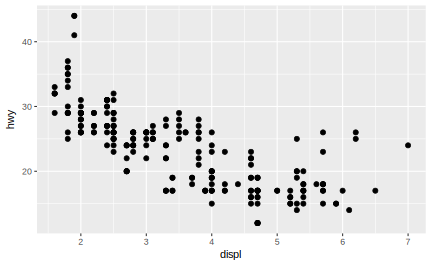
\includegraphics{img/ggplot2/basic_mpg-1.pdf}

To walk through the above code:

\begin{itemize}
\item
  The \texttt{ggplot()} function is passed the data frame to plot as the
  \texttt{data} argument.
\item
  You specify a geometric object (\texttt{geom}) by calling one of the
  many\texttt{geom}
  \href{http://ggplot2.tidyverse.org/reference/index.html\#section-layer-geoms}{functions},
  which are all named \texttt{geom\_} followed by the name of the kind
  of geometry you wish to create. For example, \texttt{geom\_point()}
  will create a layer with ``point'' (dot) elements as the geometry.
  There are large number of these functions; see below for more details.
\item
  For each \texttt{geom} you must specify the \textbf{aesthetic
  mappings}, which is how data from the data frame will be mapped to the
  visual aspects of the geometry. These mappings are defined using the
  \texttt{aes()} function. The \texttt{aes()} function takes a set of
  arguments (like a list), where the argument name is the visual
  property to map \emph{to}, and the argument value is the data property
  to map \emph{from}.
\item
  Finally, you add \texttt{geom} layers to the plot by using the
  addition (\textbf{\texttt{+}}) operator.
\end{itemize}

Thus basic simple plots can be created simply by specifying a data set,
a \texttt{geom}, and a set of aesthetic mappings.

\begin{itemize}
\tightlist
\item
  Note that \texttt{ggplot2} library does include a \texttt{qlot()}
  function for creating ``quick plots'', which acts as a convenient
  shortcut for making simple, ``default''-like plots. However, for this
  course you should focus on thinking about plots in terms of the
  \emph{Grammar of Graphics} and use the \texttt{ggplot()} function
  instead.
\end{itemize}

\subsection{Aesthetic Mappings}\label{aesthetic-mappings}

The \textbf{aesthetic mappings} take properties of the data and use them
to influence \textbf{visual channels}, such as \emph{position},
\emph{color}, \emph{size}, or \emph{shape}. Each visual channel can thus
encode an aspect of the data and be used to convey information.

All aesthetics for a plot are specified in the
\href{http://ggplot2.tidyverse.org/reference/index.html\#section-aesthetics}{\texttt{aes()}}
function call for that \texttt{geom} layer. For example, you can add a
mapping from the \texttt{class} of the cars to the \emph{color} channel:

\begin{Shaded}
\begin{Highlighting}[]
\CommentTok{# color the data by car type}
\KeywordTok{ggplot}\NormalTok{(}\DataTypeTok{data =}\NormalTok{ mpg) }\OperatorTok{+}
\StringTok{  }\KeywordTok{geom_point}\NormalTok{(}\DataTypeTok{mapping =} \KeywordTok{aes}\NormalTok{(}\DataTypeTok{x =}\NormalTok{ displ, }\DataTypeTok{y =}\NormalTok{ hwy, }\DataTypeTok{color =}\NormalTok{ class))}
\end{Highlighting}
\end{Shaded}

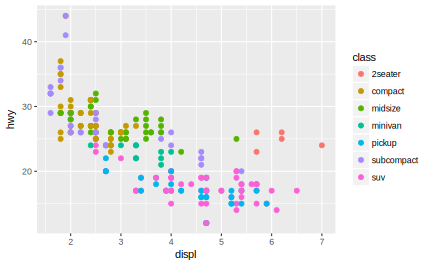
\includegraphics{img/ggplot2/aes_color-1.pdf}

(\texttt{ggplot2} will even create a legend for you!)

Note that using the \texttt{aes()} function will cause the visual
channel to be based on the data specified in the argument. For example,
using \texttt{aes(color\ =\ "blue")} won't cause the geometry's color to
be ``blue'', but will instead cause the visual channel to be mapped from
the \emph{vector} \texttt{c("blue")}---as if you only had a single type
of engine that happened to be called ``blue''. If you wish to apply an
aesthetic property to an entire geometry, you can \textbf{\emph{set}}
that property as an argument to the \texttt{geom} method, outside of the
\texttt{aes()} call:

\begin{Shaded}
\begin{Highlighting}[]
\KeywordTok{ggplot}\NormalTok{(}\DataTypeTok{data =}\NormalTok{ mpg) }\OperatorTok{+}\StringTok{                         }\CommentTok{# note where parentheses are closed}
\StringTok{  }\KeywordTok{geom_point}\NormalTok{(}\DataTypeTok{mapping =} \KeywordTok{aes}\NormalTok{(}\DataTypeTok{x =}\NormalTok{ displ, }\DataTypeTok{y =}\NormalTok{ hwy), }\DataTypeTok{color =} \StringTok{"blue"}\NormalTok{)  }\CommentTok{# blue points!}
\end{Highlighting}
\end{Shaded}

\includegraphics{img/ggplot2/color_blue-1.pdf}

\section{Complex Plots}\label{complex-plots}

Building on these basics, \texttt{ggplot2} can be used to build almost
any kind of plot you may want. These plots are declared using functions
that follow from the \emph{Grammar of Graphics}.

\subsection{Specifying Geometry}\label{specifying-geometry}

The most obvious distinction between plots is what \textbf{geometric
objects} (\texttt{geoms}) they include. \texttt{ggplot2} supports a
number of different types of
\href{http://ggplot2.tidyverse.org/reference/index.html\#section-layer-geoms}{\texttt{geoms}},
including:

\begin{itemize}
\tightlist
\item
  \textbf{\texttt{geom\_point}} for drawing individual points (e.g., a
  scatter plot)
\item
  \textbf{\texttt{geom\_line}} for drawing lines (e.g., for a line
  charts)
\item
  \textbf{\texttt{geom\_smooth}} for drawing smoothed lines (e.g., for
  simple trends or approximations)
\item
  \textbf{\texttt{geom\_bar}} for drawing bars (e.g., for bar charts)
\item
  \textbf{\texttt{geom\_polygon}} for drawing arbitrary shapes
\item
  \textbf{\texttt{geom\_map}} for drawing polygons in the shape of a
  map! (You can access the \emph{data} to use for these maps by using
  the
  \href{http://ggplot2.tidyverse.org/reference/map_data.html}{\texttt{map\_data()}}
  function).
\end{itemize}

Each of these geometries will need to include a set of \textbf{aesthetic
mappings} (using the \texttt{aes()} function and assigned to the
\texttt{mapping} argument), though the specific \emph{visual properties}
that the data will map to will vary. For example, you can map data to
the \texttt{shape} of a \texttt{geom\_point} (e.g., if they should be
circles or squares), or you can map data to the \texttt{linetype} of a
\texttt{geom\_line} (e.g., if it is solid or dotted), but not vice
versa.

\begin{itemize}
\tightlist
\item
  Almost all \texttt{geoms} \textbf{require} an \texttt{x} and
  \texttt{y} mapping at the bare minimum.
\end{itemize}

\begin{Shaded}
\begin{Highlighting}[]
\CommentTok{# line chart of milage by engine power}
\KeywordTok{ggplot}\NormalTok{(}\DataTypeTok{data =}\NormalTok{ mpg) }\OperatorTok{+}
\StringTok{  }\KeywordTok{geom_line}\NormalTok{(}\DataTypeTok{mapping =} \KeywordTok{aes}\NormalTok{(}\DataTypeTok{x =}\NormalTok{ displ, }\DataTypeTok{y =}\NormalTok{ hwy))}

\CommentTok{# bar chart of car type}
\KeywordTok{ggplot}\NormalTok{(}\DataTypeTok{data =}\NormalTok{ mpg) }\OperatorTok{+}
\StringTok{  }\KeywordTok{geom_bar}\NormalTok{(}\DataTypeTok{mapping =} \KeywordTok{aes}\NormalTok{(}\DataTypeTok{x =}\NormalTok{ class))  }\CommentTok{# no y mapping needed!}
\end{Highlighting}
\end{Shaded}

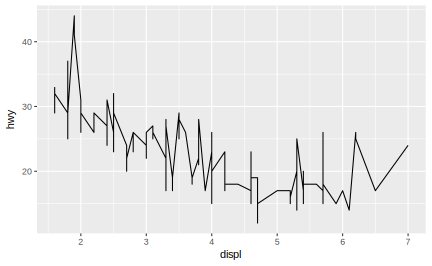
\includegraphics[width=380pt]{img/ggplot2/geom_examples-1}
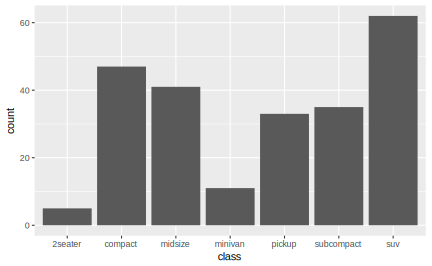
\includegraphics[width=380pt]{img/ggplot2/geom_examples-2}

What makes this really powerful is that you can add \textbf{multiple
geometries} to a plot, thus allowing you to create complex graphics
showing multiple aspects of your data

\begin{Shaded}
\begin{Highlighting}[]
\CommentTok{# plot with both points and smoothed line}
\KeywordTok{ggplot}\NormalTok{(}\DataTypeTok{data =}\NormalTok{ mpg) }\OperatorTok{+}
\StringTok{  }\KeywordTok{geom_point}\NormalTok{(}\DataTypeTok{mapping =} \KeywordTok{aes}\NormalTok{(}\DataTypeTok{x =}\NormalTok{ displ, }\DataTypeTok{y =}\NormalTok{ hwy)) }\OperatorTok{+}
\StringTok{  }\KeywordTok{geom_smooth}\NormalTok{(}\DataTypeTok{mapping =} \KeywordTok{aes}\NormalTok{(}\DataTypeTok{x =}\NormalTok{ displ, }\DataTypeTok{y =}\NormalTok{ hwy))}
\end{Highlighting}
\end{Shaded}

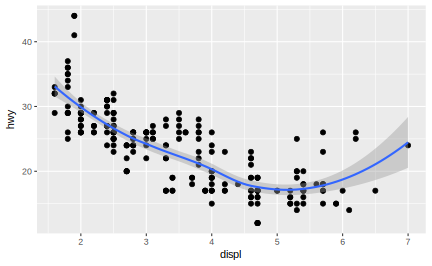
\includegraphics{img/ggplot2/multi_geom-1.pdf}

Of course the aesthetics for each \texttt{geom} can be different, so you
could show multiple lines on the same plot (or with different colors,
styles, etc). It's also possible to give each \texttt{geom} a different
\texttt{data} argument, so that you can show multiple data sets in the
same plot.

\begin{itemize}
\tightlist
\item
  If you want multiple \texttt{geoms} to utilize the same data or
  aesthetics, you can pass those values as arguments to the
  \texttt{ggplot()} function itself; any \texttt{geoms} added to that
  plot will use the values declared for the whole plot \emph{unless
  overridden by individual specifications}.
\end{itemize}

\subsubsection{Statistical
Transformations}\label{statistical-transformations}

If you look at the above \texttt{bar} chart, you'll notice that the the
\texttt{y} axis was defined for you as the \texttt{count} of elements
that have the particular type. This \texttt{count} isn't part of the
data set (it's not a column in \texttt{mpg}), but is instead a
\textbf{statistical transformation} that the \texttt{geom\_bar}
automatically applies to the data. In particular, it applies the
\texttt{stat\_count} transformation.

\texttt{ggplot2} supports many different statistical transformations.
For example, the ``identity'' transformation will leave the data ``as
is''. You can specify which statistical transformation a \texttt{geom}
uses by passing it as the \textbf{\texttt{stat}} argument:

\begin{Shaded}
\begin{Highlighting}[]
\CommentTok{# silly example: bar chart of engine power vs. milage}
\CommentTok{# (you need the `y` mapping since it is not implied by the stat transform}
\KeywordTok{ggplot}\NormalTok{(}\DataTypeTok{data =}\NormalTok{ mpg) }\OperatorTok{+}
\StringTok{  }\KeywordTok{geom_bar}\NormalTok{(}\DataTypeTok{mapping =} \KeywordTok{aes}\NormalTok{(}\DataTypeTok{x =}\NormalTok{ displ, }\DataTypeTok{y =}\NormalTok{ hwy), }\DataTypeTok{stat=}\StringTok{"identity"}\NormalTok{)}
\end{Highlighting}
\end{Shaded}

Additionally, \texttt{ggplot2} contains \textbf{\texttt{stat\_}}
functions (e.g., \texttt{stat\_identity} for the ``identity''
transformation) that can be used to specify a layer in the same way a
\texttt{geom} does:

\begin{Shaded}
\begin{Highlighting}[]
\CommentTok{# generate a "binned" (grouped) display of highway milage}
\KeywordTok{ggplot}\NormalTok{(}\DataTypeTok{data =}\NormalTok{ mpg) }\OperatorTok{+}
\StringTok{  }\KeywordTok{stat_bin}\NormalTok{(}\KeywordTok{aes}\NormalTok{(}\DataTypeTok{x=}\NormalTok{hwy, }\DataTypeTok{color=}\NormalTok{hwy), }\DataTypeTok{binwidth=}\DecValTok{4}\NormalTok{)  }\CommentTok{# binned into groups of 4 units}
\end{Highlighting}
\end{Shaded}

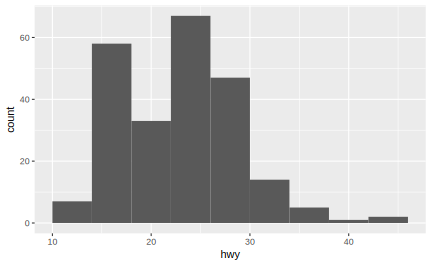
\includegraphics{img/ggplot2/stat_summary-1.pdf}

Notice the above chart is actually a
\href{https://en.wikipedia.org/wiki/Histogram}{histogram}! Indeed,
almost every \texttt{stat} transformation corresponds to a particular
\texttt{geom} (and vice versa) by default. Thus they can often be used
interchangeably, depending on how you want to emphasize your layer
creation when writing the code.

\begin{Shaded}
\begin{Highlighting}[]
\CommentTok{# these two charts are identical}
\KeywordTok{ggplot}\NormalTok{(}\DataTypeTok{data =}\NormalTok{ mpg) }\OperatorTok{+}
\StringTok{  }\KeywordTok{geom_bar}\NormalTok{(}\DataTypeTok{mapping =} \KeywordTok{aes}\NormalTok{(}\DataTypeTok{x =}\NormalTok{ class))}

\KeywordTok{ggplot}\NormalTok{(}\DataTypeTok{data =}\NormalTok{ mpg) }\OperatorTok{+}
\StringTok{  }\KeywordTok{stat_count}\NormalTok{(}\DataTypeTok{mapping =} \KeywordTok{aes}\NormalTok{(}\DataTypeTok{x =}\NormalTok{ class))}
\end{Highlighting}
\end{Shaded}

\subsubsection{Position Adjustments}\label{position-adjustments}

In addition to a default statistical transformation, each \texttt{geom}
also has a default \textbf{position adjustment} which specifies a set of
``rules'' as to how different components should be positioned relative
to each other. This position is noticeable in a \texttt{geom\_bar} if
you map a different variable to the color visual channel:

\begin{Shaded}
\begin{Highlighting}[]
\CommentTok{# bar chart of milage, colored by engine type}
\KeywordTok{ggplot}\NormalTok{(}\DataTypeTok{data =}\NormalTok{ mpg) }\OperatorTok{+}
\StringTok{  }\KeywordTok{geom_bar}\NormalTok{(}\DataTypeTok{mapping =} \KeywordTok{aes}\NormalTok{(}\DataTypeTok{x =}\NormalTok{ hwy, }\DataTypeTok{fill=}\NormalTok{class))  }\CommentTok{# fill color, not outline color}
\end{Highlighting}
\end{Shaded}

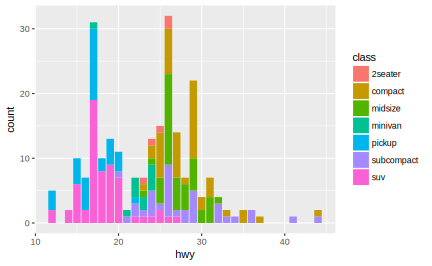
\includegraphics{img/ggplot2/stacked_bar-1.pdf}

The \texttt{geom\_bar} by default uses a position adjustment of
\texttt{"stack"}, which makes each ``bar'' a height appropriate to its
value and \emph{stacks} them on top of each other. You can use the
\textbf{\texttt{position}} argument to specify what position adjustment
rules to follow:

\begin{Shaded}
\begin{Highlighting}[]
\CommentTok{# a filled bar chart (fill the vertical height)}
\KeywordTok{ggplot}\NormalTok{(}\DataTypeTok{data =}\NormalTok{ mpg) }\OperatorTok{+}
\StringTok{  }\KeywordTok{geom_bar}\NormalTok{(}\DataTypeTok{mapping =} \KeywordTok{aes}\NormalTok{(}\DataTypeTok{x =}\NormalTok{ hwy, }\DataTypeTok{fill=}\NormalTok{drv), }\DataTypeTok{position=}\StringTok{"fill"}\NormalTok{)}

\CommentTok{# a dodged bar chart (values next to each other)}
\CommentTok{# (not great dodging demos in this data set)}
\KeywordTok{ggplot}\NormalTok{(}\DataTypeTok{data =}\NormalTok{ mpg) }\OperatorTok{+}
\StringTok{  }\KeywordTok{geom_bar}\NormalTok{(}\DataTypeTok{mapping =} \KeywordTok{aes}\NormalTok{(}\DataTypeTok{x =}\NormalTok{ hwy, }\DataTypeTok{fill=}\NormalTok{drv), }\DataTypeTok{position=}\StringTok{"dodge"}\NormalTok{)}
\end{Highlighting}
\end{Shaded}

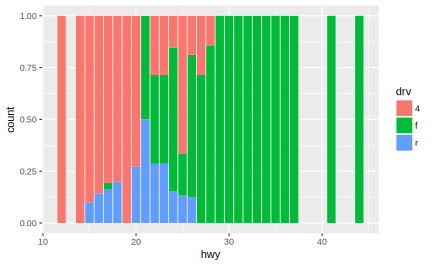
\includegraphics[width=380pt]{img/ggplot2/position_examples-1}
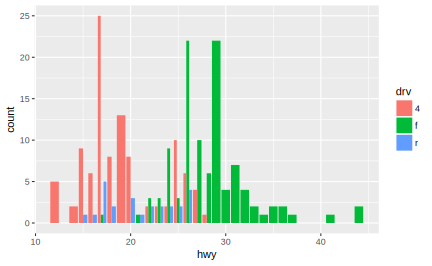
\includegraphics[width=380pt]{img/ggplot2/position_examples-2}

Check the documentation for each particular \texttt{geom} to learn more
about its possible position adjustments.

\subsection{Styling with Scales}\label{styling-with-scales}

Whenever you specify an \textbf{aesthetic mapping}, \texttt{ggplot} uses
a particular \textbf{scale} to determine the \emph{range of values} that
the data should map to. Thus when you specify

\begin{Shaded}
\begin{Highlighting}[]
\CommentTok{# color the data by engine type}
\KeywordTok{ggplot}\NormalTok{(}\DataTypeTok{data =}\NormalTok{ mpg) }\OperatorTok{+}
\StringTok{  }\KeywordTok{geom_point}\NormalTok{(}\DataTypeTok{mapping =} \KeywordTok{aes}\NormalTok{(}\DataTypeTok{x =}\NormalTok{ displ, }\DataTypeTok{y =}\NormalTok{ hwy, }\DataTypeTok{color =}\NormalTok{ class))}
\end{Highlighting}
\end{Shaded}

\texttt{ggplot} automatically adds a \textbf{scale} for each mapping to
the plot:

\begin{Shaded}
\begin{Highlighting}[]
\CommentTok{# same as above, with explicit scales}
\KeywordTok{ggplot}\NormalTok{(}\DataTypeTok{data =}\NormalTok{ mpg) }\OperatorTok{+}
\StringTok{  }\KeywordTok{geom_point}\NormalTok{(}\DataTypeTok{mapping =} \KeywordTok{aes}\NormalTok{(}\DataTypeTok{x =}\NormalTok{ displ, }\DataTypeTok{y =}\NormalTok{ hwy, }\DataTypeTok{color =}\NormalTok{ class)) }\OperatorTok{+}
\StringTok{  }\KeywordTok{scale_x_continuous}\NormalTok{() }\OperatorTok{+}
\StringTok{  }\KeywordTok{scale_y_continuous}\NormalTok{() }\OperatorTok{+}
\StringTok{  }\KeywordTok{scale_colour_discrete}\NormalTok{()}
\end{Highlighting}
\end{Shaded}

Each scale can be represented by a function with the following name:
\texttt{scale\_}, followed by the name of the aesthetic property,
followed by an \texttt{\_} and the name of the scale. A
\texttt{continuous} scale will handle things like numeric data (where
there is a \emph{continuous set} of numbers), whereas a
\texttt{discrete} scale will handle things like colors (since there is a
small list of \emph{distinct} colors).

While the default scales will work fine, it is possible to explicitly
add different scales to replace the defaults. For example, you can use a
scale to change the direction of an axis:

\begin{Shaded}
\begin{Highlighting}[]
\CommentTok{# milage relationship, ordered in reverse}
\KeywordTok{ggplot}\NormalTok{(}\DataTypeTok{data =}\NormalTok{ mpg) }\OperatorTok{+}
\StringTok{  }\KeywordTok{geom_point}\NormalTok{(}\DataTypeTok{mapping =} \KeywordTok{aes}\NormalTok{(}\DataTypeTok{x =}\NormalTok{ cty, }\DataTypeTok{y =}\NormalTok{ hwy)) }\OperatorTok{+}
\StringTok{  }\KeywordTok{scale_x_reverse}\NormalTok{()}
\end{Highlighting}
\end{Shaded}

Similarly, you can use \texttt{scale\_x\_log10()} to plot on a
\href{https://en.wikipedia.org/wiki/Logarithmic_scale}{logarithmic
scale}.

You can also use scales to specify the \emph{range} of values on a axis
by passing in a \texttt{limits} argument. This is useful for making sure
that multiple graphs share scales or formats.

\begin{Shaded}
\begin{Highlighting}[]
\CommentTok{# subset data by class}
\NormalTok{suv =}\StringTok{ }\NormalTok{mpg }\OperatorTok\StringTok{ }\KeywordTok{filter}\NormalTok{(class }\OperatorTok{==}\StringTok{ "suv"}\NormalTok{)  }\CommentTok{# suvs}
\NormalTok{compact =}\StringTok{ }\NormalTok{mpg }\OperatorTok\StringTok{ }\KeywordTok{filter}\NormalTok{(class }\OperatorTok{==}\StringTok{ "compact"}\NormalTok{)  }\CommentTok{# compact cars}

\CommentTok{# scales}
\NormalTok{x_scale <-}\StringTok{ }\KeywordTok{scale_x_continuous}\NormalTok{(}\DataTypeTok{limits =} \KeywordTok{range}\NormalTok{(mpg}\OperatorTok{$}\NormalTok{displ))}
\NormalTok{y_scale <-}\StringTok{ }\KeywordTok{scale_y_continuous}\NormalTok{(}\DataTypeTok{limits =} \KeywordTok{range}\NormalTok{(mpg}\OperatorTok{$}\NormalTok{hwy))}
\NormalTok{col_scale <-}\StringTok{ }\KeywordTok{scale_colour_discrete}\NormalTok{(}\DataTypeTok{limits =} \KeywordTok{unique}\NormalTok{(mpg}\OperatorTok{$}\NormalTok{drv))}

\KeywordTok{ggplot}\NormalTok{(}\DataTypeTok{data =}\NormalTok{ suv) }\OperatorTok{+}
\StringTok{  }\KeywordTok{geom_point}\NormalTok{(}\DataTypeTok{mapping =} \KeywordTok{aes}\NormalTok{(}\DataTypeTok{x =}\NormalTok{ displ, }\DataTypeTok{y =}\NormalTok{ hwy, }\DataTypeTok{color =}\NormalTok{ drv)) }\OperatorTok{+}
\StringTok{  }\NormalTok{x_scale }\OperatorTok{+}\StringTok{ }\NormalTok{y_scale }\OperatorTok{+}\StringTok{ }\NormalTok{col_scale}

\KeywordTok{ggplot}\NormalTok{(}\DataTypeTok{data =}\NormalTok{ compact) }\OperatorTok{+}
\StringTok{  }\KeywordTok{geom_point}\NormalTok{(}\DataTypeTok{mapping =} \KeywordTok{aes}\NormalTok{(}\DataTypeTok{x =}\NormalTok{ displ, }\DataTypeTok{y =}\NormalTok{ hwy, }\DataTypeTok{color =}\NormalTok{ drv)) }\OperatorTok{+}
\StringTok{  }\NormalTok{x_scale }\OperatorTok{+}\StringTok{ }\NormalTok{y_scale }\OperatorTok{+}\StringTok{ }\NormalTok{col_scale}
\end{Highlighting}
\end{Shaded}

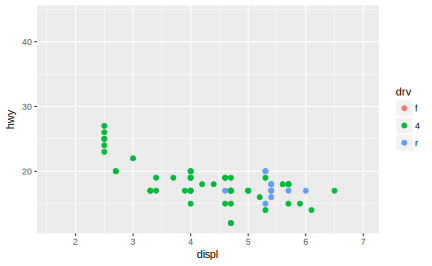
\includegraphics[width=380pt]{img/ggplot2/scale_limit-1}
\includegraphics[width=380pt]{img/ggplot2/scale_limit-2}

Notice how it is easy to compare the two data sets to each other because
the axes and colors match!

These scales can also be used to specify the ``tick'' marks and labels;
see the resources at the end of the chapter for details. And for further
ways specifying where the data appears on the graph, see the
\protect\hyperlink{coordinate-systems}{Coordinate Systems} section
below.

\subsubsection{Color Scales}\label{color-scales}

A more common scale to change is which set of colors to use in a plot.
While you can use scale functions to specify a list of colors to use, a
more common option is to use a pre-defined palette from
\href{http://colorbrewer2.org/}{\textbf{colorbrewer.org}}. These color
sets have been carefully designed to look good and to be viewable to
people with certain forms of color blindness. This color scale is
specified with the \texttt{scale\_color\_brewer()} function, passing the
\texttt{palette} as an argument.

\begin{Shaded}
\begin{Highlighting}[]
\KeywordTok{ggplot}\NormalTok{(}\DataTypeTok{data =}\NormalTok{ mpg) }\OperatorTok{+}
\StringTok{  }\KeywordTok{geom_point}\NormalTok{(}\DataTypeTok{mapping =} \KeywordTok{aes}\NormalTok{(}\DataTypeTok{x =}\NormalTok{ displ, }\DataTypeTok{y =}\NormalTok{ hwy, }\DataTypeTok{color =}\NormalTok{ class), }\DataTypeTok{size=}\DecValTok{4}\NormalTok{) }\OperatorTok{+}
\StringTok{  }\KeywordTok{scale_color_brewer}\NormalTok{(}\DataTypeTok{palette =} \StringTok{"Set3"}\NormalTok{)}
\end{Highlighting}
\end{Shaded}

\includegraphics{img/ggplot2/brewer_point-1.pdf}

You can get the palette name from the \emph{colorbrewer} website by
looking at the \texttt{scheme} query parameter in the URL. Or see the
diagram \href{https://bl.ocks.org/mbostock/5577023}{here} and hover the
mouse over each palette for its name.

You can also specify \emph{continuous} color values by using a
\href{http://ggplot2.tidyverse.org/reference/scale_gradient.html}{gradient}
scale, or
\href{http://ggplot2.tidyverse.org/reference/scale_manual.html}{manually}
specify the colors you want to use as a \emph{named vector}.

\hypertarget{coordinate-systems}{\subsection{Coordinate
Systems}\label{coordinate-systems}}

The next term from the \emph{Grammar of Graphics} that can be specified
is the \textbf{coordinate system}. As with \textbf{scales}, coordinate
systems are specified with functions (that all start with
\textbf{\texttt{coord\_}}) and are added to a \texttt{ggplot}. There are
a number of different possible
\href{http://ggplot2.tidyverse.org/reference/index.html\#section-coordinate-systems}{coordinate
systems} to use, including:

\begin{itemize}
\tightlist
\item
  \textbf{\texttt{coord\_cartesian}} the default
  \href{https://en.wikipedia.org/wiki/Cartesian_coordinate_system}{cartesian
  coordinate} system, where you specify \texttt{x} and \texttt{y}
  values.
\item
  \textbf{\texttt{coord\_flip}} a cartesian system with the \texttt{x}
  and \texttt{y} flipped
\item
  \textbf{\texttt{coord\_fixed}} a cartesian system with a ``fixed''
  aspect ratio (e.g., 1.78 for a ``widescreen'' plot)
\item
  \textbf{\texttt{coord\_polar}} a plot using
  \href{https://en.wikipedia.org/wiki/Polar_coordinate_system}{polar
  coordinates}
\item
  \textbf{\texttt{coord\_quickmap}} a coordinate system that
  approximates a good aspect ratio for maps. See the documentation for
  more details.
\end{itemize}

Most of these system support the \texttt{xlim} and \texttt{ylim}
arguments, which specify the \emph{limits} for the coordinate system.

\subsection{Facets}\label{facets}

\textbf{Facets} are ways of \emph{grouping} a data plot into multiple
different pieces (\emph{subplots}). This allows you to view a separate
plot for each value in a
\href{https://en.wikipedia.org/wiki/Categorical_variable}{categorical
variable}. Conceptually, breaking a plot up into facets is similar to
using the \texttt{group\_by()} verb in \texttt{dplyr}, with each facet
acting like a \emph{level} in an R \emph{factor}.

You can construct a plot with multiple facets by using the
\textbf{\texttt{facet\_wrap()}} function. This will produce a ``row'' of
subplots, one for each categorical variable (the number of rows can be
specified with an additional argument):

\begin{Shaded}
\begin{Highlighting}[]
\CommentTok{# a plot with facets based on vehicle type.}
\CommentTok{# similar to what we did with `suv` and `compact`!}
\KeywordTok{ggplot}\NormalTok{(}\DataTypeTok{data =}\NormalTok{ mpg) }\OperatorTok{+}
\StringTok{  }\KeywordTok{geom_point}\NormalTok{(}\DataTypeTok{mapping =} \KeywordTok{aes}\NormalTok{(}\DataTypeTok{x =}\NormalTok{ displ, }\DataTypeTok{y =}\NormalTok{ hwy)) }\OperatorTok{+}
\StringTok{  }\KeywordTok{facet_wrap}\NormalTok{(}\OperatorTok{~}\NormalTok{class)}
\end{Highlighting}
\end{Shaded}

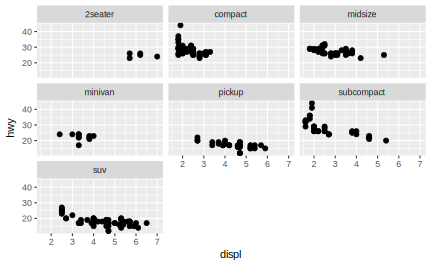
\includegraphics{img/ggplot2/facets-1.pdf}

Note that the argument to \texttt{facet\_wrap()} function is written
with a tilde (\textbf{\texttt{\textasciitilde{}}}) in front of it. This
specifies that the column name should be treated as a \textbf{formula}.
A formula is a bit like an ``equation'' in mathematics; it's like a
string representing what set of operations you want to perform (putting
the column name in a string also works in this simple case). Formulas
are in fact the same structure used with \emph{standard evaluation} in
\texttt{dplyr}; putting a \texttt{\textasciitilde{}} in front of an
expression (such as \texttt{\textasciitilde{}\ desc(colname)}) allows SE
to work.

\begin{itemize}
\tightlist
\item
  In short: put a \texttt{\textasciitilde{}} in front of the column name
  you want to ``group'' by.
\end{itemize}

\subsection{Labels \& Annotations}\label{labels-annotations}

Textual labels and annotations (on the plot, axes, geometry, and legend)
are an important part of making a plot understandable and communicating
information. Although not an explicit part of the \emph{Grammar of
Graphics} (they would be considered a form of geometry), \texttt{ggplot}
makes it easy to add such annotations.

You can add titles and axis labels to a chart using the
\textbf{\texttt{labs()}} function (\emph{not} \texttt{labels}, which is
a different R function!):

\begin{Shaded}
\begin{Highlighting}[]
\KeywordTok{ggplot}\NormalTok{(}\DataTypeTok{data =}\NormalTok{ mpg) }\OperatorTok{+}
\StringTok{  }\KeywordTok{geom_point}\NormalTok{(}\DataTypeTok{mapping =} \KeywordTok{aes}\NormalTok{(}\DataTypeTok{x =}\NormalTok{ displ, }\DataTypeTok{y =}\NormalTok{ hwy, }\DataTypeTok{color =}\NormalTok{ class)) }\OperatorTok{+}
\StringTok{  }\KeywordTok{labs}\NormalTok{(}\DataTypeTok{title =} \StringTok{"Fuel Efficiency by Engine Power, 1999-2008"}\NormalTok{,  }\CommentTok{# plot title}
       \DataTypeTok{x =} \StringTok{"Engine power (litres displacement)"}\NormalTok{,  }\CommentTok{# x-axis label (with units!)}
       \DataTypeTok{y =} \StringTok{"Fuel Efficiency (miles per gallon)"}\NormalTok{,  }\CommentTok{# y-axis label (with units!)}
       \DataTypeTok{color =} \StringTok{"Car Type"}\NormalTok{)  }\CommentTok{# legend label for the "color" property}
\end{Highlighting}
\end{Shaded}

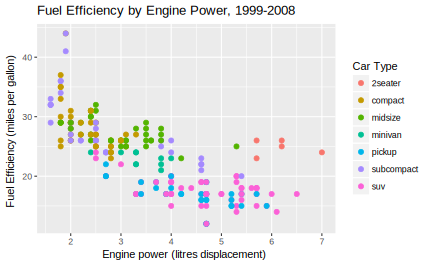
\includegraphics{img/ggplot2/labels-1.pdf}

It is possible to add labels into the plot itself (e.g., to label each
point or line) by adding a new \texttt{geom\_text} or
\texttt{geom\_label} to the plot; effectively, you're plotting an extra
set of data which happen to be the variable names:

\begin{Shaded}
\begin{Highlighting}[]
\CommentTok{# a data table of each car that has best efficiency of its type}
\NormalTok{best_in_class <-}\StringTok{ }\NormalTok{mpg }\OperatorTok
\StringTok{  }\KeywordTok{group_by}\NormalTok{(class) }\OperatorTok
\StringTok{  }\KeywordTok{filter}\NormalTok{(}\KeywordTok{row_number}\NormalTok{(}\KeywordTok{desc}\NormalTok{(hwy)) }\OperatorTok{==}\StringTok{ }\DecValTok{1}\NormalTok{)}

\KeywordTok{ggplot}\NormalTok{(}\DataTypeTok{data =}\NormalTok{ mpg, }\DataTypeTok{mapping =} \KeywordTok{aes}\NormalTok{(}\DataTypeTok{x =}\NormalTok{ displ, }\DataTypeTok{y =}\NormalTok{ hwy)) }\OperatorTok{+}\StringTok{  }\CommentTok{# same mapping for all geoms}
\StringTok{  }\KeywordTok{geom_point}\NormalTok{(}\DataTypeTok{mapping =} \KeywordTok{aes}\NormalTok{(}\DataTypeTok{color =}\NormalTok{ class)) }\OperatorTok{+}
\StringTok{  }\KeywordTok{geom_label}\NormalTok{(}\DataTypeTok{data =}\NormalTok{ best_in_class, }\DataTypeTok{mapping =} \KeywordTok{aes}\NormalTok{(}\DataTypeTok{label =}\NormalTok{ model), }\DataTypeTok{alpha =} \FloatTok{0.5}\NormalTok{)}
\end{Highlighting}
\end{Shaded}

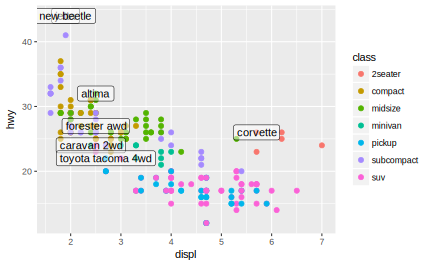
\includegraphics{img/ggplot2/annotations-1.pdf}

\emph{R for Data Science} (linked in the resources below) recommends
using the \href{https://github.com/slowkow/ggrepel}{\texttt{ggrepel}}
package to help position labels.

\section{Other Visualization
Libraries}\label{other-visualization-libraries}

\texttt{ggplot2} is easily the most popular library for producing data
visualizations in R. That said, \texttt{ggplot2} is used to produce
\textbf{static} visualizations: unchanging ``pictures'' of plots. Static
plots are great for for \textbf{explanatory visualizations}:
visualizations that are used to communicate some information---or more
commonly, an \emph{argument} about that information. All of the above
visualizations have been ways to explain and demonstrate an argument
about the data (e.g., the relationship between car engines and fuel
efficiency).

Data visualizations can also be highly effective for \textbf{exploratory
analysis}, in which the visualization is used as a way to \emph{ask and
answer questions} about the data (rather than to convey an answer or
argument). While it is perfectly feasible to do such exploration on a
static visualization, many explorations can be better served with
\textbf{interactive visualizations} in which the user can select and
change the \emph{view} and presentation of that data in order to
understand it.

While \texttt{ggplot2} does not directly support interactive
visualizations, there are a number of additional R libraries that
provide this functionality, including:

\begin{itemize}
\item
  \href{http://ggvis.rstudio.com/}{\textbf{\texttt{ggvis}}} is a library
  that uses the \emph{Grammar of Graphics} (similar to \texttt{ggplot}),
  but for interactive visualizations. The interactivity is provided
  through the \href{http://www.rstudio.com/shiny/}{\texttt{shiny}}
  library, which is introduced in a later chapter.
\item
  \href{http://hafen.github.io/rbokeh/index.html}{\textbf{Bokeh}} is an
  open-source library for developing interactive visualizations. It
  automatically provides a number of ``standard'' interactions (pop-up
  labels, drag to pan, select to zoom, etc) automatically. It is similar
  to \texttt{ggplot2}, in that you create a figure and then and then add
  \emph{layers} representing different geometries (points, lines etc).
  It has detailed and readable documentation, and is also available to
  other programming languages (such as Python).
\item
  \href{https://plot.ly/r/}{\textbf{Plotly}} is another libary similar
  to \emph{Bokeh}, in that it automatically provided standard
  interactions. It is also possible to take a \texttt{ggplot2} plot and
  \href{https://plot.ly/ggplot2/}{wrap} it in Plotly in order to make it
  interactive. Plotly has many examples to learn from, though a less
  effective set of documentation than other libraries.
\item
  \href{http://rdatascience.io/rCharts/}{\textbf{\texttt{rCharts}}}
  provides a way to utilize a number of \emph{JavaScript} interactive
  visualization libraries. JavaScript is the programming language used
  to create interactive websites (HTML files), and so is highly
  specialized for creating interactive experiences.
\end{itemize}

There are many other libraries as well; searching around for a specific
feature you need may lead you to a useful tool!

\section*{Resources}\label{resources-12}


\begin{itemize}
\tightlist
\item
  \href{http://ggplot2.tidyverse.org/}{gglot2 Documentation}
  (particularly the
  \href{http://ggplot2.tidyverse.org/reference/index.html}{function
  reference})
\item
  \href{https://www.rstudio.com/wp-content/uploads/2016/11/ggplot2-cheatsheet-2.1.pdf}{ggplot2
  Cheat Sheet} (see also
  \href{http://zevross.com/blog/2014/08/04/beautiful-plotting-in-r-a-ggplot2-cheatsheet-3/}{here})
\item
  \href{http://r4ds.had.co.nz/data-visualisation.html}{Data
  Visualization (R4DS)} - tutorial using \texttt{ggplot2}
\item
  \href{http://r4ds.had.co.nz/graphics-for-communication.html}{Graphics
  for Communication (R4DS)} - ``part 2'' of tutorial using
  \texttt{ggplot}
\item
  \href{http://www.statmethods.net/advgraphs/ggplot2.html}{Graphics with
  ggplot2} - explanation of \texttt{qplot()}
\item
  \href{https://codewords.recurse.com/issues/six/telling-stories-with-data-using-the-grammar-of-graphics}{Telling
  stories with the grammar of graphics}
\item
  \href{http://vita.had.co.nz/papers/layered-grammar.pdf}{A Layered
  Grammar of Graphics (Wickham)}
\end{itemize}

\hypertarget{git-branches}{\chapter{Git Branches and
Collaboration}\label{git-branches}}

While \texttt{git} is great for uploading and downloading code, its true
benefits are its ability to support \emph{reversability} (e.g., undo)
and \emph{collaboration} (working with other people). In order to
effectively utilize these capabilities, you need to understand git's
\textbf{branching model}, which is central to how the program manages
different versions of code.

This chapter will cover how to work with \textbf{branches} with git and
GitHub, including using them to work on different features
simultaneously and to undo previous changes. It will also discuss how to
use branches to support different \emph{collaborative workflows},
allowing multiple people to work on code in the same repository.

\hypertarget{git-branches}{\section{Git Branches}\label{git-branches}}

So far, you've been using git to create a \emph{linear sequence} of
commits: they are all in a line, one after another).

Each commit has a message associated with it (that you can see with
\texttt{git\ log\ -\/-online}), as well as a unique
\href{https://en.wikipedia.org/wiki/SHA-1}{SHA-1} hash (the random
numbers and letters), which can be used to identify that commit as an
``id number''.

But you can also save commits in a \emph{non-linear} sequence. Perhaps
you want to try something new and crazy without breaking code that
you've already written. Or you want to work on two different features
simultaneously (having separate commits for each). Or you want multiple
people to work on the same code without stepping on each other's toes.

To do this, you use a feature of git called \textbf{branching} (because
you can have commits that ``branch off'' from a line of development):

In this example, you have a primary branch (called the \texttt{master}
branch), and decide you want to try an experiment. You \emph{split off}
a new branch (called for example \texttt{experiment}), which saves some
funky changes to your code. But then you decide to make further changes
to your main development line, adding more commits to \texttt{master}
that ignore the changes stored in the \texttt{experiment} branch. You
can develop \texttt{master} and \texttt{experiment} simultaneously,
making changes to each version of the code. You can even branch off
further versions (e.g., a \texttt{bugfix} to fix a problem) if you wish.
And once you decide you're happy with the code added to both versions,
you can \textbf{merge} them back together, so that the \texttt{master}
branch now contains all the changes that were made on the
\texttt{experiment} branch. If you decided that the \texttt{experiment}
didn't work out, you can simply delete those set of changes without ever
having messed with your ``core'' \texttt{master} branch.

You can view a list of current branches in the repo with the command

\begin{Shaded}
\begin{Highlighting}[]
\FunctionTok{git}\NormalTok{ branch}
\end{Highlighting}
\end{Shaded}

(The item with the asterisk (\texttt{*}) is the ``current branch''
you're on. The latest commit of the branch you're on is referred to as
the \textbf{\texttt{HEAD}}.

You can use the same command to create a \emph{new} branch:

\begin{Shaded}
\begin{Highlighting}[]
\FunctionTok{git}\NormalTok{ branch [branch_name]}
\end{Highlighting}
\end{Shaded}

This will create a new branch called \texttt{branch\_name} (replacing
\texttt{{[}branch\_name{]}}, including the brackets, with whatever name
you want). Note that if you run \texttt{git\ branch} again you'll see
that this \emph{hasn't actually changed what branch you're on}. In fact,
all you've done is created a new \emph{reference} (like a new variable!)
that refers to the current commit as the given branch name.

\begin{itemize}
\item
  You can think of this like creating a new variable called
  \texttt{branch\_name} and assigning the latest commit to that! Almost
  like you wrote \texttt{new\_branch\ \textless{}-\ my\_last\_commit}.
\item
  If you're familiar with
  \href{https://en.wikipedia.org/wiki/Linked_list}{LinkedLists}, it's a
  similar idea to changing a pointer in those.
\end{itemize}

In order to switch to a different branch, use the command (without the
brackets)

\begin{Shaded}
\begin{Highlighting}[]
\FunctionTok{git}\NormalTok{ checkout [branch_name]}
\end{Highlighting}
\end{Shaded}

\textbf{Checking out} a branch doesn't actually create a new commit! All
it does is change the \texttt{HEAD} (the ``commit I'm currently looking
at'') so that it now refers to the latest commit of the target branch.
You can confirm that the branch has changed with \texttt{git\ branch}.

\begin{itemize}
\item
  You can think of this like assigning a new value (the latest commit of
  the target branch) to the \texttt{HEAD} variable. Almost like you
  wrote \texttt{HEAD\ \textless{}-\ branch\_name\_last\_commit}.
\item
  Note that you can create \emph{and} checkout a branch in a single step
  using the \texttt{-b} option of \texttt{git\ checkout}:

\begin{Shaded}
\begin{Highlighting}[]
\FunctionTok{git}\NormalTok{ checkout -b [branch_name]}
\end{Highlighting}
\end{Shaded}
\end{itemize}

Once you've checked out a particular branch, any \emph{new} commits from
that point on will be ``attached'' to the ``HEAD'' of that branch, while
the ``HEAD'' of other branches (e.g., \texttt{master}) will stay the
same. If you use \texttt{git\ checkout} again, you can switch back to
the other branch.

\begin{itemize}
\tightlist
\item
  \textbf{Important} checking out a branch will ``reset'' your code to
  whatever it looked like when you made that commit. Switch back and
  forth between branches and watch your code change!
\end{itemize}

Note that you can only check out code if the \emph{current working
directory} has no uncommitted changes. This means you'll need to
\texttt{commit} any changes to the current branch before you
\texttt{checkout} another. If you want to ``save'' your changes but
don't want to commit to them, you can also use git's ability to
temporarily
\href{https://git-scm.com/book/en/v2/Git-Tools-Stashing-and-Cleaning}{stash}
changes.

Finally, you can delete a branch using
\texttt{git\ branch\ -d\ {[}branch\_name{]}}. Note that this will give
you a warning if you might lose work; be sure and read the output
message!

\section{Merging}\label{merging}

If you have changes (commits) spread across multiple branches,
eventually you'll want to combine those changes back into a single
branch. This is a process called \textbf{merging}: you ``merge'' the
changes from one branch \emph{into} another. You do this with the
(surprise!) \texttt{merge} command:

\begin{Shaded}
\begin{Highlighting}[]
\FunctionTok{git}\NormalTok{ merge [other_branch] --no-edit}
\end{Highlighting}
\end{Shaded}

This command will merge \texttt{other\_branch} \textbf{into the current
branch}. So if you want to end up with the ``combined'' version of your
commits on a particular branch, you'll need to switch to
(\texttt{checkout}) that branch before you run the merge.

\begin{itemize}
\item
  When merging, git may create a \emph{new} ``combined'' commit
  indicating that the branches have now been merged. The
  \texttt{-\/-no-edit} option will tell git to use the default commit
  message when creating the new ``combined'' commit. If you forget this,
  you'll be thrown into the command-line editor. Remember, type
  \texttt{:q!} to escape from \emph{vim}; if you do so, check the
  \texttt{status} of the repo to make sure the merge finished! If the
  merge has not finished, try again: you may need to commit the merged
  changes yourself.

  \begin{itemize}
  \tightlist
  \item
    \textbf{IMPORTANT} If something goes wrong, don't panic and try to
    close your command-line! Come back to this book and look up how to
    fix the problem you've encounter (e.g., how to exit \emph{vim}). And
    if you're unsure why something isn't working with git, use
    \textbf{\texttt{git\ status}} to check the current status and for
    what steps to do next.
  \end{itemize}
\item
  Note that the \texttt{rebase} command will perform a similar
  operation, but without creating a new ``merge'' commit---it simply
  takes the commits from one branch and attaches them to the end of the
  other. This effectively \textbf{changes history}, since it is no
  longer clear where the branching occurred. From an archival and
  academic view, you never want to ``destroy history'' and lose a record
  of changes that were made. History is important: don't screw with it!
  Thus we recommend you \emph{avoid} rebasing and stick with merging.
\end{itemize}

\subsection{Merge Conflicts}\label{merge-conflicts}

Merging is a regular occurrence when working with branches. But consider
the following situation:

\begin{enumerate}
\def\labelenumi{\arabic{enumi}.}
\tightlist
\item
  You're on the \texttt{master} branch.
\item
  You create and \texttt{checkout} a new branch called \texttt{danger}
\item
  On the \texttt{danger} branch, you change line 12 of the code to be
  ``I like kitties''. You then commit this change (with message ``Change
  line 12 of danger'').
\item
  You \texttt{checkout} (switch to) the \texttt{master} branch again.
\item
  On the \texttt{master} branch, you change to line 12 of the code to be
  ``I like puppies''. You then commit this change (with message ``Change
  line 12 of master'').
\item
  You use \texttt{git\ merge\ danger} to merge the \texttt{danger}
  branch \textbf{into} the \texttt{master} branch.
\end{enumerate}

In this situation, you are trying to \emph{merge two different changes
to the same line of code}, and thus should be shown an error on the
command-line:

\begin{figure}
\centering
\includegraphics{img/git-branches/merge-conflict-error.png}
\caption{A merge conflict reported on the command-line}
\end{figure}

This is called a \textbf{merge conflict}. A merge conflict occurs when
two commits from different branches include different changes to the
same code (they conflict). Git is just a simple computer program, and
has no way of knowing which version to keep (``Are kitties better than
puppies? How should I know?!'').

Since git can't determine which version of the code to keep, it
\textbf{\emph{stops the merge in the middle}} and forces you to choose
what code is correct \textbf{manually}.

In order to \textbf{resolve the merge conflict}, you will need to edit
the file (code) so that you pick which version to keep. Git adds
``code'' to the file to indicate where you need to make a decision about
which code is better:

\begin{figure}
\centering
\includegraphics{img/git-branches/merge-conflict.png}
\caption{Code including a merge conflict.}
\end{figure}

In order to resolve the conflict:

\begin{enumerate}
\def\labelenumi{\arabic{enumi}.}
\item
  Use \texttt{git\ status} to see which files have merge conflicts. Note
  that files may have more than one conflict!
\item
  Choose which version of the code to keep (or keep a combination, or
  replace it with something new entirely!) You do this by
  \textbf{editing the file} (i.e., open it in Atom or RStudio and change
  it). Pretend that your cat walked across your keyboard and added a
  bunch of extra junk; it is now your task to fix your work and restore
  it to a clean, working state. \textbf{\emph{Be sure and test your
  changes to make sure things work!}}
\item
  Be sure and remove the
  \texttt{\textless{}\textless{}\textless{}\textless{}\textless{}\textless{}\textless{}}
  and \texttt{=======} and
  \texttt{\textgreater{}\textgreater{}\textgreater{}\textgreater{}\textgreater{}\textgreater{}\textgreater{}}.
  These are not legal code in any language.
\item
  Once you're satisfied that the conflicts are all resolved and
  everything works as it should, follow the instructions in the error
  message and \texttt{add} and \texttt{commit} your changes (the code
  you ``modified'' to resolve the conflict):

\begin{Shaded}
\begin{Highlighting}[]
\FunctionTok{git}\NormalTok{ add .}
\FunctionTok{git}\NormalTok{ commit }\StringTok{"Resolve merge conflict"}
\end{Highlighting}
\end{Shaded}

  This will complete the merge! Use \texttt{git\ status} to check that
  everything is clean again.
\end{enumerate}

\textbf{Merge conflicts are expected}. You didn't do something wrong if
one occurs! Don't worry about getting merge conflicts or try to avoid
them: just resolve the conflict, fix the ``bug'' that has appeared, and
move on with your life.

\section{Undoing Changes}\label{undoing-changes}

One of the key benefits of version control systems is
\textbf{reversibility}: the ability to ``undo'' a mistake (and we all
make lots of mistakes when programming!) Git provides two basic ways
that you can go back and fix a mistake you've made previously:

\begin{enumerate}
\def\labelenumi{\arabic{enumi}.}
\item
  You can replace a file (or the entire project directory!) with a
  version saved as a previous commit.
\item
  You can have git ``reverse'' the changes that you made with a previous
  commit, effectively applying the \emph{opposite} changes and thereby
  undoing it.
\end{enumerate}

Note that both of these require you to have committed a working version
of the code you want to go back to. Git only knows about changes that
have been committed---if you don't commit, git can't help you!
\textbf{Commit early, commit often}.

For both forms of undoing, first recall how each commit has a unique
SHA-1 hash (those random numbers) that acted as its ``name''. You can
see these with the \texttt{git\ log\ -\/-oneline} command.

You can use the \texttt{checkout} command to switch not only to the
commit named by a branch (e.g., \texttt{master} or \texttt{experiment}),
but to \emph{any} commit in order to ``undo'' work. You refer to the
commit by its hash number in order to check it out:

\begin{Shaded}
\begin{Highlighting}[]
\FunctionTok{git}\NormalTok{ checkout [commit_number] [filename]}
\end{Highlighting}
\end{Shaded}

This will replace the current version \textbf{\emph{of a single file}}
with the version saved in \texttt{commit\_number}. You can also use
\textbf{\texttt{-\/-}} as the commit-number to refer to the
\texttt{HEAD} (the most recent commit in the branch):

\begin{Shaded}
\begin{Highlighting}[]
\FunctionTok{git}\NormalTok{ checkout -- [filename]}
\end{Highlighting}
\end{Shaded}

If you're trying to undo changes to lots of files, you can alternatively
replace the entire project directory with a version from a previous
commit by checking out that commit \textbf{as a new branch}:

\begin{Shaded}
\begin{Highlighting}[]
\FunctionTok{git}\NormalTok{ checkout -b [branch_name] [commit_number]}
\end{Highlighting}
\end{Shaded}

This command treats the commit as if it was the HEAD of a named
branch\ldots{} where the name of that branch is the commit number. You
can then make further changes and merge it back into your development or
\texttt{master} branch.

\textbf{IMPORTANT NOTE}: If you don't create a \emph{new branch} (with
\textbf{\texttt{-b}}) when checking out an old commit, you'll enter
\textbf{detached HEAD state}. You can't commit from here, because there
is no branch for that commit to be attached to! See
\href{https://www.atlassian.com/git/tutorials/using-branches/git-checkout}{this
tutorial (scroll down)} for details and diagrams. If you find yourself
in a detached HEAD state, you can use \texttt{git\ checkout\ master} to
get back to the last saved commit (though you will lose any changes you
made in that detached state---so just avoid it in the first place!)

But what if you just had one bad commit, and don't want to throw out
other good changes you made later? For this, you can use the
\texttt{git\ revert} command:

\begin{Shaded}
\begin{Highlighting}[]
\FunctionTok{git}\NormalTok{ revert [commit_number] --no-edit}
\end{Highlighting}
\end{Shaded}

This will determine what changes that commit made to the files, and then
apply the \emph{opposite} changes to effectively ``back out'' the
commit. Note that this \textbf{does not} go back \emph{to} the given
commit number (that's what \texttt{checkout} is for!), but rather will
\emph{reverse the commit you specify}.

\begin{itemize}
\item
  This command does create a new commit (the \texttt{-\/-no-edit} option
  tells git that you don't want to include a custom commit message).
  This is great from an archival point of view: you never ``destroy
  history'' and lose the record of what changes were made and then
  reverted. History is important: don't screw with it!

  Conversely, the \texttt{reset} command will destroy history.
  \textbf{Do not use it}, no matter what StackOverflow tells you to do.
\end{itemize}

\section{GitHub and Branches}\label{github-and-branches}

GitHub is an online service that stores copies of repositories in the
cloud. When you \texttt{push} and \texttt{pull} to GitHub, what you're
actually doing is \textbf{merging} your commits with the ones on GitHub!

However, remember that you don't edit any files on GitHub's servers,
only on your own local machine. And since \textbf{resolving a merge
conflict} involves editing the files, you have to be careful that
conflicts only occur on the local machine, not on GitHub. This plays out
in two ways:

\begin{enumerate}
\def\labelenumi{\arabic{enumi}.}
\item
  You will \textbf{not} be able to \textbf{\texttt{push}} to GitHub if
  merging your commits \textbf{\emph{into}} GitHub's repo would cause a
  merge conflict. Git will instead report an error, telling you that you
  need to \texttt{pull} changes first and make sure that your version is
  ``up to date''. Up to date in this case means that you have downloaded
  and merged all the commits on your local machine, so there is no
  chance of divergent changes causing a merge conflict when you merge by
  pushing.
\item
  Whenever you \textbf{\texttt{pull}} changes from GitHub, there may be
  a merge conflict! These are resolved \textbf{\emph{in the exact same
  way}} as when merging local branches: that is, you need to \emph{edit
  the files} to resolve the conflict, then \texttt{add} and
  \texttt{commit} the updated versions.
\end{enumerate}

Thus in practice, when working with GitHub (and especially with multiple
people), in order to upload your changes you'll need to do the
following:

\begin{enumerate}
\def\labelenumi{\arabic{enumi}.}
\tightlist
\item
  \texttt{pull} (download) any changes you don't have
\item
  \emph{Resolve} any merge conflicts that occurred
\item
  \texttt{push} (upload) your merged set of changes
\end{enumerate}

Additionally, because GitHub repositories are repos just like the ones
on your local machine, they can have branches as well! You have access
to any \emph{remote} branches when you \texttt{clone} a repo; you can
see a list of them with \texttt{git\ branch\ -a} (using the
``\textbf{a}ll'' option).

If you create a new branch on your local machine, it is possible to push
\emph{that branch} to GitHub, creating a mirroring branch on the remote
repo. You do this by specifying the branch in the \texttt{git\ push}
command:

\begin{Shaded}
\begin{Highlighting}[]
\FunctionTok{git}\NormalTok{ push origin branch_name}
\end{Highlighting}
\end{Shaded}

where \texttt{branch\_name} is the name of the branch you are currently
on (and thus want to push to GitHub).

Note that you often want to associate your local branch with the remote
one (make the local branch \textbf{track} the remote), so that when you
use \texttt{git\ status} you will be able to see whether they are
different or not. You can establish this relationship by including the
\texttt{-u} option in your push:

\begin{Shaded}
\begin{Highlighting}[]
\FunctionTok{git}\NormalTok{ push -u origin branch_name}
\end{Highlighting}
\end{Shaded}

Tracking will be remembered once set up, so you only need to use the
\texttt{-u} option \emph{once}.

\subsection{Pull Requests}\label{pull-requests}

All changes to code \emph{including branch merges} should be made on a
local machine and then \texttt{pushed} to GitHub. Howver, GitHub does
offer a feature called
\href{https://help.github.com/articles/creating-a-pull-request/}{\textbf{pull
requests}} by which you can merge two remote branches (that is:
\texttt{merge} two branches that are on GitHub). A \textbf{pull request}
is a request for the changes from one branch to be pulled (merged) into
another.

This feature is used primarily to let teams of developers
\emph{collaborate}---one developer can send a request ``hey, can you
integrate my changes?'' to another. The second developer can perform a
\textbf{code review}: reviewing the proposed changes and making comments
or asking for corrections to anything they find problematic. Once the
changes are improved, the pull request can be \textbf{accepted} and the
changes merged into the target branch. This process is how programmers
collaborate on \emph{open-source software} (such as R libraries like
\texttt{dplyr}): a developer can \emph{fork} an existing professional
project, make changes to that fork, and then send a pull request back to
the original developer asking them to merge in changes (``will you
include my changes in your branch/version of the code?'').

Pull requests should only be used when doing collaboration using remote
branches! Local branches should be \texttt{merged} locally using the
command-line, not GitHub's pull request feature.

In order to issue a pull request, both branches you wish to merge will
need to be \texttt{pushed} to GitHub (whether they are in the same repo
or in forks). To issue the pull request, navigate to your repository on
GitHub's web portal and choose the \textbf{New Pull Request} button (it
is next to the drop-down that lets you view different branches).

In the next page, you will need to specify which branches you wish to
merge. The \textbf{base} branch is the one you want to merge \emph{into}
(often \texttt{master}), and the \textbf{head} branch (labeled
``compare'') is the branch with the new changes you want to merge (often
a feature branch; see below).

Add a title and description for your pull request. These should follow
the format for git commit messages. Finally, click the \textbf{Create
pull request} button to finish creating the pull request.

Important! The pull request is a request to merge two branches, not to
merge a specific set of commits. This means that you can \emph{push more
commits} to the head/merge-from branch, and they will automatically be
included in the pull request---the request is always ``up-to-date'' with
whatever commits are on the (remote) branch.

You can view all pull requests (including those that have been accepted)
through the \textbf{Pull Requests} tab at the top of the repo's web
portal. This is where you can go to see comments that have been left by
the reviewer.

If someone sends you a pull request (e.g., another developer on your
team), you can
\href{https://help.github.com/articles/merging-a-pull-request/}{accept
that pull request} through GitHub's web portal. If the branches can be
merged without a conflict, you can do this simply by hitting the
\textbf{Merge pull request} button. However, if GitHub detects that a
conflict may occur, you will need to
\href{https://help.github.com/articles/checking-out-pull-requests-locally}{pull
down the branches and merge them locally}.

It is best practice to \emph{never} accept your own pull requests! If
you don't need any collaboration, just merge the branches locally.

Note that when you merge a pull request via the GitHub web site, the
merge is done entirely on the server. Your local repo will not yet have
those changes, and so you will need to use \texttt{git\ pull} to
download the updates to an appropriate branch.

\subsection{GitHub Pages}\label{github-pages}

GitHub's use of branches provides a number of additional features, one
of which is the ability to \textbf{host} web pages (\texttt{.html}
files, which can be generated from R Markdown) on a publicly accessible
web server that can ``serve'' the page to anyone who requests it. This
feature is known as
\href{https://help.github.com/articles/what-is-github-pages/}{GitHub
Pages}.

With GitHub pages, GitHub will automatically serve your files to
visitors as long as the files are in a branch with a magic name:
\textbf{\texttt{gh-pages}}. Thus in order to \textbf{publish} your
webpage and make it available online, all you need to do is create that
branch, merge your content into it, and then push that branch to GitHub.

You almost always want to create the new \texttt{gh-pages} branch off of
your \texttt{master} branch. This is because you usually want to publish
the ``finished'' version, which is traditionally represented by the
\texttt{master} branch. This means you'll need to switch over to
\texttt{master}, and then create a new branch from there:

\begin{Shaded}
\begin{Highlighting}[]
\FunctionTok{git}\NormalTok{ checkout master}
\FunctionTok{git}\NormalTok{ checkout -b gh-pages}
\end{Highlighting}
\end{Shaded}

Checking out the new branch will create it \emph{with all of the commits
of its source} meaning \texttt{gh-pages} will start with the exact same
content as \texttt{master}---if your page is done, then it is ready to
go!

You can then upload this new local branch to the \texttt{gh-pages}
branch on the \texttt{origin} remote:

\begin{Shaded}
\begin{Highlighting}[]
\FunctionTok{git}\NormalTok{ push -u origin gh-pages}
\end{Highlighting}
\end{Shaded}

After the push completes, you will be able to see your web page using
the following URL:

\begin{verbatim}
https://GITHUB-USERNAME.github.io/REPO-NAME
\end{verbatim}

(Replace \texttt{GITHUB-USERNAME} with the user name \textbf{of the
account hosting the repo}, and \texttt{REPO-NAME} with your repository
name).

\begin{itemize}
\tightlist
\item
  This means that if you're making your homework reports available, the
  \texttt{GITHUB-USERNAME} will be the name of the course organization.
\end{itemize}

Three important notes:

\begin{enumerate}
\def\labelenumi{\arabic{enumi}.}
\item
  The \texttt{gh-pages} branch must be named \emph{exactly} that. If you
  misspell the name, or use an underscore instead of a dash, it won't
  work.
\item
  Only the files and commits in the \texttt{gh-pages} branch are visible
  on the web. All commits in other branches (\texttt{experiment},
  \texttt{master}, etc.) are not visible on the web (other than as
  source code in the repo). This allows you to work on your site with
  others before publishing those changes to the web.
\item
  Any content in the \texttt{gh-pages} branch will be publicly
  accessible, even if your repo is private. You can remove specific
  files from the \texttt{gh-pages} branch that you don't want to be
  visible on the web, while still keeping them in the \texttt{master}
  branch: use the \texttt{git\ rm} to remove the file and then add,
  commit, and push the deletion.

  \begin{itemize}
  \tightlist
  \item
    Be careful not push
    \href{http://www.itnews.com.au/news/aws-urges-developers-to-scrub-github-of-secret-keys-375785}{any
    passwords or anything} to GitHub!
  \end{itemize}
\end{enumerate}

After you've created your initial \texttt{gh-pages} branch, any changes
you want to appear online will need to be saved as new commits to that
branch and then pushed back up to GitHub. \textbf{HOWEVER}, it is best
practice to \textbf{\emph{not}} make any changes directly to the
\texttt{gh-pages} branch! Instead, you should switch back to the
\texttt{master} branch, make your changes there, comit them, then
\texttt{merge} them back into \texttt{gh-pages} before pushing to
GitHub:

\begin{Shaded}
\begin{Highlighting}[]
\CommentTok{# switch back to master}
\FunctionTok{git}\NormalTok{ checkout master}

\CommentTok{### UPDATE YOUR CODE (outside of the terminal)}

\CommentTok{# commit the changes}
\FunctionTok{git}\NormalTok{ add .}
\FunctionTok{git}\NormalTok{ commit -m }\StringTok{"YOUR CHANGE MESSAGE"}

\CommentTok{# switch back to gh-pages and merge changes from master}
\FunctionTok{git}\NormalTok{ checkout gh-pages}
\FunctionTok{git}\NormalTok{ merge master}

\CommentTok{# upload to github}
\FunctionTok{git}\NormalTok{ push --all}
\end{Highlighting}
\end{Shaded}

(the \texttt{-\/-all} option on \texttt{git\ push} will push all
branches that are \textbf{tracking} remote branches).

This procedure will keep your code synchronized between the branches,
while avoiding a large number of merge conflicts.

\section{Collaborative Workflows}\label{collaborative-workflows}

Being able to merge between branches allows you to work
\textbf{collaboratively}, with multiple people making changes to the
same repo and sharing those changes through GitHub. There a variety of
approaches (or \textbf{workflows}) that can be used to facilitate
collaboration and make sure that people are effectively able to share
code. This section describes the recommended, branch-based workflow
called the
\href{https://www.atlassian.com/git/tutorials/comparing-workflows\#feature-branch-workflow}{\textbf{Feature
Branch Workflow}}.

\subsection{Repository Setup}\label{repository-setup}

The Feature Branch Workflow uses a \textbf{centralized repository}
stored on GitHub---that is, every single member of the team will
\texttt{push} and \texttt{pull} to a single GitHub repo. However, since
each repository needs to be created under a particular account, this
means that a \textbf{\emph{single member}} of the team will need to
create the repo (such as by accepting a GitHub Classroom assignment, or
by clicking the \emph{``New''} button on their ``Repositories'' tab on
the GitHub web portal).

In order to make sure everyone is able to \texttt{push} to the
repository, whoever creates the repo will need to
\href{https://help.github.com/articles/inviting-collaborators-to-a-personal-repository/}{\textbf{add
the other team members as collaborators}}. You can do this under the
\textbf{Settings} tab:

\begin{figure}
\centering
\includegraphics{img/git-branches/add-collaborator.png}
\caption{Adding a collaborator to a Github repo (via the web portal).}
\end{figure}

Once you've added everyone to the GitHub repository, \textbf{each team
member} will need to \textbf{\texttt{clone}} the repository to their
local machines to work on the code individually. Collaborators can then
\texttt{push} any changes they make to the central repository, and
\texttt{pull} and changes made by others.

\subsection{Feature Branches}\label{feature-branches}

The core idea behind the Feature Branch Workflow is that all development
should take place on a dedicated \textbf{feature branch}, rather than on
the \texttt{master} branch. This allows for different people to work on
different branches without disturbing the main codebase. For example,
you might have one branch \texttt{visualization} that focuses on adding
a complex visualization, or another \texttt{experimental-analysis} that
tries a bold new approach to processing the data. Each branch is based
on a \emph{feature} (capability or part) of the project, not a
particular person: a single developer could be working on multiple
feature branches.

The idea is that the \texttt{master} branch \emph{always} contains
``production-level'' code: valid, completely working code that you could
deploy or publish (read: give to your boss or teacher) at a whim. All
feature branches branch off of \texttt{master}, and are allowed to
contain temporary or even broken code (since they are still in
development). This way there is always a ``working'' (if incomplete)
copy of the code (\texttt{master}), and development can be kept isolated
and considered independent of the whole. This is similar to the example
with the \texttt{experiment} branch above.

The workflow thus works like this:

\begin{enumerate}
\def\labelenumi{\arabic{enumi}.}
\item
  Ada decides to add a new feature or part to the code. She creates a
  new feature branch off of \texttt{master}:

\begin{Shaded}
\begin{Highlighting}[]
\FunctionTok{git}\NormalTok{ checkout master}
\FunctionTok{git}\NormalTok{ checkout -b adas-feature}
\end{Highlighting}
\end{Shaded}
\item
  Ada does some work on this feature

\begin{Shaded}
\begin{Highlighting}[]
\CommentTok{# work is done outside of terminal}

\FunctionTok{git}\NormalTok{ add .}
\FunctionTok{git}\NormalTok{ commit -m }\StringTok{"Adds progress on feature"}
\end{Highlighting}
\end{Shaded}
\item
  Ada takes a break, pushing her changes to GitHub

\begin{Shaded}
\begin{Highlighting}[]
\FunctionTok{git}\NormalTok{ push -u origin adas-feature}
\end{Highlighting}
\end{Shaded}
\item
  After talking to Ada, Bebe decides to help finish up the feature. She
  checks out the branch and makes some changes, then pushes them back to
  GitHub

\begin{Shaded}
\begin{Highlighting}[]
\CommentTok{# fetch will "download" commits from GitHub, without merging them}
\FunctionTok{git}\NormalTok{ fetch origin}
\FunctionTok{git}\NormalTok{ checkout adas-feature}

\CommentTok{# work is done outside of terminal}

\FunctionTok{git}\NormalTok{ add .}
\FunctionTok{git}\NormalTok{ commit -m }\StringTok{"Adds more progress on feature"}
\FunctionTok{git}\NormalTok{ push origin adas-feature}
\end{Highlighting}
\end{Shaded}
\item
  Ada downloads Bebe's changes

\begin{Shaded}
\begin{Highlighting}[]
\FunctionTok{git}\NormalTok{ pull origin adas-feature}
\end{Highlighting}
\end{Shaded}
\item
  Ada decides the feature is finished, and \emph{merges} it back into
  \texttt{master}. But first, she makes sure she has the latest version
  of the \texttt{master} code to integrate her changes with

\begin{Shaded}
\begin{Highlighting}[]
\FunctionTok{git}\NormalTok{ checkout master  # switch to master}
\FunctionTok{git}\NormalTok{ pull origin master  # download any changes}

\FunctionTok{git}\NormalTok{ merge adas-feature  # merge the feature}
\CommentTok{# fix any merge conflicts!!}

\FunctionTok{git}\NormalTok{ push origin master  # upload the updated code to master}
\end{Highlighting}
\end{Shaded}
\item
  And now that the feature has been successfully added to the project,
  Ada can delete the feature branch (using
  \texttt{git\ branch\ -d\ branch\_name}). See also
  \href{http://stackoverflow.com/questions/2003505/how-to-delete-a-git-branch-both-locally-and-remotely}{here}.
\end{enumerate}

This kind of workflow is very common and effective for supporting
collaboration. Note that as projects get large, you may need to start
being more organized about how and when you create feature branches. For
example, the
\href{http://nvie.com/posts/a-successful-git-branching-model/}{\textbf{Git
Flow}} model organizes feature branches around product releases, and is
often a starting point for large collaborative projects.

\section*{Resources}\label{resources-13}


\begin{itemize}
\tightlist
\item
  \href{https://red-badger.com/blog/2016/11/29/gitgithub-in-plain-english}{Git
  and GitHub in Plain English}
\item
  \href{https://www.atlassian.com/git/tutorials/using-branches}{Atlassian
  Git Branches Tutorial}
\item
  \href{https://git-scm.com/book/en/v2/Git-Branching-Branches-in-a-Nutshell}{Git
  Branching (Official Documentation)}
\item
  \href{http://learngitbranching.js.org/}{Learn Git Branching}
  (interactive tutorial)
\item
  \href{http://www.wei-wang.com/ExplainGitWithD3/\#}{Visualizing Git
  Concepts} (interactive visualization)
\item
  \href{https://help.github.com/articles/resolving-a-merge-conflict-using-the-command-line/}{Resolving
  a merge conflict (GitHub)}
\item
  \href{https://www.atlassian.com/git/tutorials/comparing-workflows}{Atlassian
  Git Workflows Tutorial}
\end{itemize}

\chapter{\texorpdfstring{The \texttt{shiny}
Framework}{The shiny Framework}}\label{shiny}

Adding \textbf{interactivity} to a data report is a highly effective way
of communicating that information and enabling users to explore a data
set. In this chapter you will learn about the \textbf{Shiny} framework
for building interactive applications in R. Shiny provides a structure
for communicating between a user-interface (i.e., a web-browser) and an
R session, allowing users to interactively change the ``code'' that is
run and the data that are outputted. This not only enables developers to
create interactive graphics, but provides a way for users to interact
directly with an R session (without writing any code!).

\section{Creating Shiny Apps}\label{creating-shiny-apps}

Shiny is a \textbf{web application framework for R}. As opposed to a
simple (static) web page like you've created with R Markdown, a
\emph{web application} is an interactive, dynamic web page---the user
can click on buttons, check boxes, or input text in order to change the
presentation of the data. Shiny is a \emph{framework} in it provides the
``code'' for producing and enabling this interaction, while you as the
developer simply ``fill in the blanks'' by providing \emph{variables} or
\emph{functions} that the provided code will utilize to create the
interactive page.

\texttt{shiny} is another external package (like \texttt{dplyr} and
\texttt{ggplot2}), so you will need to install and load it in order to
use it:

\begin{Shaded}
\begin{Highlighting}[]
\KeywordTok{install.packages}\NormalTok{(}\StringTok{"shiny"}\NormalTok{)  }\CommentTok{# once per machine}
\KeywordTok{library}\NormalTok{(}\StringTok{"shiny"}\NormalTok{)}
\end{Highlighting}
\end{Shaded}

This will make all of the framework functions and variables you will
need to worth with available.

\subsection{Application Structure}\label{application-structure}

Shiny applications are divided into two parts:

\begin{enumerate}
\def\labelenumi{\arabic{enumi}.}
\item
  The \textbf{User Interface (UI)} defines how the application will be
  \emph{displayed} in the browser. The UI can render R content such as
  text or graphics just like R Markdown, but it can also include
  \textbf{widgets}, which are interactive controls for your application
  (think buttons or sliders). The UI can specify a \textbf{layout} for
  these components (e.g., so you can put widgets above, below, or beside
  one another).

  The UI for a Shiny application is defined as a \textbf{value}, usually
  one returned from calling a \textbf{layout function}. For example:

\begin{Shaded}
\begin{Highlighting}[]
\CommentTok{# The ui is the result of calling the `fluidPage()` layout function}
\NormalTok{my.ui <-}\StringTok{ }\KeywordTok{fluidPage}\NormalTok{(}
  \CommentTok{# A widget: a text input box (save input in the `username` key)}
  \KeywordTok{textInput}\NormalTok{(}\StringTok{'username'}\NormalTok{, }\DataTypeTok{label=}\StringTok{"What is your name?"}\NormalTok{),}

  \CommentTok{# An output element: a text output (for the `message` key)}
  \KeywordTok{textOutput}\NormalTok{(}\StringTok{'message'}\NormalTok{)}
\NormalTok{)}
\end{Highlighting}
\end{Shaded}

  This UI defines a
  \href{https://shiny.rstudio.com/reference/shiny/latest/fluidPage.html}{fluidPage}
  (where the content flows ``fluidly'' down the page), that contains two
  \emph{content elements}: a text input box where the user can type
  their name, and some outputted text based on the \texttt{message}
  variable.
\item
  The \textbf{Server} defines the data that will be displayed in the UI
  and that the user can interact with. You can think of this as an
  interactive R script that the user will be able to ``run'': the script
  will take in \emph{inputs} from the user (based on their interactions)
  and provide \emph{outputs} that the UI will then display. The server
  users \textbf{reactive expressions}, which are like functions that
  will automatically be re-run whenever the input changes. This allows
  the output to be dynamic and interactive.

  The Server for a Shiny application is defined as a \textbf{function}
  (as opposed to the UI which is a \emph{value}). This function takes in
  two \emph{lists} as argments: an \texttt{input} and \texttt{output}.
  It then uses \emph{render functions} and \emph{reactive expressions}
  that assign values to the \texttt{output} list based on the
  \texttt{input} list. For example:

\begin{Shaded}
\begin{Highlighting}[]
\CommentTok{# The server is a function that takes `input` and `output` args}
\NormalTok{my.server <-}\StringTok{ }\ControlFlowTok{function}\NormalTok{(input, output) \{}
  \CommentTok{# assign a value to the `message` key in `output`}
  \CommentTok{# argument is a reactive expression for showing text}
\NormalTok{  output}\OperatorTok{$}\NormalTok{message <-}\StringTok{ }\KeywordTok{renderText}\NormalTok{(\{}
    \CommentTok{# use the `username` key from input and and return new value}
    \CommentTok{# for the `message` key in output}
    \KeywordTok{return}\NormalTok{(}\KeywordTok{paste}\NormalTok{(}\StringTok{"Hello"}\NormalTok{, input}\OperatorTok{$}\NormalTok{username))}
\NormalTok{  \})}
\NormalTok{\}}
\end{Highlighting}
\end{Shaded}
\end{enumerate}

Combined, this UI and server will allow the user to type their name into
an input box, and will then say ``hello'' to whatever name is typed in.

More details about the UI and server components can be found in the
sections below.

\subsubsection{Combining UI and Server}\label{combining-ui-and-server}

There are two ways of combining the UI and server:

The first (newer) way is to define a file called
\textbf{\texttt{app.R}}. This file should call the
\href{http://shiny.rstudio.com/reference/shiny/latest/shinyApp.html}{\textbf{\texttt{shinyApp()}}}
function, which takes a UI value and Server function as arguments. For
example:

\begin{Shaded}
\begin{Highlighting}[]
\CommentTok{# pass in the variables defined above}
\KeywordTok{shinyApp}\NormalTok{(}\DataTypeTok{ui =}\NormalTok{ my.ui, }\DataTypeTok{server =}\NormalTok{ my.server)}
\end{Highlighting}
\end{Shaded}

Executing the \texttt{shinyApp()} function will start the App (you can
also click the \textbf{``Run App''} button at the top of RStudio).

\begin{itemize}
\item
  Note: if you change the UI or the Server, you do \textbf{not} need to
  stop and start the app; you can simply refresh the browser or viewer
  window and it will reload with the new UI and server.
\item
  If you need to stop the App, you can hit the ``Stop Sign'' icon on the
  RStudio console.
\end{itemize}

Using this function allows you to define your entire application (UI and
Server) in a single file (which \textbf{must} be named \texttt{app.R}).
This approach is good for simple applications that you wish to be able
to share with others, since the entire application code can be listed in
a single file.

However, it is also possible to define the UI and server as
\emph{separate} files. This allows you to keep the presentation (UI)
separated from the logic (server) of your application, making it easier
to maintain and change in the future. To do this, you define two
separate files: \textbf{\texttt{ui.R}} for the UI and
\textbf{\texttt{server.R}} for the Server (the files \textbf{must} be
named \texttt{ui.R} and \texttt{server.R}). These files call the
functions \texttt{shinyUI()} and \texttt{shinyServer()} respectively to
create the UI and server, and then RStudio will automatically combine
these files together into an application:

\begin{Shaded}
\begin{Highlighting}[]
\NormalTok{### In ui.R file}
\NormalTok{my.ui <-}\StringTok{ }\KeywordTok{fluidPage}\NormalTok{(}
  \CommentTok{# define widgets}
\NormalTok{)}

\KeywordTok{shinyUI}\NormalTok{(my.ui)}
\end{Highlighting}
\end{Shaded}

\begin{Shaded}
\begin{Highlighting}[]
\NormalTok{### In server.R file}
\NormalTok{my.server <-}\StringTok{ }\ControlFlowTok{function}\NormalTok{(input, output) \{}
  \CommentTok{# define output reactive expressions}
\NormalTok{\}}

\KeywordTok{shinyServer}\NormalTok{(my.server)}
\end{Highlighting}
\end{Shaded}

You can then run the app by using the \textbf{``Run App''} button at the
top of RStudio:

\begin{figure}
\centering
\includegraphics{img/shiny/run-app.png}
\caption{Use RStudio to run a shiny app defined in separate UI and
Server files.}
\end{figure}

This chapter will primarily use the ``single file'' approach for
compactness and readability, but you are encouraged to break up the UI
and server into separate files for your own, larger applications.

\begin{itemize}
\tightlist
\item
  Note that it is also possible to simply define the (e.g.)
  \texttt{my.ui} and \texttt{my.server} variables in separate files, and
  then use \texttt{source()} to load them into the \texttt{app.R} file
  and pass them into \texttt{shinyApp()}.
\end{itemize}

\subsection{The UI}\label{the-ui}

The UI defines how the app will be displayed in the browser. You create
a UI by calling a \textbf{layout function} such as \texttt{fluidPage()},
which will return a UI definition that can be used by the
\texttt{shinyUI()} or \texttt{shinyApp()} functions.

You specify the ``content'' that you want the layout to contain (and
hence the app to show) by passing each \textbf{content element} (piece
of content) as an \emph{argument} to that function:

\begin{Shaded}
\begin{Highlighting}[]
\CommentTok{# a "pseudocode" example, calling a function with arguments}
\NormalTok{ui <-}\StringTok{ }\KeywordTok{fluidPage}\NormalTok{(element1, element2, element3)}
\end{Highlighting}
\end{Shaded}

Content elements are defined by calling specific \emph{functions} that
create them: for example \texttt{h1()} will create an element that has a
first-level heading, \texttt{textInput()} will create an element where
the user can enter text, and \texttt{textOutput} will create an element
that can have dynamic (changing) content. Usually these content elements
are defined as \emph{nested} (anonymous) variables, each on its own
line:

\begin{Shaded}
\begin{Highlighting}[]
\CommentTok{# still just calling a function with arguments!}
\NormalTok{ui <-}\StringTok{ }\KeywordTok{fluidPage}\NormalTok{(}
  \KeywordTok{h1}\NormalTok{(}\StringTok{"My App"}\NormalTok{),  }\CommentTok{# first argument}
  \KeywordTok{textInput}\NormalTok{(}\StringTok{'username'}\NormalTok{, }\DataTypeTok{label=}\StringTok{"What is your name?"}\NormalTok{),  }\CommentTok{# second argument}
  \KeywordTok{textOutput}\NormalTok{(}\StringTok{'message'}\NormalTok{)  }\CommentTok{# third argument}
\NormalTok{)}
\end{Highlighting}
\end{Shaded}

Note that layout functions \emph{themselves return content elements},
meaning it is possible to include a layout inside another layout. This
allows you to create complex layouts by combining multiple layout
elements together. For example:

\begin{Shaded}
\begin{Highlighting}[]
\NormalTok{ui <-}\StringTok{ }\KeywordTok{fluidPage}\NormalTok{(   }\CommentTok{# UI is a fluid page}
  \KeywordTok{titlePanel}\NormalTok{(}\StringTok{"My Title"}\NormalTok{),  }\CommentTok{# include panel with the title (also sets browser title)}

  \KeywordTok{sidebarLayout}\NormalTok{(   }\CommentTok{# layout the page in two columns}
    \KeywordTok{sidebarPanel}\NormalTok{(  }\CommentTok{# specify content for the "sidebar" column}
      \KeywordTok{p}\NormalTok{(}\StringTok{"sidebar panel content goes here"}\NormalTok{)}
\NormalTok{    ),}
    \KeywordTok{mainPanel}\NormalTok{(     }\CommentTok{# specify content for the "main" column}
      \KeywordTok{p}\NormalTok{(}\StringTok{"main panel content goes here"}\NormalTok{)}
\NormalTok{    )}
\NormalTok{  )}
\NormalTok{)}
\end{Highlighting}
\end{Shaded}

See the \href{http://shiny.rstudio.com/reference/shiny/latest/}{Shiny
documentation} and \href{http://shiny.rstudio.com/gallery/}{gallery} for
details and examples of doing complex application layouts.

Fun Fact: much of Shiny's styling and layout structure is based on the
\href{http://getbootstrap.com/}{Bootstrap} web framework.

You can include \emph{static} (unchanging) content in a Shiny UI
layout---this is similar to the kinds of content you would write in
Markdown (rather than inline R) when using R Markdown. However, you
usually don't specify this content using Markdown syntax (though it is
possible to
\href{http://shiny.rstudio.com/reference/shiny/latest/include.html}{include
a markdown file}'s content). Instead, you include content functions that
produce HTML, the language that Markdown is converted to when you look
at it in the browser. These functions include:

\begin{itemize}
\tightlist
\item
  \texttt{p()} for creating paragraphs, the same as plain text in
  Markdown
\item
  \texttt{h1()}, \texttt{h2()}, \texttt{h3()} etc for creating headings,
  the same as \texttt{\#\ Heading\ 1}, \texttt{\#\#\ Heading\ 2},
  \texttt{\#\#\#\ Heading\ 3} in Markdown
\item
  \texttt{em()} for creating \emph{emphasized} (italic) text, the same
  as \texttt{\_text\_} in Markdown
\item
  \texttt{strong()} for creating \textbf{strong} (bolded) text, the same
  as \texttt{**text**} in Markdown
\item
  \texttt{a(text,\ href=\textquotesingle{}url\textquotesingle{})} for
  creating hyperlinks (anchors), the same as \texttt{{[}text{]}(url)} in
  Markdown
\item
  \texttt{img(text,\ src=\textquotesingle{}url\textquotesingle{})} for
  including images, the same as \texttt{!{[}text{]}(url)} in Markdown
\end{itemize}

There are may other methods as well, see
\href{http://shiny.rstudio.com/tutorial/lesson2/}{this tutorial lesson}
for a list. If you are
\href{https://info343-au16.github.io/\#/tutorials/html}{familiar with
HTML}, then these methods will seem familiar; you can also write content
in HTML directly using the \texttt{tag()} content function.

\subsubsection{Control Widgets and Reactive
Outputs}\label{control-widgets-and-reactive-outputs}

It is more common to include \textbf{control widgets} as content
elements in your UI layout. Widgets are \emph{dynamic} (changing)
control elements that the user can interact with. Each stores a
\textbf{value} that the user has entered, whether by typing into a box,
moving a slider, or checking a button. When the user changes their
input, the stored \emph{value} automatically changes as well.

\begin{figure}
\centering
\includegraphics{img/shiny/basic-widgets.png}
\caption{Examples of control widgets (image from shiny.rstudio.com).}
\end{figure}

Like other content elements, widgets are created by calling an
appropriate function. For example:

\begin{itemize}
\tightlist
\item
  \texttt{textInput()} creates a box in which the user can enter text
\item
  \texttt{sliderInput()} creates a slider
\item
  \texttt{selectInput()} creates a dropdown menu the user can choose
  from
\item
  \texttt{checkboxInput()} creates a box the user can check (using
  \texttt{checkboxGroupInput()} to group them)
\item
  \texttt{radioButtons()} creates ``radio'' buttons (which the user can
  select only one of at a time)
\end{itemize}

See \href{http://shiny.rstudio.com/reference/shiny/latest/}{the
documentation}, and
\href{http://shiny.rstudio.com/tutorial/lesson3/}{this tutorial lesson}
for a complete list.

All widget functions take at least two arguments:

\begin{itemize}
\tightlist
\item
  A \textbf{name} (as a string) for the widget's value. This will be the
  \textbf{``key''} that will allow the server to be able to access the
  value the user has inputted (think: the key in the \texttt{input}
  \emph{list}).
\item
  A \textbf{label} (a string or content element described above) that
  will be shown alongside the widget and tell the user what the value
  represents. Note that this can be an empty string (\texttt{""}) if you
  don't want to show anything.
\end{itemize}

Other arguments may be required by a particular widget---for example, a
slider's \texttt{min} and \texttt{max} values:

\begin{Shaded}
\begin{Highlighting}[]
\CommentTok{# this function would be nested in a layout function (e.g., `fluidPage()`)}
\KeywordTok{sliderInput}\NormalTok{(}\StringTok{'age'}\NormalTok{,              }\CommentTok{# key this value will be assigned to}
            \StringTok{"Age of subjects"}\NormalTok{,  }\CommentTok{# label}
            \DataTypeTok{min =} \DecValTok{18}\NormalTok{,           }\CommentTok{# minimum slider value}
            \DataTypeTok{max =} \DecValTok{80}\NormalTok{,           }\CommentTok{# maximum slider value}
            \DataTypeTok{value =} \DecValTok{42}          \CommentTok{# starting value}
\NormalTok{           )}
\end{Highlighting}
\end{Shaded}

Widgets are used to provide \textbf{inputs \emph{to}} the Server; see
the below section for how to use these inputs, as well as examples from
\href{http://shiny.rstudio.com/gallery/}{the gallery}.

In order to display \textbf{outputs \emph{from}} the Server, you include
a \textbf{reactive output} element in your UI layout. These are elements
similar to the basic content elements, but instead of just displaying
\emph{static} (unchanging) content they can display \emph{dynamic}
(changing) content produced by the Server.

As with other content elements, reactive outputs are creating by calling
an appropriate function. For example:

\begin{itemize}
\tightlist
\item
  \texttt{textOutput()} displays output as plain text (note this output
  can be nested in a content element for formatting)
\item
  \texttt{tableOutput()} displays output as a data table (similar to
  \texttt{kable()} in R Markdown). See also \texttt{dataTableOutput()}
  for an interactive version!
\item
  \texttt{plotOutput()} displays a graphical plot, such as one created
  with \texttt{ggplot2}
\end{itemize}

Each of these functions takes as an argument the \textbf{name} (as a
string) of the value that will be displayed. This is the
\textbf{``key''} that allows it to access the value the Server is
outputting. Note that the functions may take additional arguments as
well (e.g., to specify the size of a plot); see
\href{http://shiny.rstudio.com/reference/shiny/latest/}{the
documentation} for details.

\subsection{The Server}\label{the-server}

The Server defines how the data inputted by the user will be used to
create the output displayed by the app---that is, how the \emph{control
widgets} and \emph{reactive outputs} will be connected. You create a
Server by \emph{defining a new function} (not calling a provided one):

\begin{Shaded}
\begin{Highlighting}[]
\NormalTok{server <-}\StringTok{ }\ControlFlowTok{function}\NormalTok{(input, output)\{}
  \CommentTok{# assign values to `output` here}
\NormalTok{\}}
\end{Highlighting}
\end{Shaded}

Note that this is \emph{just a normal function} that happens two take
\textbf{lists} as arguments. That means you can include the same kinds
of code as you normally would---though that code will only be run once
(when the application is first started) unless defined as part of a
reactive expression.

The first argument is a list of any values defined by the \emph{control
widgets}: each \textbf{name} in a control widget will be a \textbf{key}
in this list. For example, using the above \texttt{sliderInput()}
example would cause the list to have an \texttt{age} key (referenced as
\texttt{input\$age}). This allows the Server to access any data that the
user has inputted, using the key names defined in the UI. Note that the
values in this list \emph{will change as the user interacts with the
UI's control widgets}.

The purpose of the Server function is to assign new \emph{values} to the
\texttt{output} argument list (each with an appropriate \emph{key}).
These values will then be displayed by the \emph{reactive outputs}
defined in the UI. To make it so that the values can actually be
displayed by by the UI, the values assigned to this list need to be the
results of \textbf{Render Functions}. Similar to creating widgets or
reactive outputs, different functions are associated with different
types of output the server should produce. For example:

\begin{itemize}
\tightlist
\item
  \texttt{renderText()} will produce text (character strings) that can
  be displayed (i.e., by \texttt{textOutput()} in the UI)
\item
  \texttt{renderTable()} will produce a table that can be displayed
  (i.e., by \texttt{tableOutput()} in the UI)
\item
  \texttt{renderPlot()} will produce a graphical plot that can be
  displayed (i.e., by \texttt{plotOutput()} in the UI)
\end{itemize}

Render functions take as an argument a \textbf{Reactive Expression}.
This is a lot like a function: it is a \textbf{block} of code (in braces
\textbf{\texttt{\{\}}}) that \textbf{returns} the value which should be
rendered. For example:

\begin{Shaded}
\begin{Highlighting}[]
\NormalTok{output}\OperatorTok{$}\NormalTok{msg <-}\StringTok{ }\KeywordTok{renderText}\NormalTok{(\{}
  \CommentTok{# code goes here, just like any other function}
\NormalTok{  my.greeting <-}\StringTok{ "Hello"}

  \CommentTok{# code should always draw upon a key from the `input` variable}
\NormalTok{  message <-}\StringTok{ }\KeywordTok{paste}\NormalTok{(my.greeting, input}\OperatorTok{$}\NormalTok{username)}

  \CommentTok{# return the variable that will be rendered}
  \KeywordTok{return}\NormalTok{(message)}
\NormalTok{\})}
\end{Highlighting}
\end{Shaded}

The only difference between writing a \emph{reactive expression} and a
function is that you only include the \emph{block} (the braces and the
code inside of them): you don't use the keyword \texttt{function} and
don't specify a set of arguments.

This technically defines a \emph{closure}, which is a programming
concept used to encapsulate functions and the context for those
functions.

These \emph{reactive expressions} will be ``re-run'' \textbf{every time}
one of the \texttt{input} values that it references changes. So if the
user interacts with the \texttt{username} control widget (and thereby
changes the value of the \texttt{input} list), the expression in the
above \texttt{renderText()} will be executed again, returning a new
value that will be assigned to \texttt{output\$msg}. And since
\texttt{output\$msg} has now changed, any \emph{reactive output} in the
UI (e.g., a \texttt{textOutput()}) will update to show the latest value.
This makes the app interactive!

\subsubsection{Multiple Views}\label{multiple-views}

It is quite common in a Shiny app to produce \emph{lots} of output
variables, and thus to have multiple reactive expressions. For example:

\begin{Shaded}
\begin{Highlighting}[]
\NormalTok{server <-}\StringTok{ }\ControlFlowTok{function}\NormalTok{(input, output) \{}
  \CommentTok{# render a histogram plot}
\NormalTok{  output}\OperatorTok{$}\NormalTok{hist <-}\StringTok{ }\KeywordTok{renderPlot}\NormalTok{(\{}
\NormalTok{    uniform.nums <-}\StringTok{ }\KeywordTok{runif}\NormalTok{(input}\OperatorTok{$}\NormalTok{num, }\DecValTok{1}\NormalTok{, }\DecValTok{10}\NormalTok{)  }\CommentTok{# random nums between 1 and 10}
    \KeywordTok{return}\NormalTok{( }\KeywordTok{hist}\NormalTok{(uniform.nums) )  }\CommentTok{# built-in plotting for simplicity}
\NormalTok{  \})}

  \CommentTok{# render the counts}
\NormalTok{  output}\OperatorTok{$}\NormalTok{counts <-}\StringTok{ }\KeywordTok{renderPrint}\NormalTok{(\{}
\NormalTok{    uniform.nums <-}\StringTok{ }\KeywordTok{runif}\NormalTok{(input}\OperatorTok{$}\NormalTok{num, }\DecValTok{1}\NormalTok{, }\DecValTok{10}\NormalTok{)  }\CommentTok{# random nums between 1 and 10}
\NormalTok{    counts <-}\StringTok{ }\KeywordTok{factor}\NormalTok{(}\KeywordTok{cut}\NormalTok{(uniform.nums, }\DataTypeTok{breaks=}\DecValTok{1}\OperatorTok{:}\DecValTok{10}\NormalTok{))  }\CommentTok{# factor}
    \KeywordTok{return}\NormalTok{( }\KeywordTok{summary}\NormalTok{(counts) )  }\CommentTok{# simple vector of counts}
\NormalTok{  \})}
\NormalTok{\}}
\end{Highlighting}
\end{Shaded}

If you look at the above example though, you'll notice that each render
function produces a set of random numbers\ldots{} which means each will
produce a \emph{different} set of numbers! The histogram and the table
won't match!

This is an example of where you want to share a single piece of data (a
single \textbf{model}) between multiple different renditions (multiple
\textbf{views}). Effectively, you want to define a shared variable (the
\texttt{uniform.nums}) that can be referenced by both render functions.
But since you need that shared variable to be able to \emph{update}
whenever the \texttt{input} changes, you need to make it be a
\emph{reactive expression} itself. You can do this by using the
\textbf{\texttt{reactive()}} function:

\begin{Shaded}
\begin{Highlighting}[]
\NormalTok{server <-}\StringTok{ }\ControlFlowTok{function}\NormalTok{(input, output) \{}
  \CommentTok{# define a reactive variable}
\NormalTok{  uniform.nums <-}\StringTok{ }\KeywordTok{reactive}\NormalTok{(\{}
    \KeywordTok{return}\NormalTok{( }\KeywordTok{runif}\NormalTok{(input}\OperatorTok{$}\NormalTok{num, }\DecValTok{1}\NormalTok{, }\DecValTok{10}\NormalTok{) )  }\CommentTok{# just like for a render function}
\NormalTok{  \})}

  \CommentTok{# render a histogram plot}
\NormalTok{  output}\OperatorTok{$}\NormalTok{hist <-}\StringTok{ }\KeywordTok{renderPlot}\NormalTok{(\{}
    \KeywordTok{return}\NormalTok{( }\KeywordTok{hist}\NormalTok{(}\KeywordTok{uniform.nums}\NormalTok{()) )  }\CommentTok{# call the reactive variable AS A FUNCTION}
\NormalTok{  \})}

  \CommentTok{# render the counts}
\NormalTok{  output}\OperatorTok{$}\NormalTok{counts <-}\StringTok{ }\KeywordTok{renderPrint}\NormalTok{(\{}
\NormalTok{    counts <-}\StringTok{ }\KeywordTok{factor}\NormalTok{(}\KeywordTok{cut}\NormalTok{(}\KeywordTok{uniform.nums}\NormalTok{(), }\DataTypeTok{breaks=}\DecValTok{1}\OperatorTok{:}\DecValTok{10}\NormalTok{))  }\CommentTok{# call the reactive variable AS A FUNCTION}
    \KeywordTok{return}\NormalTok{( }\KeywordTok{summary}\NormalTok{(counts) )}
\NormalTok{  \})}
\NormalTok{\}}
\end{Highlighting}
\end{Shaded}

The \texttt{reactive()} function lets you define a single ``variable''
that is a \emph{reactive function} which can be called from within the
render functions. Importantly, the value returned by this function (the
\texttt{uniform.nums()}) only changes \textbf{when a referenced
\texttt{input} changes}. Thus as long as \texttt{input\$num} stays the
same, \texttt{uniform.nums()} will return the same value.

This is very powerful for allowing multiple \textbf{views} of a single
piece of data: you can have a single source of data displayed both
graphically and textually, with both views linked off of the same
processed data table. Additionally, it can help keep your code more
organized and readable, and avoid needing to duplicate any processing.

\section{Publishing Shiny Apps}\label{publishing-shiny-apps}

Sharing a Shiny App with the world is a bit more involved than simply
pushing the code to GitHub. You can't just use GitHub pages to host the
code because, in addition to the HTML UI, you need an R interpreter
session to run the Server that the UI can connect to (and GitHub does
not provide R interpreters)!

While there are a few different ways of ``hosting'' Shiny Apps, in this
course you'll use the simplest one: hosting through
\href{https://www.shinyapps.io}{\textbf{shinyapps.io}}. shinyapps.io is
a platform for hosting and running Shiny Apps; while large applications
cost money, anyone can deploy a simple app (like the ones you'll create
in this course) for free.

In order to host your app on shinyapps.io, you'll need to
\href{https://www.shinyapps.io/admin/\#/signup}{create a free account}.
Note that you can sign up with GitHub or your Google/UW account. Follow
the site's instructions to

\begin{enumerate}
\def\labelenumi{\arabic{enumi}.}
\item
  Select an account name (use something professional, like you used when
  siging up with GitHub)
\item
  Install the required \texttt{rsconnect} package (may be included with
  RStudio)
\item
  Set your authorization token (``password''). Just click the green
  ``Copy to Clipboard'' button, and then paste that into the
  \textbf{Console} in RStudio. You should only need to do this once.

  Don't worry about ``Step 3 - Deploy''; you'll do that through RStudio
  directly!
\end{enumerate}

After you've set up an account, you can \emph{Run} your application (as
above) and hit the \textbf{Publish} button in the upper-right corner:

\begin{figure}
\centering
\includegraphics{img/shiny/publish-app.png}
\caption{How to publish a running Shiny App to shinyapps.io.}
\end{figure}

This will put your app online, available at

\begin{verbatim}
https://USERNAME.shinyapps.io/APPNAME/
\end{verbatim}

\textbf{Important} Publishing to shinyapps.io is one of the major ``pain
points'' in working with Shiny. For the best experience, be sure to:

\begin{enumerate}
\def\labelenumi{\arabic{enumi}.}
\item
  Always test and debug your app \emph{locally} (e.g., on your own
  computer, by running the App through RStudio). Make sure it works on
  your machine before you try to put it online.
\item
  Use correct folder structures and \emph{relative paths}. All of your
  app should be in a single folder (usually named after the project).
  Make sure any \texttt{.csv} or \texttt{.R} files referenced are inside
  the app folder, and that you use relative paths to refer to them. Do
  not include any \texttt{setwd()} statements in your code; you should
  only set the working directory through RStudio (because shinyapps.io
  will have its own working directory).
\item
  It is possible to
  \href{http://docs.rstudio.com/shinyapps.io/applications.html\#logging}{see
  the logs for your deployed app}, which may include errors explaining
  any problems that arise when you deploy your app.
\end{enumerate}

For more options and details, see
\href{http://docs.rstudio.com/shinyapps.io/index.html}{the shinyapps.io
documentation}.

\section*{Resources}\label{resources-14}


\begin{itemize}
\tightlist
\item
  \href{http://shiny.rstudio.com/articles/}{Shiny Documentation}
\item
  \href{http://shiny.rstudio.com/articles/basics.html}{Shiny Basics
  Article}
\item
  \href{http://shiny.rstudio.com/tutorial/}{Shiny Tutorial} (video;
  links to text at bottom)
\item
  \href{https://www.rstudio.com/wp-content/uploads/2016/01/shiny-cheatsheet.pdf}{Shiny
  Cheatsheet}
\item
  \href{http://shiny.rstudio.com/gallery/}{Shiny Example Gallery}
\item
  \href{http://docs.rstudio.com/shinyapps.io/index.html}{shinyapps.io
  User Guide}
\item
  \href{http://shiny.rstudio.com/articles/plot-interaction.html}{Interactive
  Plots with Shiny} (see also
  \href{https://blog.rstudio.org/2015/06/16/shiny-0-12-interactive-plots-with-ggplot2/}{here})
\item
  \href{https://shiny.rstudio.com/articles/interactive-docs.html}{Interactive
  Docs with Shiny}
\end{itemize}

\end{document}
